
\subsection{Learning Dynamics and Interpretability Analyses}

\paragraph{Learning Dynamics} We evaluate all models using the FLORES-200 benchmark \cite{costa2022no}, enabling controlled cross-lingual comparison. We compute sentence-level negative log-likelihood (NLL) under an autoregressive language modeling objective and report token-normalised perplexity (PPL), defined as $\mathrm{PPL} = \exp(\mathrm{NLL})$. Following \citet{chang2024goldfish}, only the first $N$ tokens (with $N=512$ by default) of each sentence are scored. For sequences exceeding the model context window, likelihoods are computed using a sliding-window approach with masked targets to ensure exact factorisation of the joint probability. We aggregate sentence-level scores to report mean, median, and standard deviation of PPL.  To quantify \textit{catastrophic forgetting}, we measure the degradation in performance relative to a monolingual baseline: $\mathrm{CF}_{\text{score}} = \mathrm{PPL}_{b} - \mathrm{PPL}_{m}, \mathrm{CF}_{\log} = \log (\mathrm{PPL}_{b} / \mathrm{PPL}_{m})$. Positive values indicate worse performance in the bilingual setting. Beyond behavioural metrics, we conduct representational analyses of the learned embedding spaces. We compute vocabulary overlap between models, embedding drift via cosine distance on shared tokens, and representational similarity using linear Centered Kernel Alignment (CKA) \citep{kornblith2019similarity}. Additionally, we track training dynamics through checkpoint-level analyses, including perplexity trajectories, probe-word embedding drift relative to initialization, and consecutive-checkpoint CKA. 


\catherine{What do the loss curves look like for a single language pair across all the different conditions? How consistent are those patterns across language pairs and language directions?}
\catherine{Do we see any apparent catastrophic forgetting? if so, we can look into that.}
\catherine{Do we see any evidence of transfer learning? For example, do we see higher L2 BLiMP/MultiBLiMP scores for more similar L1s vs. more distant L1s?}


\paragraph{Exposure Schedules and Catastrophic Forgetting} We report a summary of downstream results. \autoref{fig:zho-ppl-catastrophic} shows variation in bilingual FLORES PPL across exposure conditions compared to the \texttt{mono} baseline, with higher PPL in \texttt{balanced} and \texttt{part-time} exposure schedules. \texttt{simultaneous} bilingual exposure schedules achieve higher ZhoBLiMP accuracy. Both results are consistent prior work on bilingual model catastrophic forgetting in \citet{arnett-etal-2025-acquisition} and \citet{Salhan2026}, and are typologically evidenced across several bilingual combinations (see \autoref{downstream} for detailed learning dynamics results and \autoref{apdx-PPL} for PPL results).

\subsubsection{Pedagogical Tasks} \suchir{CMCQA dataset of questions from English reading comprehension exams. It contains questions aimed at students of different CEFR levels (from B1 to C2). \citet{benedetto-etal-2024-using} work on a stratified version built by sampling questions for each CEFR level (200 questions in total). Differently from ARC and RACE, it provides for all the questions an indication of the actual question difficulty, as obtained from pretesting with real learners. This can be compared with the difficulty obtained from virtual pretesting with LLMs.} – we'd compare Beetle checkpoints to LLM (GPT3.5/4) on this benchmark. 

\section{Results}



\section{BLiSS v MECO}
\paragraph{Per-item Normalized Margin.}
Let $\mathrm{BPT}(\cdot)$ denote bits-per-token. For each triplet, we define:
\begin{align}
\Delta_h &= \mathrm{BPT}(\text{learner}) - \mathrm{BPT}(\text{good}), \\
\Delta_r &= \mathrm{BPT}(\text{artificial}) - \mathrm{BPT}(\text{good}).
\end{align}

These quantify how much worse the learner and artificial variants are relative to the corrected (good) form. We then define the normalized gap:
\begin{align}
\mathrm{gap} = \frac{\mathrm{BPT}(\text{artificial}) - \mathrm{BPT}(\text{learner})}{|\Delta_r| + |\Delta_h| + \varepsilon},
\end{align}
where $\varepsilon$ is a small constant for numerical stability.

\paragraph{Normalized Gap Score (NGS).}
Aggregating over all items, we compute:
\begin{align}
\mathrm{NGS} = 100 \times \left(0.5 + 0.5 \cdot \mathbb{E}[\mathrm{gap}]\right),
\end{align}
where $\mathbb{E}[\cdot]$ denotes the mean across items. This rescales the score to $[0, 100]$ with chance performance at $50$.

\paragraph{Interpretation.}
Unlike binary preference metrics (e.g., RP@0 or RP@$\\tau$), NGS is a continuous measure capturing how much more surprising the artificial error is relative to the learner error, normalized by the total spread of the triplet. This allows partial credit for small but consistent preferences.


\paragraph{Correct-Preferred Sanity (CPS).}
On each BLiSS triplet $(\text{good}, \text{learner}, \text{artificial})$, the model assigns a bits-per-token score $\mathrm{BPT}(\cdot)$ to each sentence. CPS measures the proportion of items for which the correct (grammatical) sentence is assigned the lowest BPT:
\begin{align}
\mathrm{CPS} = 100 \times \frac{1}{N} \sum_{i=1}^N 
\mathbb{I}\big[
\mathrm{BPT}(\text{good}_i) < \min(\mathrm{BPT}(\text{learner}_i), \mathrm{BPT}(\text{artificial}_i))
\big],
\end{align}
where $\mathbb{I}[\cdot]$ is the indicator function. Chance performance is $50$.

\paragraph{Comparison to NGS.}
CPS is a \emph{coarse, binary sanity check}: it only verifies whether the model ranks the correct sentence first among the three candidates. It ignores the magnitude of differences and provides no partial credit.

By contrast, the Normalized Gap Score (NGS) is a \emph{continuous, margin-based metric} that:
(i) compares learner vs.\ artificial errors directly, and
(ii) normalizes by the total spread of the triplet.
As a result, NGS captures graded preferences and rewards consistent but small advantages, whereas CPS collapses all outcomes into a strict win/lose signal.

\paragraph{Complementarity.}
The two metrics serve distinct roles:
\begin{itemize}
    \item \textbf{CPS}: ensures basic grammatical competence (``does the model prefer the correct sentence at all?'').
    \item \textbf{NGS}: measures fine-grained discrimination between error types (learner vs.\ artificial), beyond simple correctness.
\end{itemize}

In practice, CPS acts as a prerequisite sanity check, while NGS (along with RP@0 and RP@$\\tau$) provides a more sensitive evaluation of preference structure.


\suchir{All three metrics are computed over BLiSS triplets (sentence_good, sentence_bad=learner_error, sentence_art=artificial_error), scored by model bits-per-token (BPT). The core quantity is the margin m = BPT(artificial) − BPT(learner). Positive margin = the model finds the artificial error more surprising than the human learner error (the desired pattern — it prefers plausible learner-style errors over random perturbations).RP@0 — Random-over-Human Preference (at zero margin). Percent of items where BPT(artificial) > BPT(learner). RP@0 — Random-over-Human Preference (at zero margin). RP@τ — Random-over-Human Preference with margin threshold \(\tau\). NGS — Normalized Gap Score: \(\Deltah = BPT(learner) − BPT(good)\)

}
\begin{figure}[!ht]
    \centering
    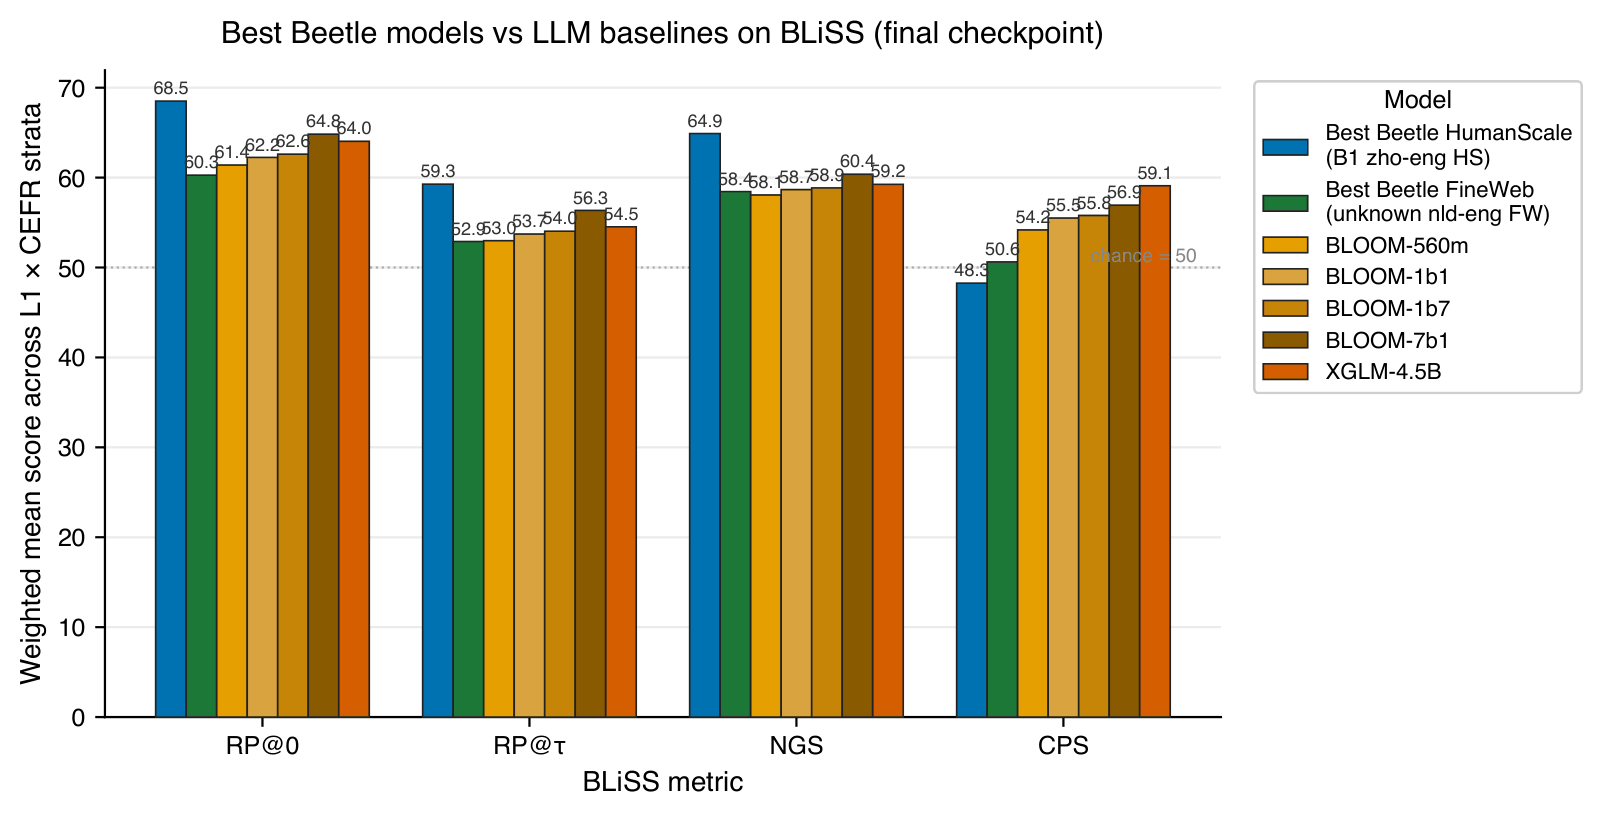
\includegraphics[width=1\linewidth]{fig/fig_best_bliss_vs_baselines-1.png}
    \caption{Best Beetle HumanScale (B1 zho-eng) — wins RP@0 at 68.5 and NGS at 64.9 Best Beetle FineWeb (B5 nld-eng). BLOOM-560m / 1b1 / 1b7 / 7b1. XGLM-4.5B — wins CPS at 59.1
}
    \label{fig:placeholder}
\end{figure}



\begin{figure}[!ht]
    \centering
    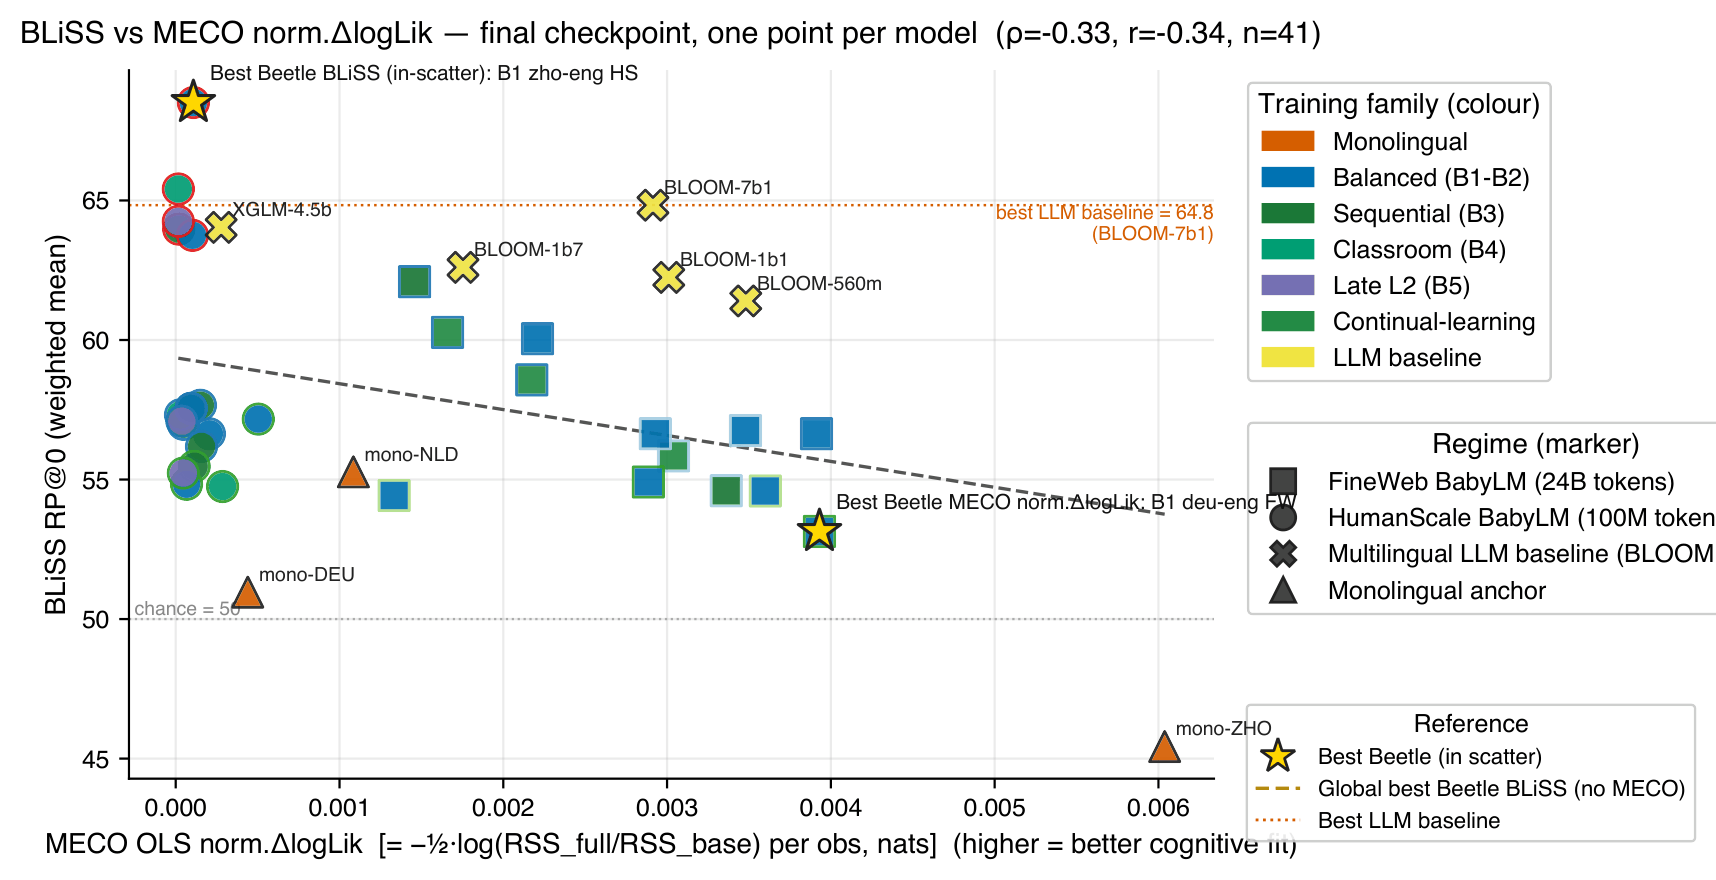
\includegraphics[width=1\linewidth]{fig/fig_bliss_vs_meco_final-1.png}
    \caption{Enter Caption}
    \label{fig:placeholder}
\end{figure}


\subsection{Eye Tracking During Reading}

\autoref{fig:meco} reports normalized log-likelihood improvements over baseline, enabling direct comparison across \raisebox{-0.3em}{\includegraphics[height=1.2em]{fig/BeetleLM.png}} and LLMs models grouped by L1 and training regime. Across all three languages, surprisal significantly improves model fit over the baselines. For Dutch (\texttt{nld}), standard multilingual models such as XGLM, EuroLLM, Aya, and Apertus yield relatively modest gains (≈6–39 in normalized log-likelihood), whereas all \raisebox{-0.3em}{\includegraphics[height=1.2em]{fig/BeetleLM.png}} variants show substantially larger improvements. In particular, the bilingual balanced model achieves the strongest performance (+110.67), followed by the simultaneous (+88.43) and monolingual (+84.26) variants. This suggests that, for Dutch, incorporating bilingual exposure—especially in a balanced regime—yields surprisal estimates that better align with human reading behavior than both monolingual training and large-scale multilingual baselines. For Chinese (\texttt{zho}) and German (\texttt{deu}), the advantage of \raisebox{-0.3em}{\includegraphics[height=1.2em]{fig/BeetleLM.png}} models becomes even more pronounced, though with different optimal training regimes. In Chinese, the simultaneous bilingual model performs best (+140.40), outperforming both the balanced (+112.32) and monolingual (+94.82) variants, as well as all baseline models. In German, we observe the largest overall gains, with the simultaneous \raisebox{-0.3em}{\includegraphics[height=1.2em]{fig/BeetleLM.png}} achieving a striking +300.67 improvement, followed by the monolingual (+240.55) and balanced (+197.86) variants. Notably, while strong baselines such as Aya and EuroLLM perform competitively in German (up to +182.25 and +105.60, respectively), they still fall well short of the best \raisebox{-0.3em}{\includegraphics[height=1.2em]{fig/BeetleLM.png}} configurations.



% \subsection{Psychometric Fit}

\begin{figure}[!ht]
    \centering
    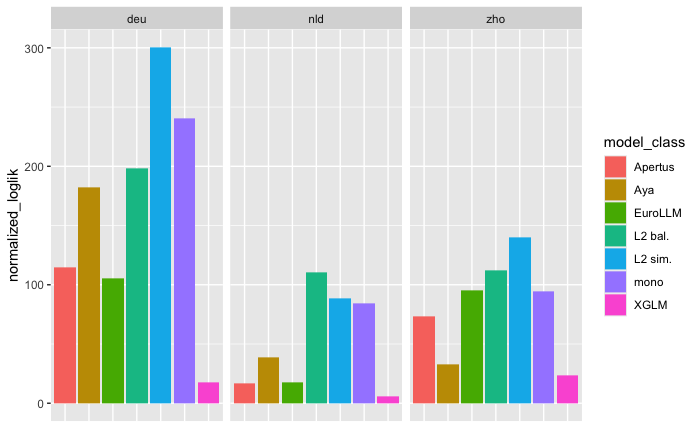
\includegraphics[width=\linewidth]{fig/meco_results_draft.png}
    \caption{MECO  \citep{siegelman2025wave} Alignment Results for \raisebox{-0.3em}{\includegraphics[height=1.2em]{fig/BeetleLM.png}}  monolingual \texttt{nld, zho,deu} and bilingual models (L1 \texttt{nld, deu, zho} and L2 \texttt{eng}) with \texttt{balanced/simultaneous} exposure curricula . Detailed results can be found in \autoref{tab:loglik} \catherine{Todo: re-plot in the same style/color-coding as the other plots. or maybe this is better as a table?} }
    \label{fig:meco}
\end{figure}

\subsection{Age-of-Acquisition Norms}

\suchir{We can ask whether our bilingual models better model AoA norms etc. compared to monolingual models.}

\subsection{Effect of Learning Rate}
\suchir{We investigate the effect of learning rate on MECO for simultaneous bilingual conditions. }

%\begin{itemize}
%    \item 1-2 language pairs
%    \item only RT task (one task)
%    \item 1 bilingual condition, e.g. simultaneous
%\end{itemize}

\section{Discussion}



\paragraph{Other Bilingual Conditions.}
What would it look like to model, e.g. heritage?

\section{Conclusion}

% We presented a framework, \raisebox{-0.3em}{\includegraphics[height=1.2em]{fig/BeetleLM.png}},  that recasts polyglot language model pretraining as a controlled dynamical system, enabling causal investigation of how exposure timing and control parameters related to catastrophic forgetting shape cross-lingual multilingual acquisition during pretraining. Downstream results show data input quantity and ordering has a measurable impact on downstrem performance Human-scale language modelling experiments reveal near-balanced exposure schedules achieve higher alignment to multilingual reading behaviour than state-of-the-art multilingual LLMs, highlighting empirical benefits of \raisebox{-0.3em}{\includegraphics[height=1.2em]{fig/BeetleLM.png}}'s conceptual decoupling of \textit{acquisition timing} from \textit{data quantity}; the introduction of parameterised exposure schedules, and integration both stability-oriented and adaptation-oriented control mechanisms.




%within pretraining has the potential to become a valuable framework for developing computational models of natural language learning for developing cognitive proxies. It directly addresses a common criticism leveraged by cognitive scientists to Dynamical Systems approaches to multilingual language learning– which to our knowledge has had no computational implementation \citep{lenzing2022lost, ionin2007dst, pienemann2024can, pallotti2022cratylus}. 

%But studying bilingualism is often limited by inter-speaker differences and limited population size (with a particular language experience) (basically it's easier to find Spanish-English bilinguals than English-Spanish bilinguals)


%\subsection{Cross-lingual Alignment Dynamics}

%sequential curricula produce delayed alignment in mid-layers, while simultaneous exposure induces early shared manifolds.


%\subsection{Forward Transfer and Interference}
%Sequential L2 exposure induces measurable backward interference, mitigated when using part-time exposure schedules. Gradient geometry confirms these patterns.

%\subsection{Neuron and Circuit Analysis}
%Shared neurons and OV circuits form early in simultaneous regimes; sequential curricula create more language-specific circuits. Attention heads show selective mapping between languages, consistent with bilingual cognitive theories.

%\section{Conclusion}

\section{Limitations}

\paragraph{Limited Scale} Due to the limited compute resources, we only included models of up to 350M parameters in size for training, and multilingual LMs 70B parameters for baseline comparison. Modern LMs are orders of magnitude larger in parameter count, and it is important to test if the trends identified would hold for larger sizes. 

\paragraph{Eye-Tracking} \suchir{This work, consistent with most computational studies of surprisal only focus on gaze duration (Aurnhammer \& Frank 2019; Smith \& Levy 2013); we don't really consider other cognitively-relevant eye-tracking metrics.}  

\paragraph{Limited Selection of Bilingual and L2 Psycho- and Neuro-Linguistic Studies} The reported results in the paper only focus on established eye-tracking second-language learning datasets. However, there is a rich literature of bilingual neurolinguistic datasets which can be used to analyse the Beetle models. We leave careful treatment and investigation of neurolinguistic alignment to further work.  We hope to replicate monolingual English findings on correlations of brain signals (e.g., N400/P600) to LM surprisals  \citep{michaelov2026better}. 


\paragraph{Effect of Data Quality} Although reported experiments conduct minimal evaluation decontamination in \texttt{beetle-data}, there exist other training techniques, such as Filtered Corpus Training \citep{patil2024filtered}, which can provide more robust generalisation bounds.  

\paragraph{Psycholinguistic and Pedagogical Evaluation on L2 English} This is an issue for BLiSS, but we can use MultilingualCEFR. Limited L2 eye-tracking data beyond English L2. 

\paragraph{Bilingual Acquisition beyond Language Model Pretraining} \suchir{ Some things which we probably can't take account of: Input amount is only one aspect of the bilingual experience (e.g., input \textit{quality} is a discussed) \citep{luk2013bilingualism, carroll2017exposure, de2017role, paradis2023sources}; social interaction and pragmatics are not simulated.}




\section{Notes}

\suchir{\textbf{A note on the title:} Catherine suggested “Training Plausible Bilingual Models” as a possible title – but I marginally prefer \textit{human-like} over \textit{plausible} (makes more sense to general NLP audience?). Also I think we can say \textit{multilingual} in the title, since Beetle supports this. I think we can report non-MECO/psycholinguistic evals for trilingual in this paper.}


%\raisebox{-0.3em}{\includegraphics[height=1.2em]{fig/\raisebox{-0.3em}{\includegraphics[height=1.2em]{fig/BeetleLM.png}}.png}}

\suchir{the paper's main contributions are 1) expanding on the B-GPT models and creating a flexible training framework for making more models in more bilingual conditions to model a wider range of language experience types 2) comparing human-scale data and fineweb data 3) validating "plausible" training regimes with reading time. comparing with EWC is probably more important, since the main contribution of the paper is a training framework. And so we should compare with the other method – MAML?}


%Beetle combines input structure (data/exposure curricula), plasticity through learning rate schedules and MAML, and memory ( i.e. forgetting) constraints. 

\url{https://arxiv.org/pdf/2604.07067}
\url{https://arxiv.org/pdf/2603.29552}






\subsection{Old Intro}
\suchir{From Catherine – crosslingual transfer, how to create more balanced performance, influence of design decisions}

The majority of state-of-the-art language models are (massively) multilingual, but there are still many aspects of multilinguality that are not understood. Studying multilinguality in a bilingual setting allows for more controlled experimentation to develop a better understanding of how a language model represents two different languages \cite{inaba-etal-2025-bilingual}.  

At the same time, as language models become more performant, they are increasingly being used to model aspects of human language processing and production \catherine{add citations}, particularly through human-scale pretraining \cite{warstadt2023findings, warstadt2024insights, hu2024findings, charpentier2025findings,  wilcox2025bigger, choshen2026babylm}.  As the vast majority of the world is multilingual  \cite{garcia2012cognitive, de2015multilingual, tucker1998global}, it is impossible to fully understand human language acquisition and processing without understanding bilingual and multilingual language processing. 

%acquiring different languages to differing proficiencies across a lifetimes.

In this work, we introduce a \raisebox{-0.3em}{\includegraphics[height=1.2em]{fig/BeetleLM.png}}, a framework for training controlled, developmentally plausible bilingual language models. %a \textit{longitudinal interpretability framework for bilingual language models}.  
Building on previous work, which either relies on static \catherine{homogenous? i feel like we want to say the same throughout training - not sure how much static conveys this.} data mixtures or uses relatively coarse cognitively-inspired curriculum learning \cite{oba-etal-2023-second, aoyama2024modeling, arnett-etal-2025-acquisition}, our framework formalises multilingual acquisition as a time-dependent dynamical system by training autoregressive language models with explicitly controlled exposure schedules that vary the relative contribution of each language over the course of training. Our framework enables several classes of analyses that are currently underexplored. 

In the current paper, we pretrain a variety of bilingual models to test the effects of both human-scale versus compute-optimal dataset size and also the order and duration of L1 and L2 exposure. We also demonstrate that our framework can be extended to other multilingual settings, e.g. trilingual exposure. We compare our data-driven training method with existing methods of training bilingual mechanisms, namely Elastic Weight Consolidation \catherine{citation; summary of comparison}. 
% First, we pretrain human-scale bilingual and trilingual language models with fixed token budgets while varying the order and duration of language exposure during pretraining. Second, we compare different data mixtures within different phases of bilingual and trilingual human-scale language model pretraining to approximate a wider range of naturalistic language learning settings.  Finally, we further introduce a separation between external data-driven learning dynamics and internal control mechanisms, incorporating both Elastic Weight Consolidation and meta-learning within pretraining as complementary interventions on the stability–plasticity tradeoff.   
Together, \raisebox{-0.3em}{\includegraphics[height=1.2em]{fig/BeetleLM.png}} supports a new class of analyses over training trajectories, including representational alignment, cross-lingual transfer, and catastrophic forgetting, providing a controlled and reproducible setting for studying the dynamics of polyglot language acquisition.


%First, we investigate the temporal dynamics of cross-lingual representational alignment across layers and training stages. Second, we analyse transfer and interference between languages using gradient geometry and parameter reuse metrics. Third, we study circuit-level mechanisms underlying multilingual integration by tracking the evolution of attention and feedforward substructures. Fourth, we examine token-level lexical learning trajectories, enabling direct analysis of cross-lingual transfer at the level of individual lexical items. Finally, we investigate forgetting and representational drift induced by second-language exposure. Studying the causal dynamics of memorization, tokenization, and transfer in multilingual or bilingual language models requires several key considerations: (i) models with fully accessible checkpoints, (ii) transparent pre-training data, and (iii) controlled language coverage to enable interpretable cross-lingual analysis.

% By combining controlled acquisition schedules with full training traceability, our framework provides a novel empirical platform for studying bilingual representation emergence in neural language models. More broadly, this work contributes toward a mechanistic understanding of multilingual learning and provides a bridge between interpretability research, continual learning theory, and computational models of bilingual cognition.

 \section{Acknowledgements}
This work is supported by Cambridge University Press \& Assessment. Compute facilities were provided by EleutherAI. The authors would like to wholeheartedly thank the helpful and insightful comments from members of the Cambridge NLIP group (in alphabetical order, surname): Laura Barbenel, Andrew Caines, Bianca Ganescu, Lily Goulder, Denise Lofflad, Aoife O'Driscoll. The manuscript has been greatly improved in no small part due to their efforts. The authors would also like to thank Tatsuya Aoyama (and Tyler Chang?) for advice about data streaming and the CELER evaluation datasets. 

% Entries for the entire Anthology, followed by custom entries
\bibliography{anthology,custom}
\bibliographystyle{acl_natbib}

\newpage
\appendix
\onecolumn

\section*{Appendix}
\noindent\rule{\linewidth}{0.4pt}

\begin{tabular}{ll}
A.1 & \hyperref[sec:lit-review]{Comparison of Beetle and L2LMs} \\
A.2 & \hyperref[sec:train]{\raisebox{-0.3em}{\includegraphics[height=1.2em]{fig/BeetleLM.png}} Training Framework} \\
A.3 & \hyperref[sec:beetle-curricula]{\raisebox{-0.3em}{\includegraphics[height=1.2em]{fig/BeetleLM.png}} Curricula} \\
A.4 & \hyperref[sec:beetle-control-parameters]{\raisebox{-0.3em}{\includegraphics[height=1.2em]{fig/BeetleLM.png}} Control Parameters} \\
A.5 & \hyperref[sec:beetle-data]{Beetle-Data} \\
A.6 & \hyperref[sec:sec:beetle-experiments]{Reported Experimental Conditions} \\
A.7 & \hyperref[sec:beetle-analyze]{Beetle Analyze} \\
A.8 & \hyperref[sec:aoa-results]{Detailed AoA Results} \\
A.9 & \hyperref[sec:meco-results]{Detailed MECO Results} \\
A.10 & \hyperref[sec:meco-results]{Detailed Downstream Results} \\

\end{tabular}

\noindent\rule{\linewidth}{0.4pt}




\newpage 



\begin{table*}[t]
  \centering
  \small
  \caption{Model log-likelihood results by L2 language on the MECO wave-1 + wave-2 joined data (canonical pipeline, matching \texttt{stats/meco\_l2.Rmd}). For each model and L2 language we report $\log L$ of the full model, $\log L$ of the baseline (surprisal terms dropped), and $\Delta\log L = \log L(\text{full}) - \log L(\text{baseline})$; larger $\Delta\log L$ indicates better surprisal alignment with human reading times. Only models with a plottable MECO row are included.}
  \label{tab:meco_langrows}
  \begin{tabular}{lrrrl}
    \toprule
    Model & $\log L$ & Baseline $\log L$ & $\Delta\log L$ & Class \\
    \midrule
    \multicolumn{5}{l}{\textit{Dutch (\texttt{nld})}} \\
    \midrule
    XGLM-4.5b & $-194066.67$ & $-194075.32$ & $8.65$ & XGLM \\
    BLOOM-1b1 & $-194033.84$ & $-194075.32$ & $41.47$ & BLOOM \\
    BLOOM-1b7 & $-194040.91$ & $-194075.32$ & $34.41$ & BLOOM \\
    BLOOM-560m & $-194031.03$ & $-194075.32$ & $44.29$ & BLOOM \\
    BLOOM-7b1 & $-194055.62$ & $-194075.32$ & $19.69$ & BLOOM \\
    mono-nld & $-193979.29$ & $-194075.32$ & $96.02$ & mono-NLD \\
    mono-eng & $-194010.19$ & $-194075.32$ & $65.13$ & mono-ENG \\
    B1 eng-nld FW (FW) & $-194035.16$ & $-194075.32$ & $40.16$ & L2 bal. \\
    B1 nld-eng FW (FW) & $-194028.69$ & $-194075.32$ & $46.62$ & L2 bal. \\
    B1 nld-eng HS (HS) & $-194012.99$ & $-194075.32$ & $62.33$ & L2 bal. \\
    episodic nld-eng HS (HS) & $-194021.76$ & $-194075.32$ & $53.55$ & L2 bal. \\
    unknown eng-nld FW (FW) & $-194031.85$ & $-194075.32$ & $43.46$ & L2 bal. \\
    unknown nld-eng FW (FW) & $-194020.75$ & $-194075.32$ & $54.57$ & L2 bal. \\
    B2 eng-nld FW (FW) & $-194034.54$ & $-194075.32$ & $40.78$ & L2 sim. \\
    B2 nld-eng FW (FW) & $-193979.34$ & $-194075.32$ & $95.97$ & L2 sim. \\
    B2 nld-eng HS (HS) & $-193940.18$ & $-194075.32$ & $135.14$ & L2 sim. \\
    ewc nld-eng HS (HS) & $-193940.18$ & $-194075.32$ & $135.14$ & L2 sim. \\
    lamol nld-eng HS (HS) & $-193940.18$ & $-194075.32$ & $135.14$ & L2 sim. \\
    B3-0 nld-eng HS (HS) & $-193936.56$ & $-194075.32$ & $138.75$ & L2 seq. \\
    B3-33 eng-nld FW (FW) & $-194035.66$ & $-194075.32$ & $39.66$ & L2 seq. \\
    B3-33 nld-eng FW (FW) & $-193999.94$ & $-194075.32$ & $75.37$ & L2 seq. \\
    B3-33 nld-eng HS (HS) & $-193935.73$ & $-194075.32$ & $139.58$ & L2 seq. \\
    B4 nld-eng HS (HS) & $-193953.55$ & $-194075.32$ & $121.77$ & L2 class. \\
    B5 nld-eng HS (HS) & $-193937.57$ & $-194075.32$ & $137.74$ & L2 late \\
    \midrule
    \multicolumn{5}{l}{\textit{Chinese (\texttt{zho})}} \\
    \midrule
    XGLM-4.5b & $-234098.92$ & $-234121.53$ & $22.60$ & XGLM \\
    BLOOM-1b1 & $-233957.22$ & $-234121.53$ & $164.30$ & BLOOM \\
    BLOOM-1b7 & $-233984.47$ & $-234121.53$ & $137.06$ & BLOOM \\
    BLOOM-560m & $-233972.28$ & $-234121.53$ & $149.25$ & BLOOM \\
    BLOOM-7b1 & $-234036.80$ & $-234121.53$ & $84.73$ & BLOOM \\
    mono-zho & $-234116.14$ & $-234121.53$ & $5.39$ & mono-ZHO \\
    mono-eng & $-234070.70$ & $-234121.53$ & $50.83$ & mono-ENG \\
    B1 zho-eng HS (HS) & $-234015.83$ & $-234121.53$ & $105.69$ & L2 bal. \\
    B2 zho-eng HS (HS) & $-234021.38$ & $-234121.53$ & $100.14$ & L2 sim. \\
    B3-33 zho-eng HS (HS) & $-234018.37$ & $-234121.53$ & $103.15$ & L2 seq. \\
    B4 zho-eng HS (HS) & $-234022.81$ & $-234121.53$ & $98.71$ & L2 class. \\
    B5 zho-eng HS (HS) & $-234006.13$ & $-234121.53$ & $115.40$ & L2 late \\
    \midrule
    \multicolumn{5}{l}{\textit{German (\texttt{deu})}} \\
    \midrule
    XGLM-4.5b & $-275354.57$ & $-275373.57$ & $19.00$ & XGLM \\
    BLOOM-1b1 & $-275193.91$ & $-275373.57$ & $179.66$ & BLOOM \\
    BLOOM-1b7 & $-275222.85$ & $-275373.57$ & $150.71$ & BLOOM \\
    BLOOM-560m & $-275191.60$ & $-275373.57$ & $181.96$ & BLOOM \\
    BLOOM-7b1 & $-275257.67$ & $-275373.57$ & $115.90$ & BLOOM \\
    mono-deu & $-275239.27$ & $-275373.57$ & $134.29$ & mono-DEU \\
    mono-eng & $-275303.30$ & $-275373.57$ & $70.26$ & mono-ENG \\
    B1 deu-eng FW (FW) & $-275248.33$ & $-275373.57$ & $125.24$ & L2 bal. \\
    B1 deu-eng HS (HS) & $-275298.46$ & $-275373.57$ & $75.10$ & L2 bal. \\
    B1 eng-deu FW (FW) & $-275209.05$ & $-275373.57$ & $164.52$ & L2 bal. \\
    B2 deu-eng FW (FW) & $-275188.90$ & $-275373.57$ & $184.66$ & L2 sim. \\
    B2 deu-eng HS (HS) & $-275207.30$ & $-275373.57$ & $166.27$ & L2 sim. \\
    B2 eng-deu FW (FW) & $-275295.18$ & $-275373.57$ & $78.39$ & L2 sim. \\
    B3-33 deu-eng HS (HS) & $-275196.11$ & $-275373.57$ & $177.45$ & L2 seq. \\
    B4 deu-eng HS (HS) & $-275233.00$ & $-275373.57$ & $140.57$ & L2 class. \\
    B5 deu-eng HS (HS) & $-275205.21$ & $-275373.57$ & $168.36$ & L2 late \\
    \bottomrule
  \end{tabular}
\end{table*}




% Table 6: Canonical MECO ΔlogLik (matches stats/meco_l2.Rmd)
% Requires \usepackage{booktabs} in preamble
\begin{table*}[t]
  \centering
  \small
  \caption{Canonical MECO reading-time alignment, matching the R \texttt{lmer} pipeline in \texttt{stats/meco\_l2.Rmd}. For each (model, L2 language) we fit
\begin{center}\footnotesize
\texttt{firstrun.dur \textasciitilde{} scale(Surprisal) + scale(Surprisal1p) + scale(Surprisal2p) + scale(wordnum) + scale(wlen\{,1p,2p\}) + scale(freq\{,1p,2p\}) + (1 + \textlangle same\textrangle{} \textbardbl{} subid), REML=FALSE}
\end{center}
and report $\Delta\log L = \log L(\text{full}) - \log L(\text{baseline})$, where the baseline drops the three Surprisal terms. Boundary words per (itemid, sentnum) are excluded; word frequency is Zipf~\texttt{wordfreq} computed against the English corpus for all L2 subsets. Fit backend: statsmodels|re=1+vc(||).}
  \label{tab:meco}
  \begin{tabular}{lrrrrrrrrr}
    \toprule
    \multicolumn{10}{l}{\textit{Panel A — Group means per canonical L2 language}} \\
    \midrule
    Group & $N_{\text{Dutch}} $ & $\overline{\Delta\log L}_{\text{Dutch}} $ & $\bar{\beta}_{\text{Dutch}} $ & $N_{\text{German}} $ & $\overline{\Delta\log L}_{\text{German}} $ & $\bar{\beta}_{\text{German}} $ & $N_{\text{Chinese}} $ & $\overline{\Delta\log L}_{\text{Chinese}} $ & $\bar{\beta}_{\text{Chinese}} $ \\
    \midrule
    Beetle bilingual & 33 & \textbf{81.10} & 12.65 & 33 & \textbf{167.04} & 15.98 & 33 & 130.41 & 18.12 \\
    Bilingual LLM & 1 & 8.65 & 3.51 & 1 & 19.00 & 4.36 & 1 & 22.60 & 5.33 \\
    BLOOM (ladder) & 4 & 34.96 & 7.85 & 4 & 157.06 & 13.39 & 4 & \textbf{133.83} & 14.08 \\
    Monolingual anchors & 4 & 56.85 & 12.40 & 4 & 105.81 & 13.96 & 4 & 40.22 & 10.06 \\
    \midrule
    \multicolumn{10}{l}{\textit{Panel B — Per-model extremes (mean over L2 languages)}} \\
    \midrule
    Model & $k$ & $\overline{\Delta\log L}$ & $\bar{\beta}_{\text{Surprisal}}$ \\
    \midrule
    \textit{Top 5 by $\Delta\log L$} \\
    B3-33 nld-eng HS & 3 & 170.03 & 17.99 \\
    B5 nld-eng HS & 3 & 168.44 & 17.93 \\
    lamol nld-eng HS & 3 & 166.79 & 17.80 \\
    B2 nld-eng HS & 3 & 166.79 & 17.80 \\
    ewc nld-eng HS & 3 & 166.79 & 17.80 \\
    \midrule
    \textit{Bottom 5 by $\Delta\log L$} \\
    mono-ZHO & 3 & 8.63 & 3.30 \\
    XGLM-4.5b & 3 & 16.75 & 4.40 \\
    B1 deu-eng HS & 3 & 53.46 & 10.35 \\
    mono-ENG & 3 & 62.07 & 12.19 \\
    B2 eng-deu FW & 3 & 64.02 & 11.76 \\
    \bottomrule
  \end{tabular}
\end{table*}


\newpage

\section{Figures}

\begin{figure}[!ht]
    \centering
    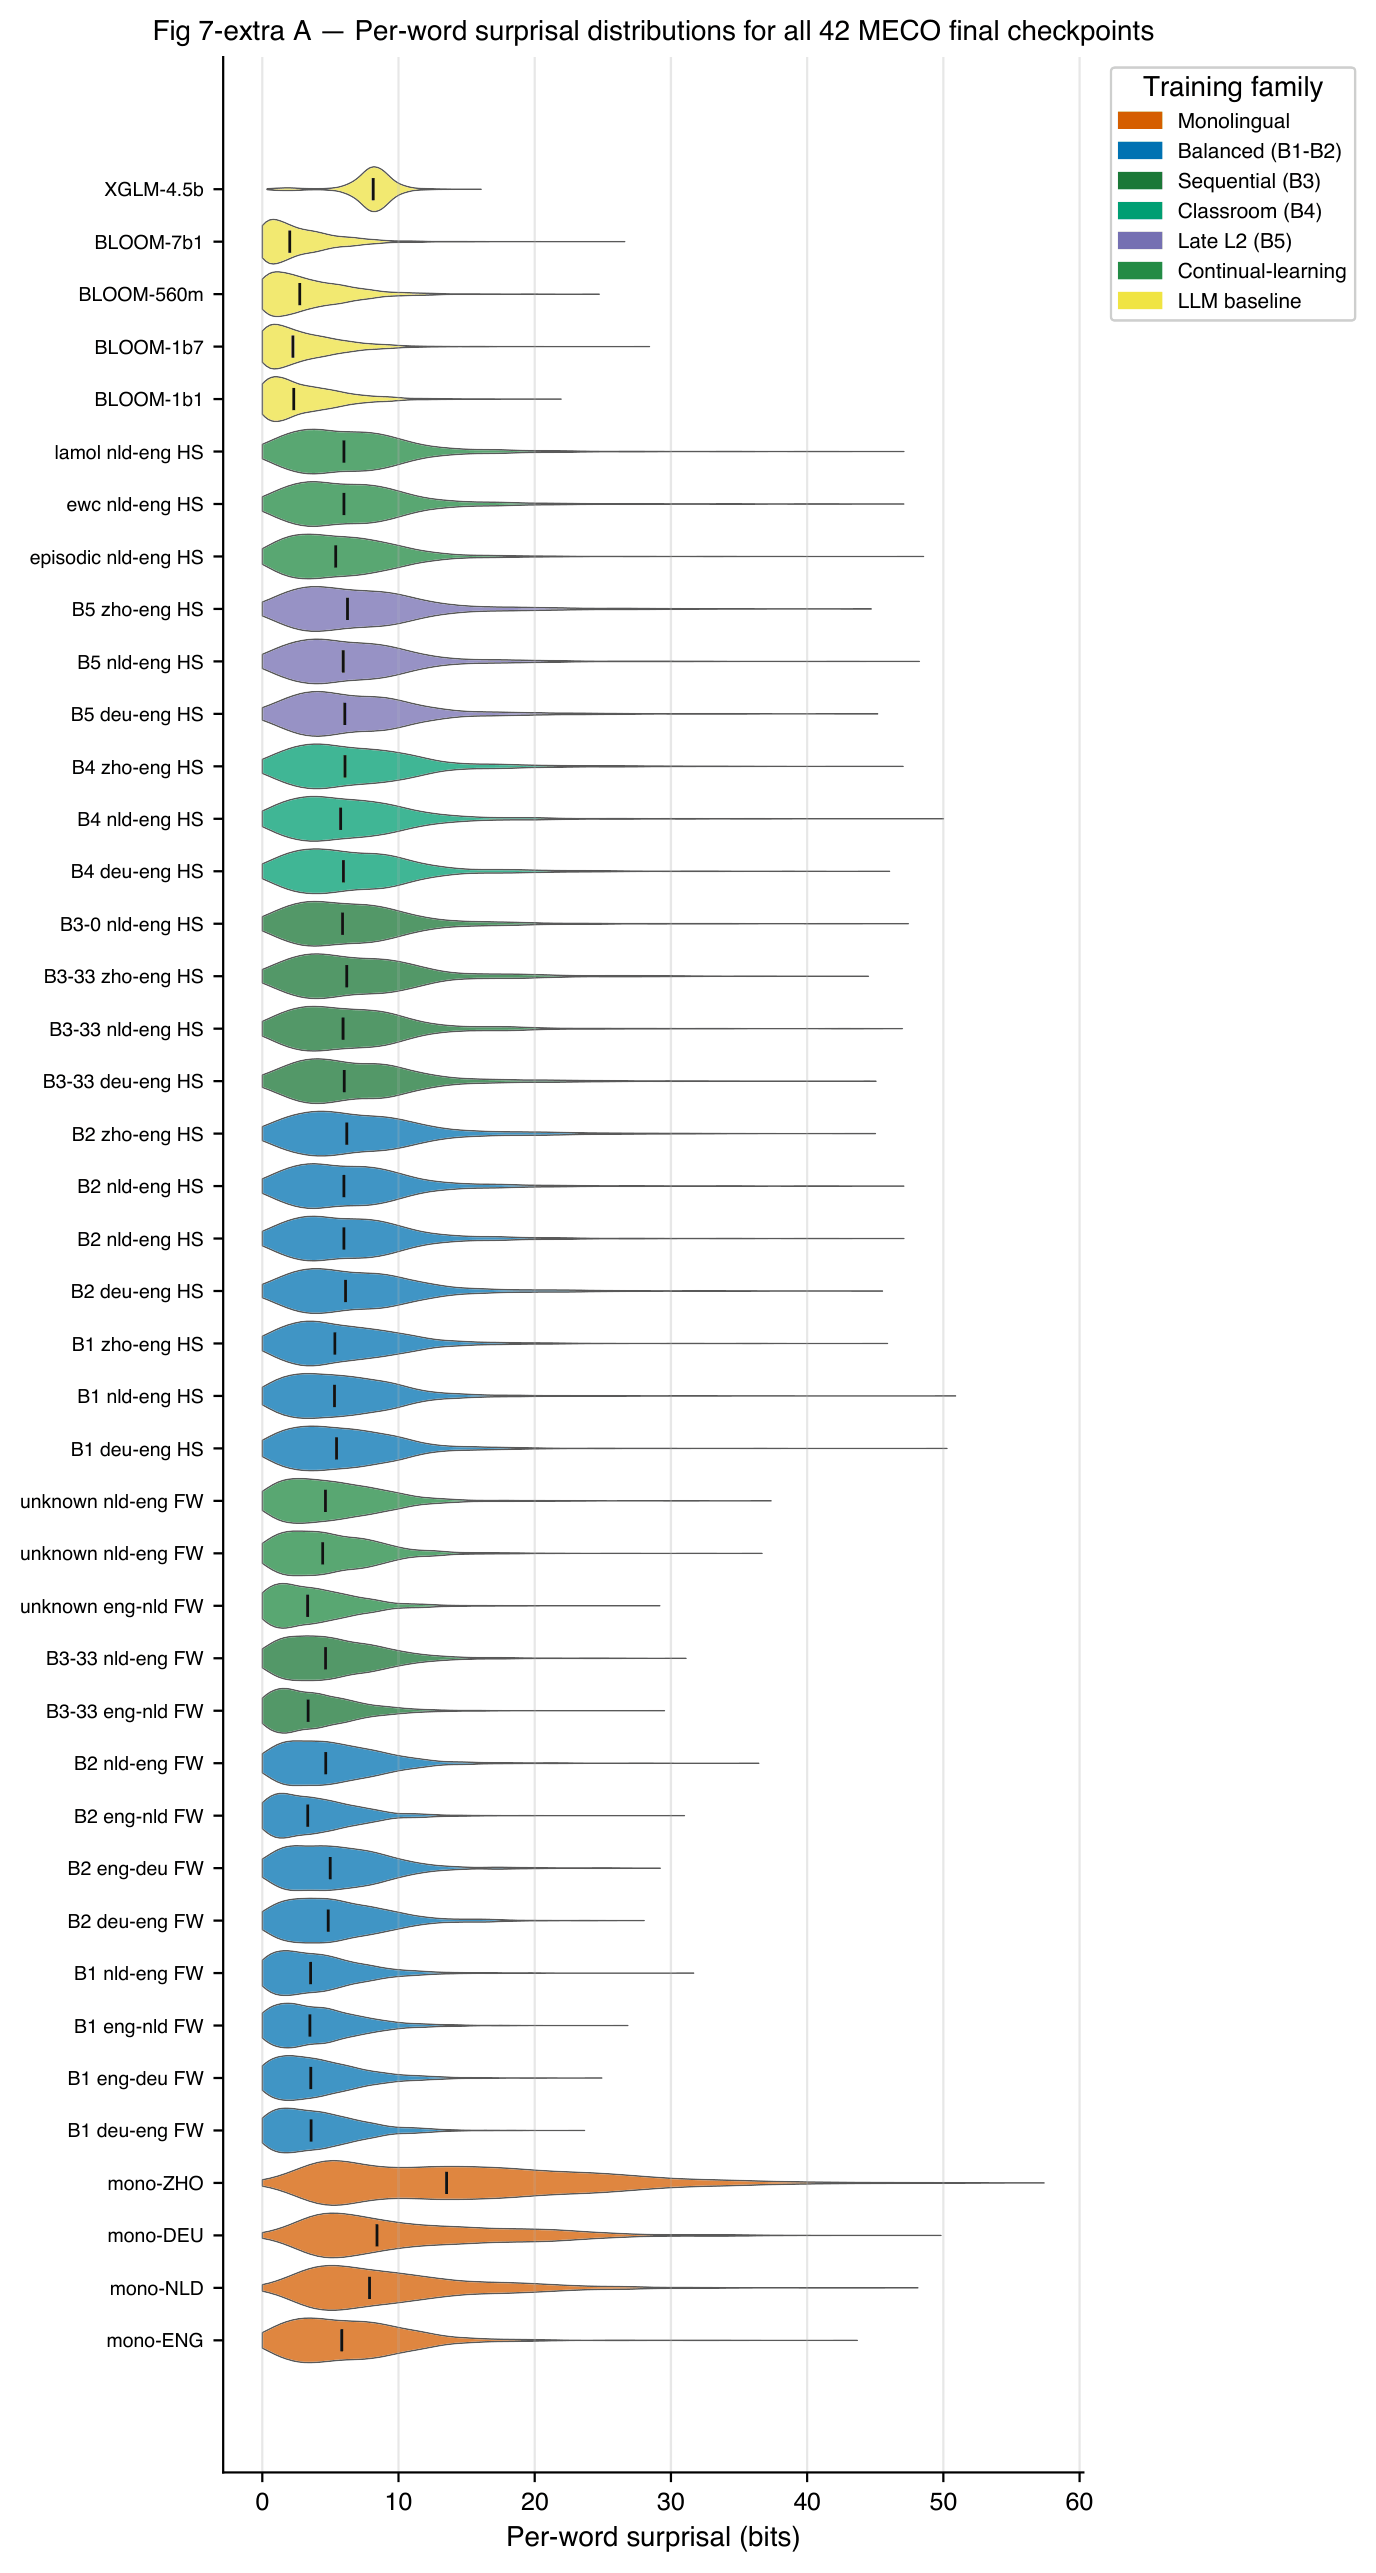
\includegraphics[width=0.5\linewidth]{fig/fig7_extra_a_all_final_violins-1.png}
    \caption{Enter Caption}
    \label{fig:placeholder}
\end{figure}
\newpage 

\begin{figure}[!ht]
    \centering
    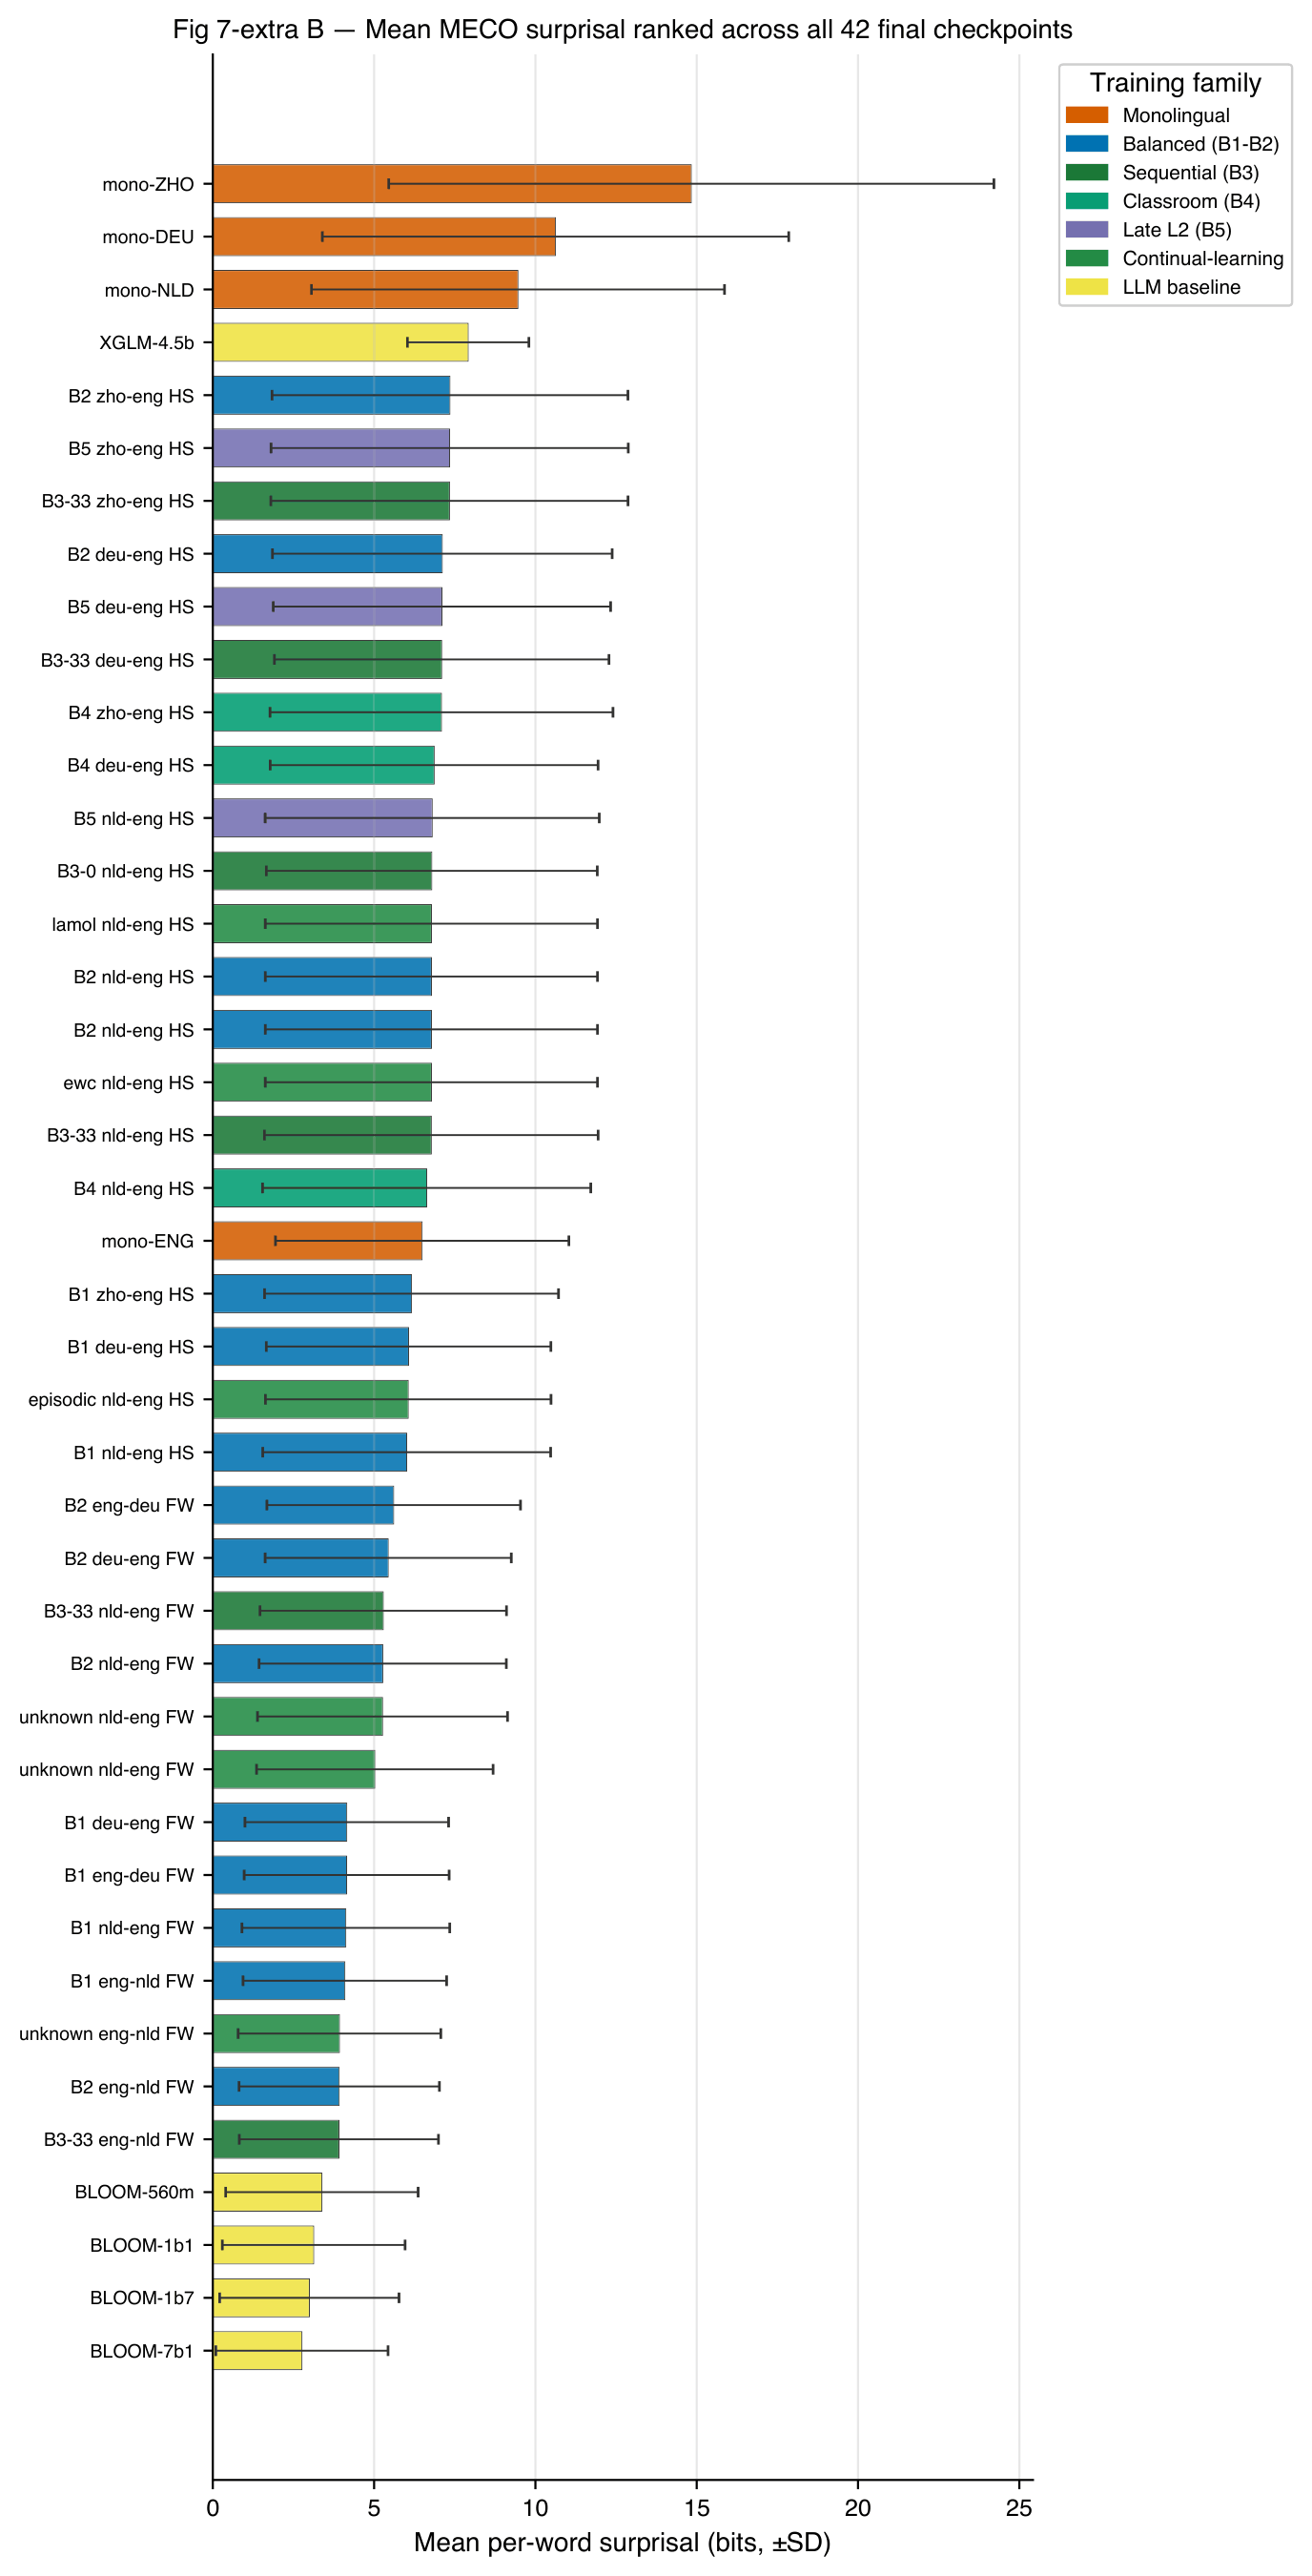
\includegraphics[width=0.5\linewidth]{fig/fig7_extra_b_all_final_ranked_bar-1.png}
    \caption{Enter Caption}
    \label{fig:placeholder}
\end{figure}



\newpage 

\begin{figure}
    \centering
    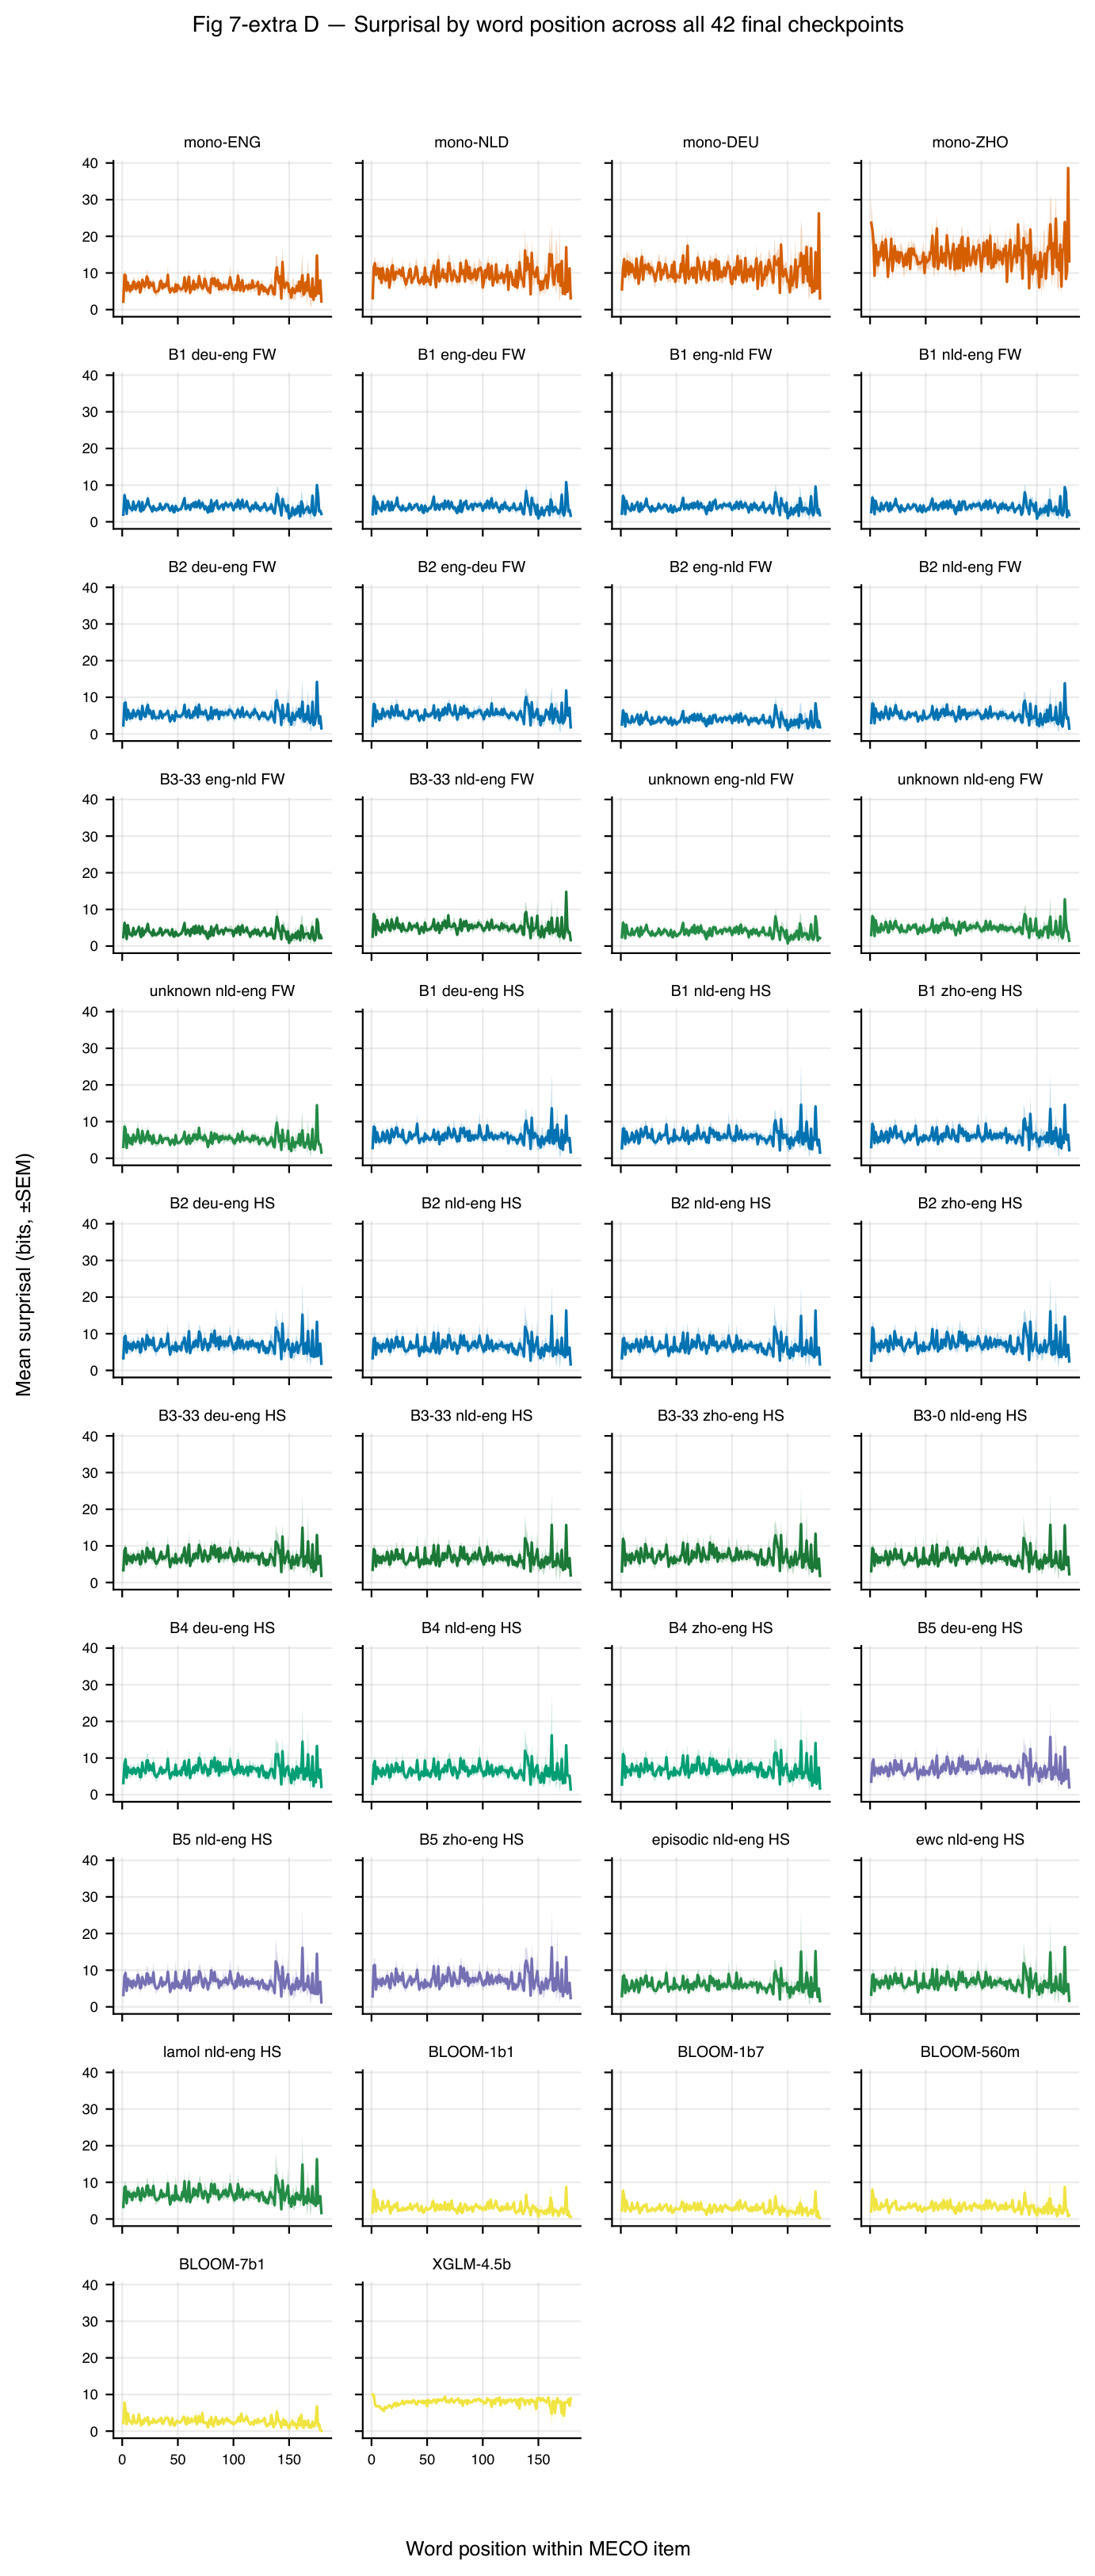
\includegraphics[width=0.5\linewidth]{fig/fig7_extra_d_all_final_wordnum_trace-1.png}
    \caption{Enter Caption}
    \label{fig:placeholder}
\end{figure}
\newpage 

\begin{figure}[!ht]
    \centering
    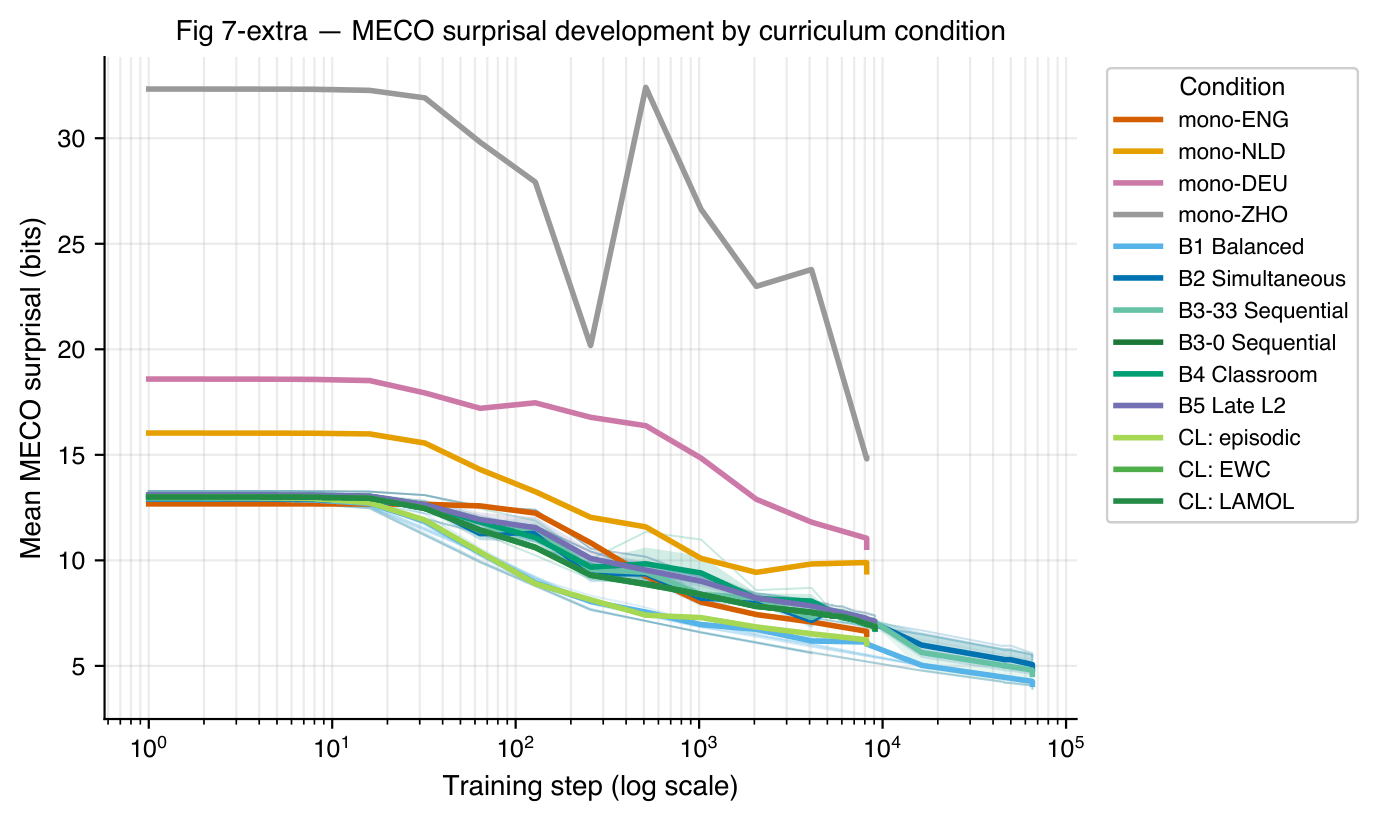
\includegraphics[width=0.5\linewidth]{fig/fig7_extra_dev_by_curriculum-1.png}
    \caption{Enter Caption}
    \label{fig:placeholder}
\end{figure}

\newpage 

\begin{figure}[!ht]
    \centering
    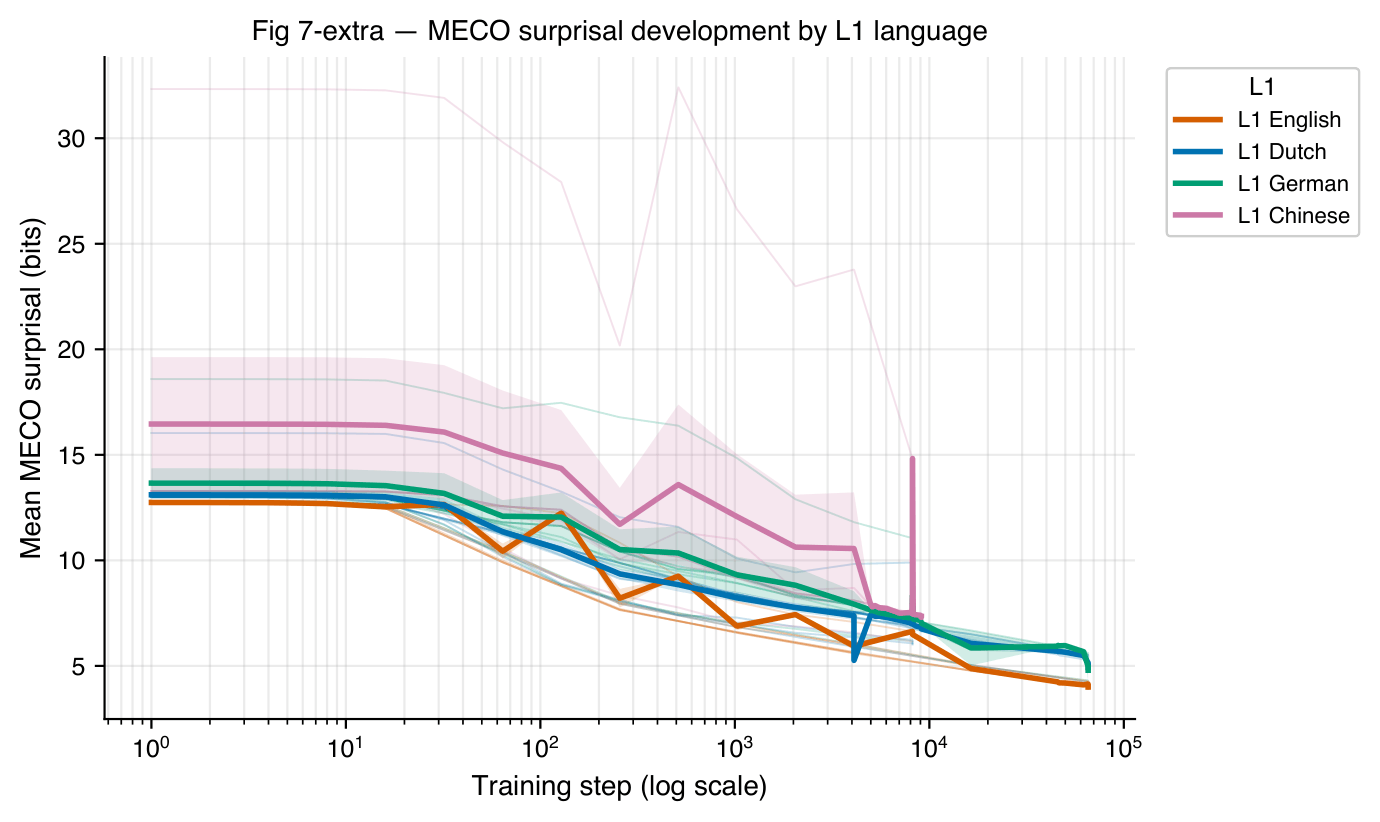
\includegraphics[width=0.5\linewidth]{fig/fig7_extra_dev_by_l1_language-1.png}
    \caption{Enter Caption}
    \label{fig:placeholder}
\end{figure}

\newpage 

\begin{figure}[!ht]
    \centering
    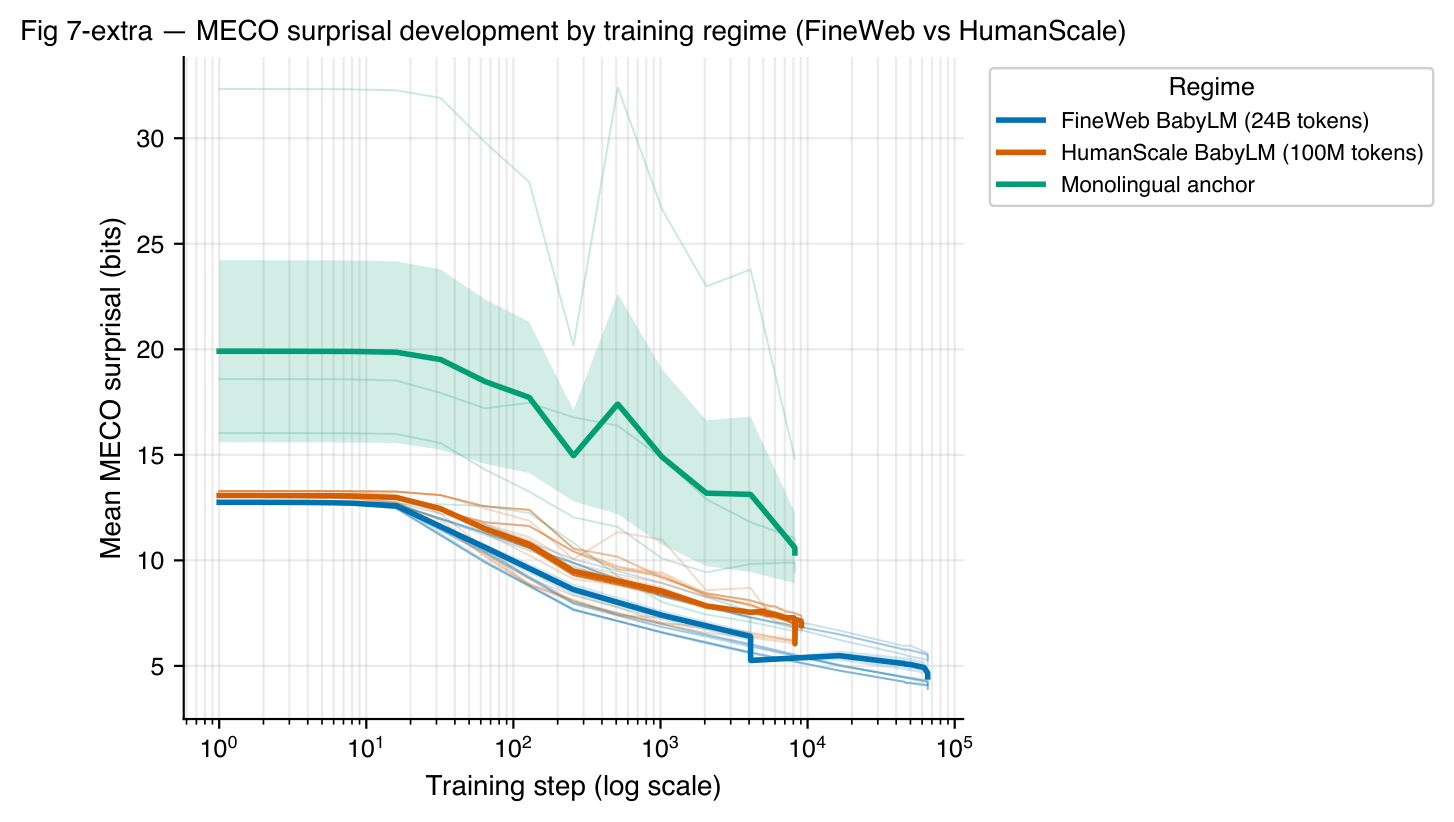
\includegraphics[width=0.5\linewidth]{fig/fig7_extra_dev_fineweb_vs_humanscale-1.png}
    \caption{Enter Caption}
    \label{fig:placeholder}
\end{figure}

\newpage 


\begin{figure}[!ht]
    \centering
    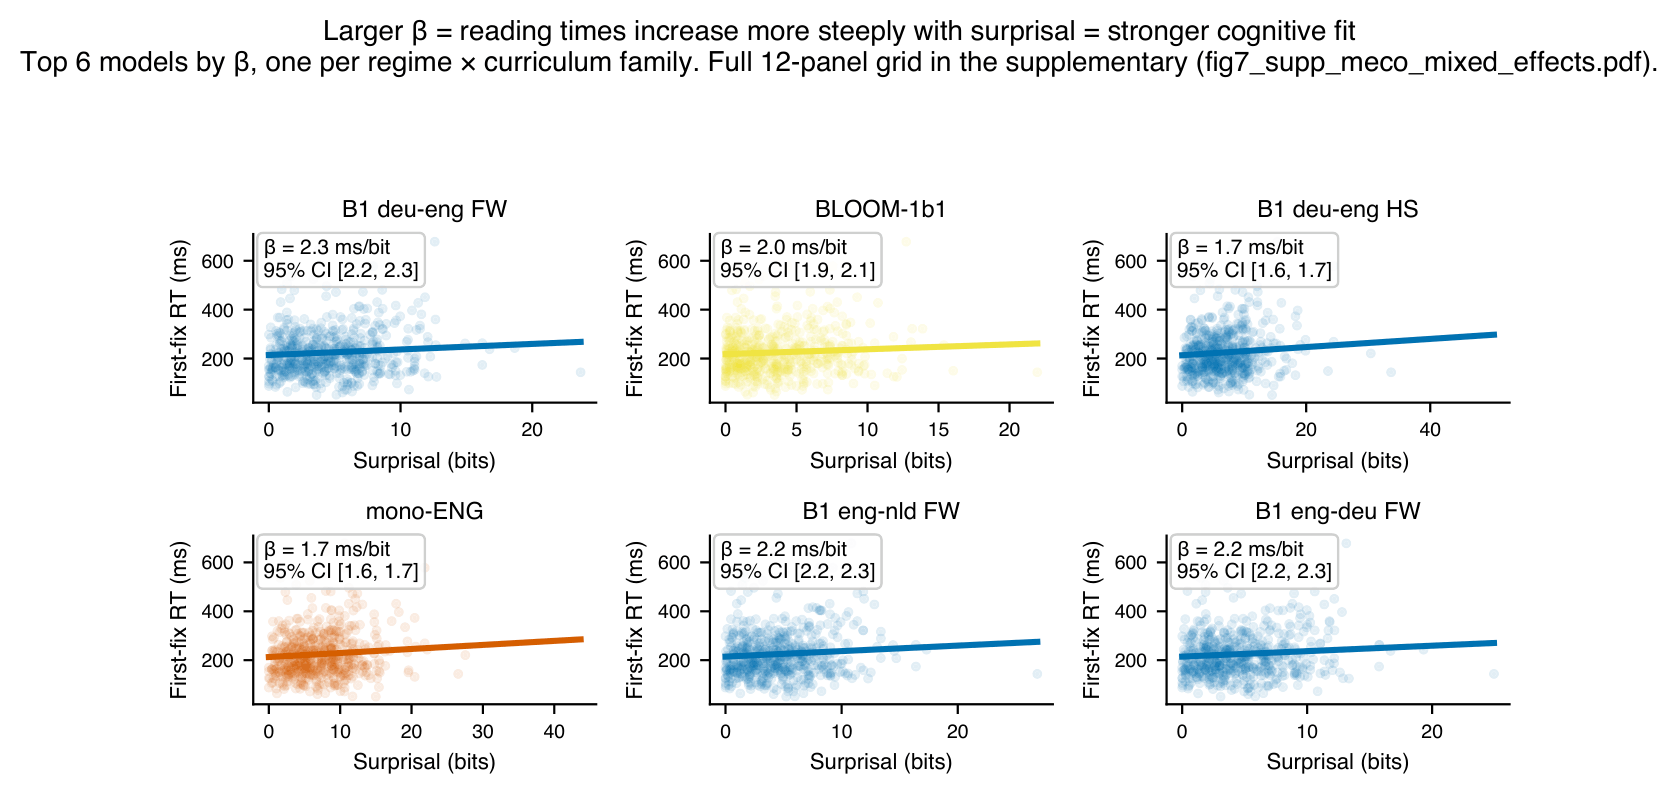
\includegraphics[width=0.5\linewidth]{fig/fig7_meco_mixed_effects-1.png}
    \caption{Enter Caption}
    \label{fig:placeholder}
\end{figure}
\newpage 

\begin{figure}[!ht]
    \centering
    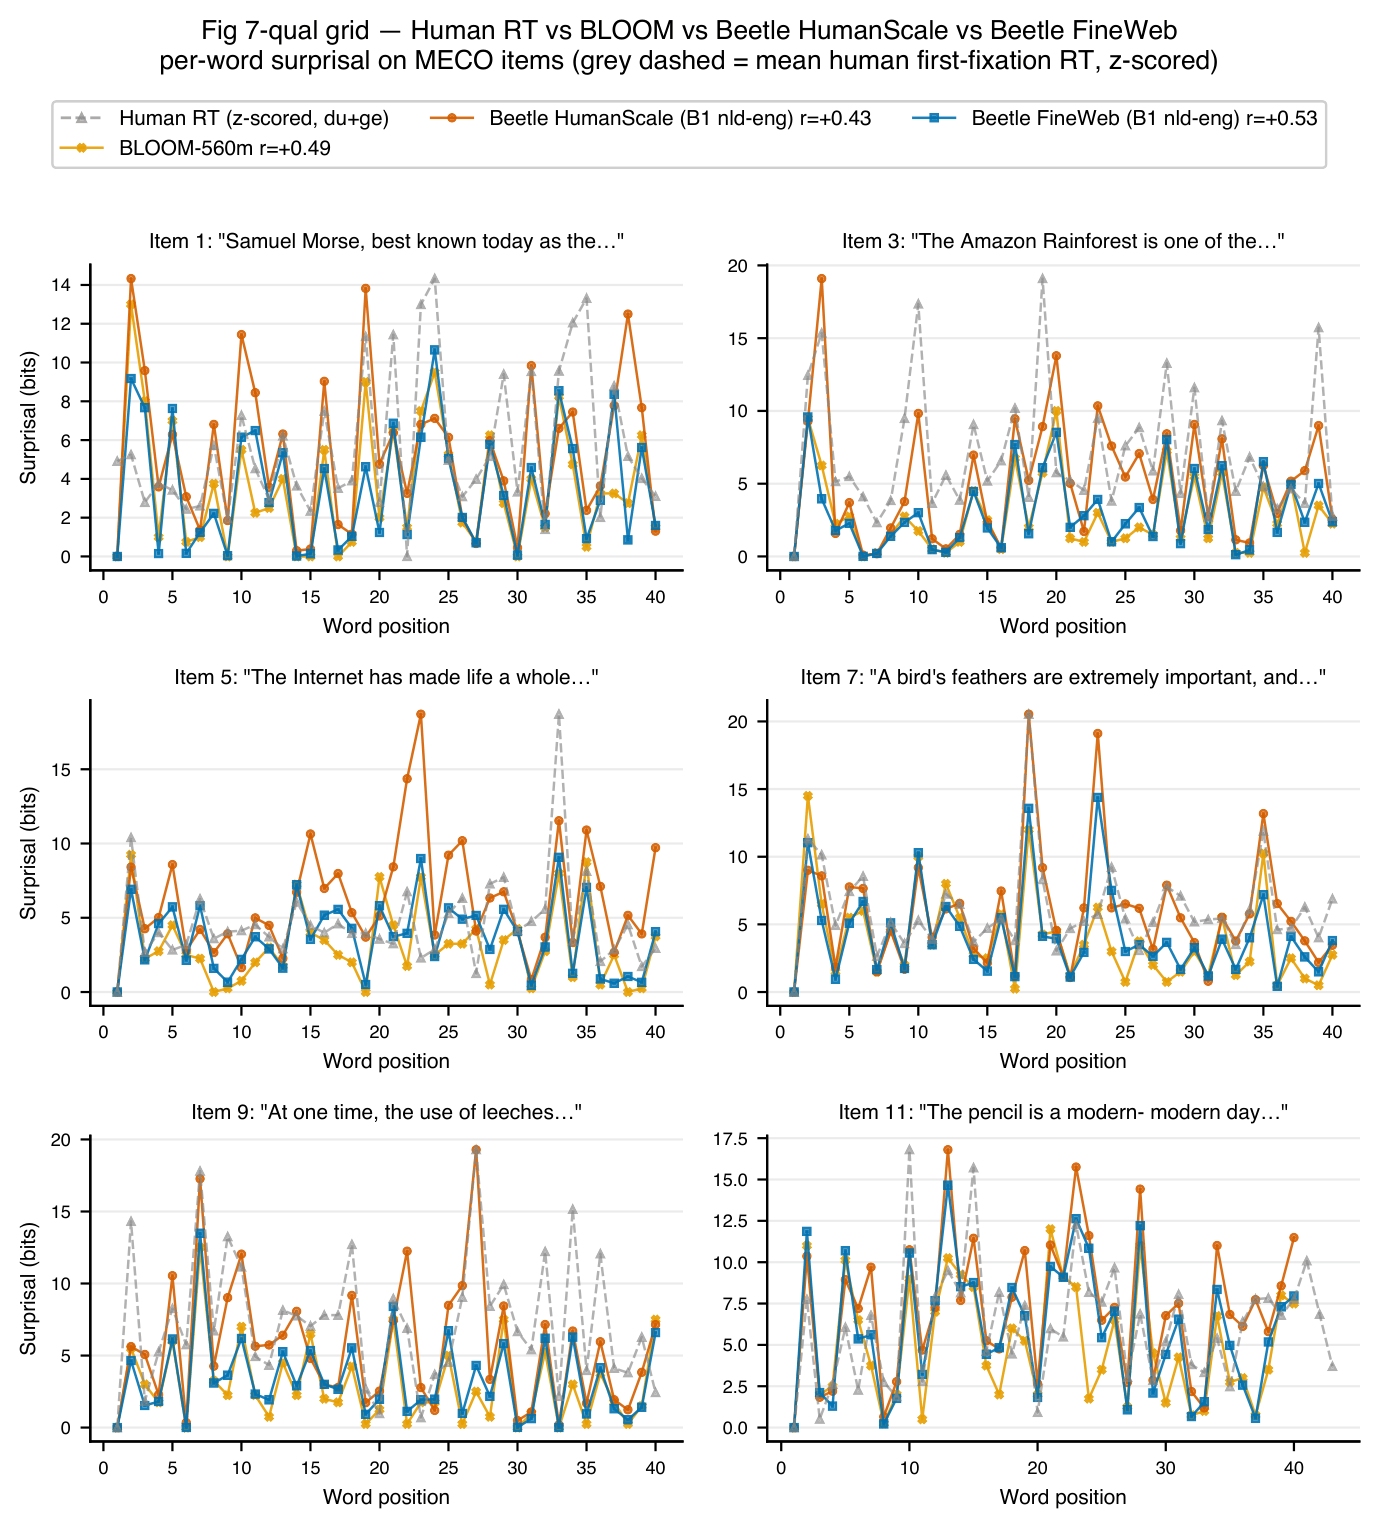
\includegraphics[width=0.5\linewidth]{fig/fig7_qual_grid_bloom_vs_beetle-1.png}
    \caption{Enter Caption}
    \label{fig:placeholder}
\end{figure}
\newpage 

\begin{figure}[!ht]
    \centering
    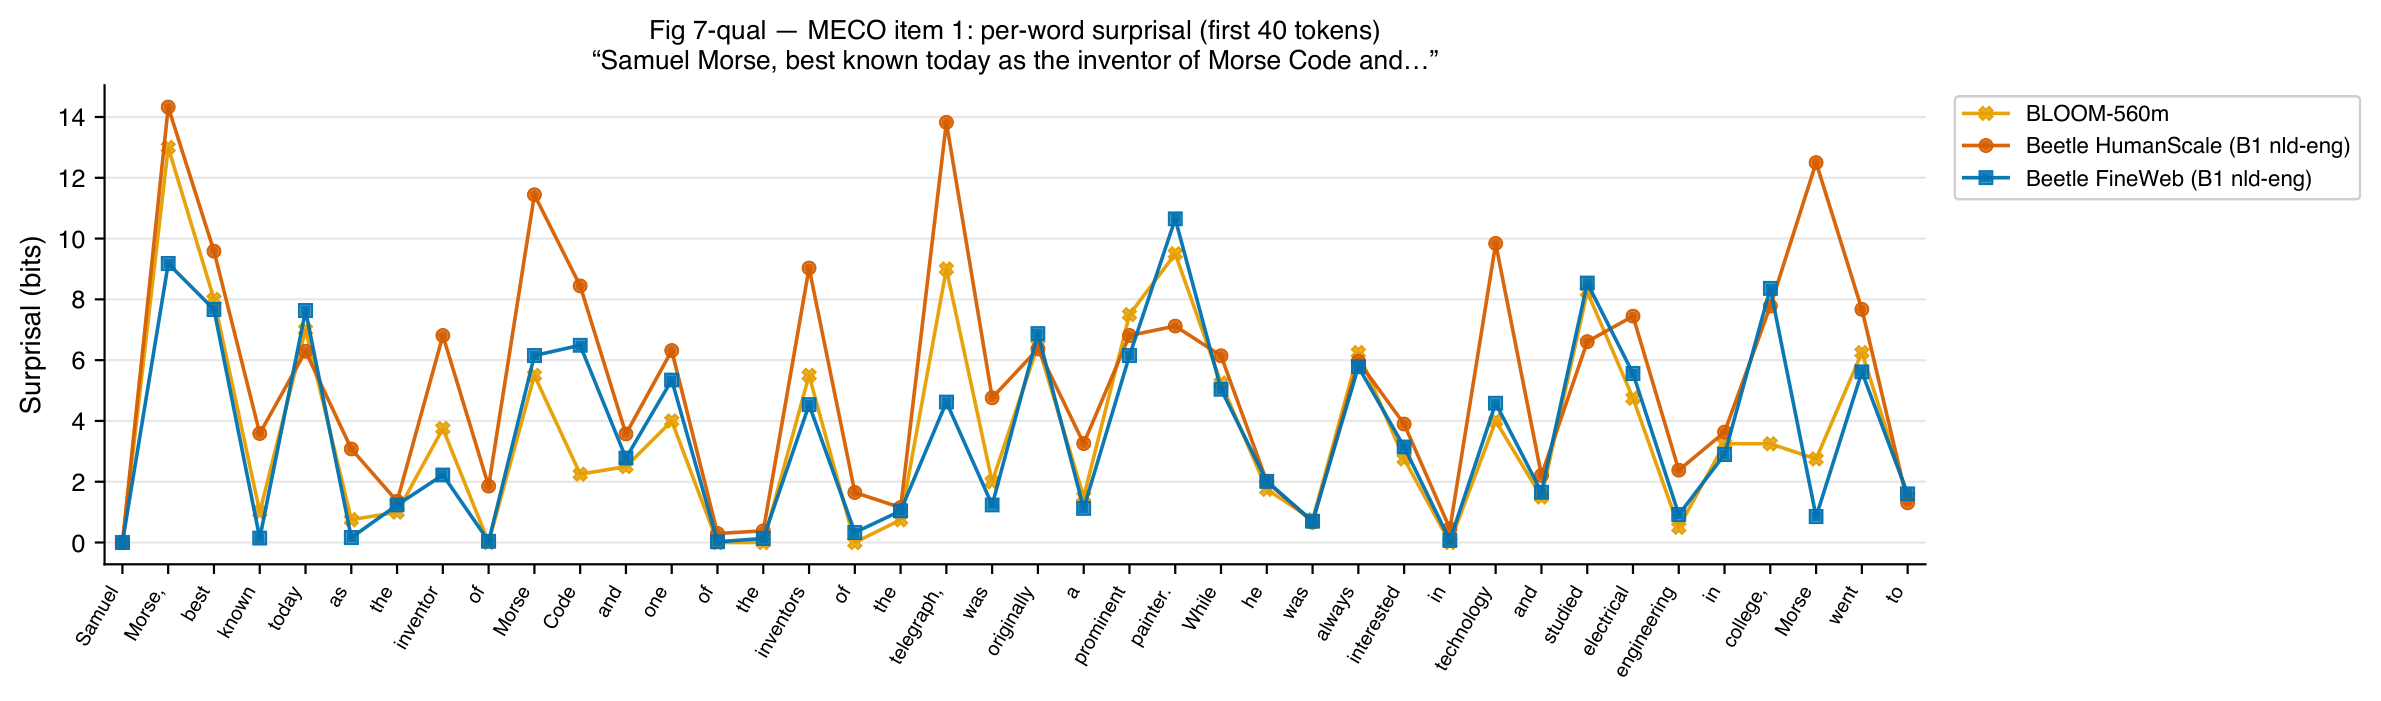
\includegraphics[width=0.51\linewidth]{fig/fig7_qual_item1_bloom_vs_beetle-1.png}
    \caption{Enter Caption}
    \label{fig:placeholder}
\end{figure}
\newpage 

\begin{figure}[!ht]
    \centering
    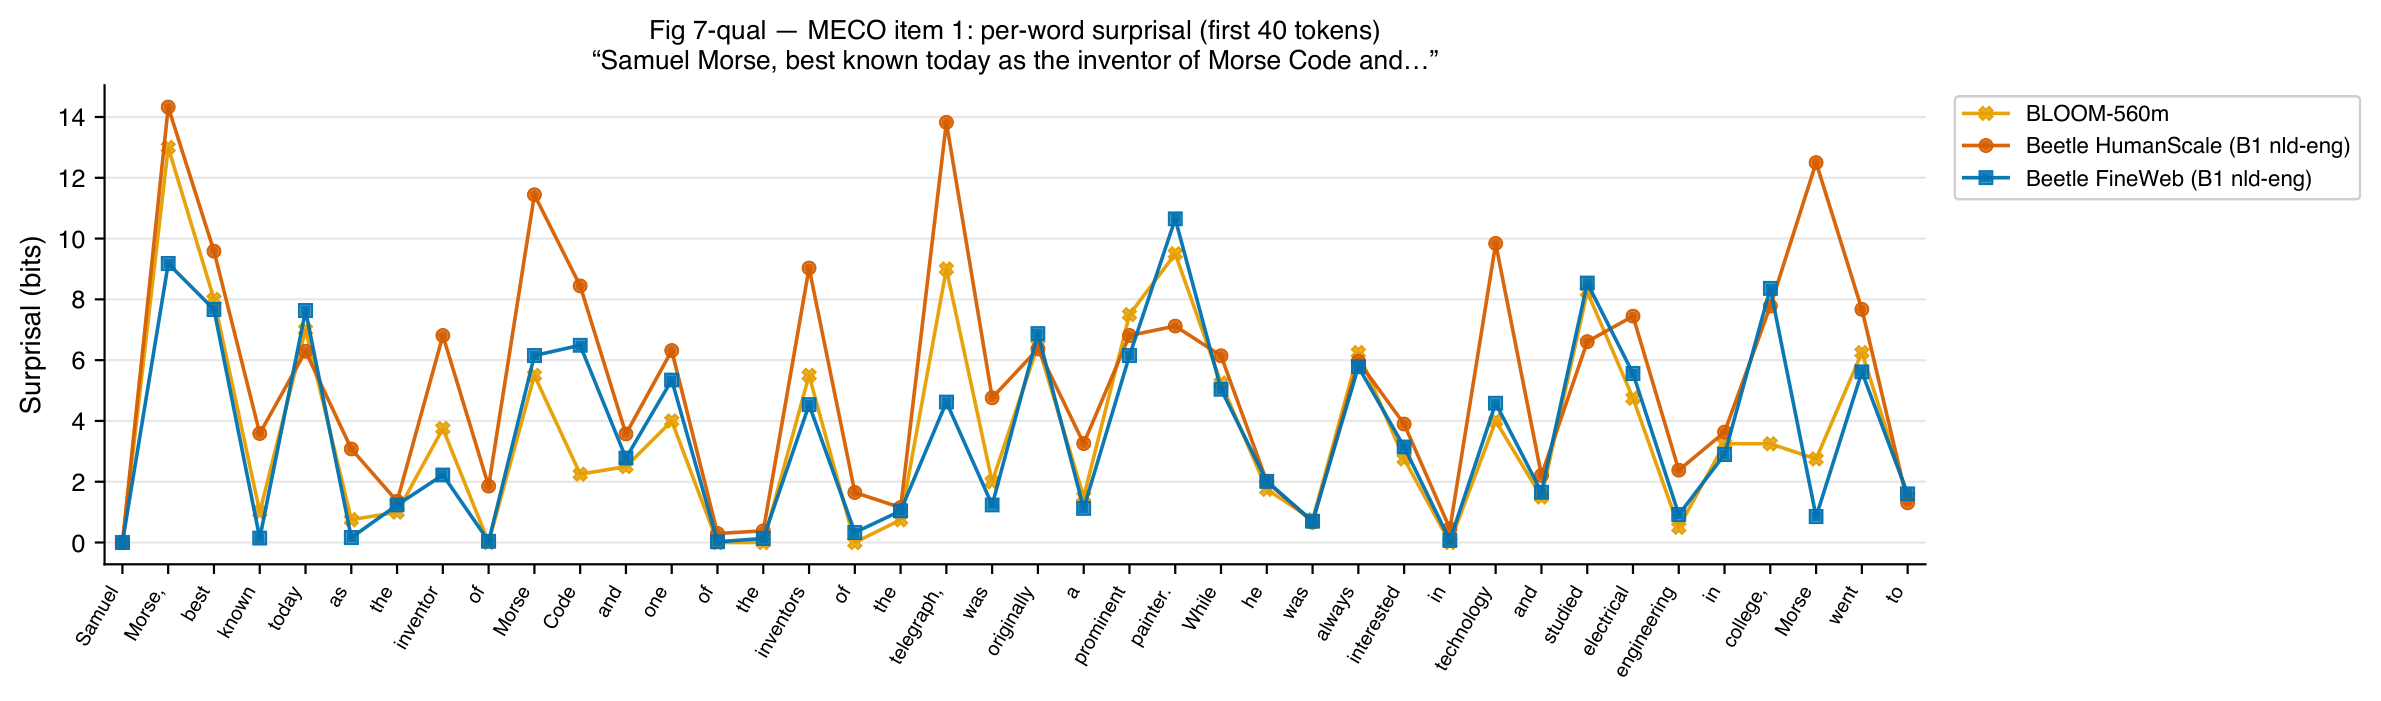
\includegraphics[width=0.5\linewidth]{fig/fig7_qual_item1_bloom_vs_beetle-1.png}
    \caption{Enter Caption}
    \label{fig:placeholder}
\end{figure}

\newpage 

\begin{figure}[!ht]
    \centering
    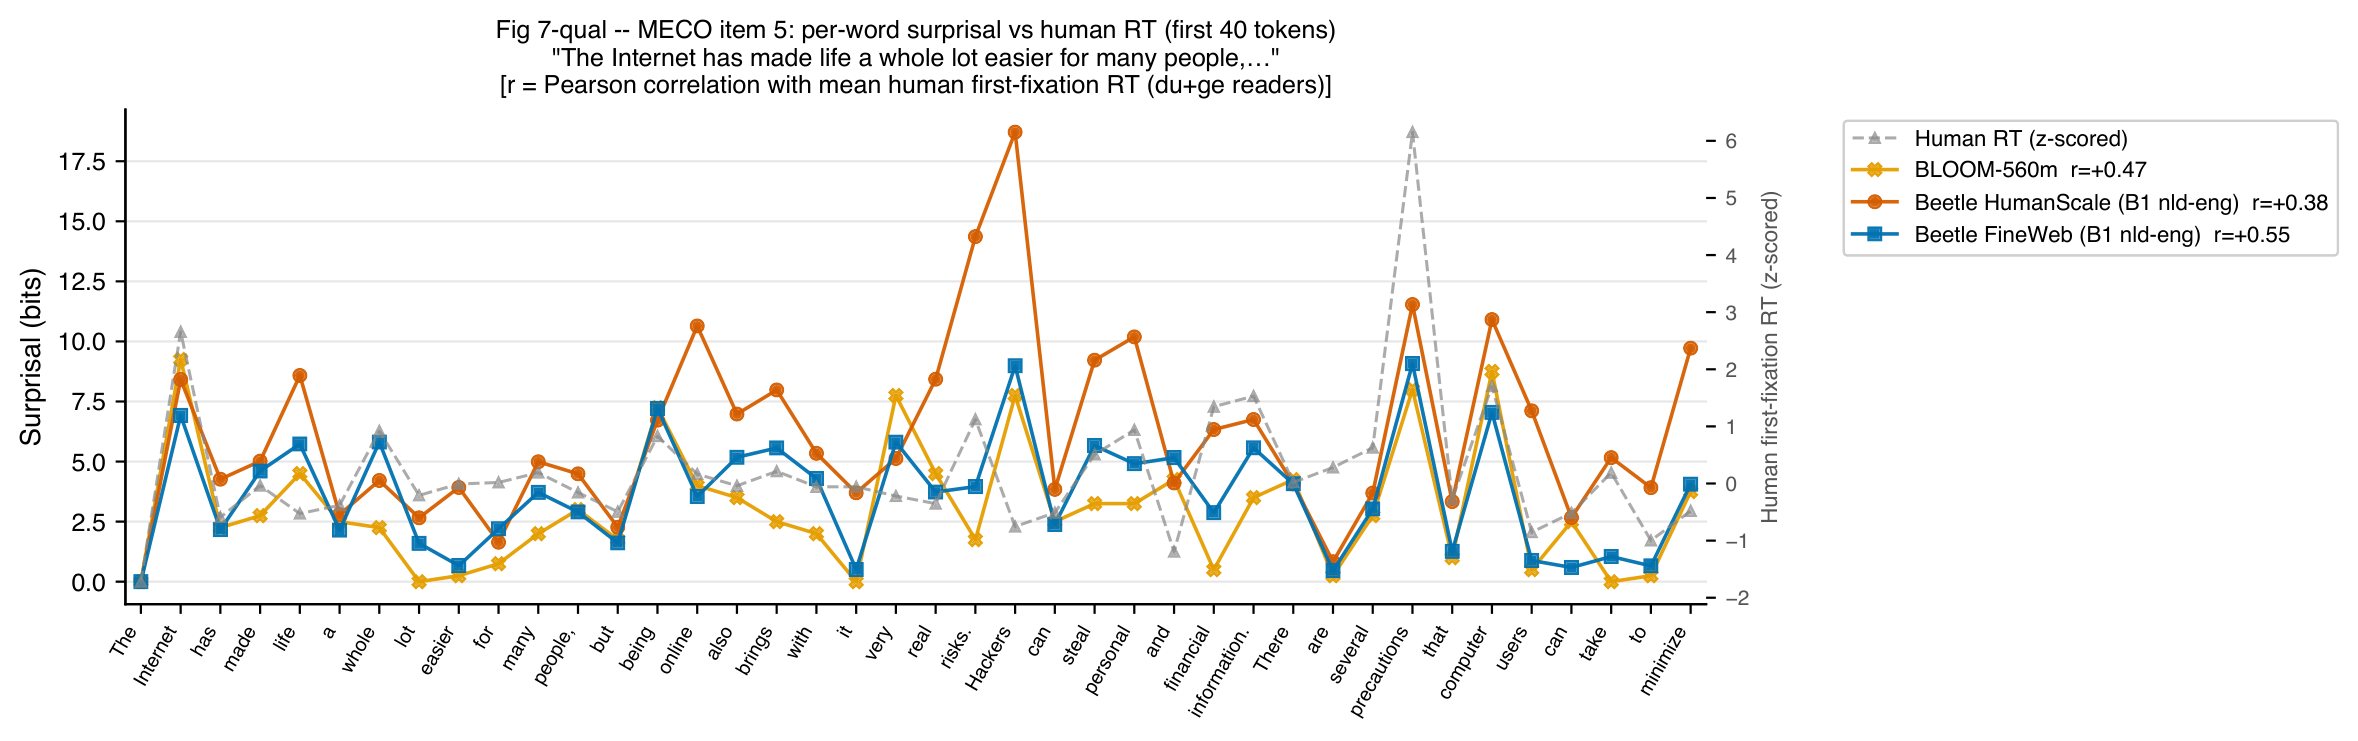
\includegraphics[width=1\linewidth]{fig/fig7_qual_item5_bloom_vs_beetle-1.png}
    \caption{Enter Caption}
    \label{fig:placeholder}
\end{figure}
\newpage 

\begin{figure}[!ht]
    \centering
    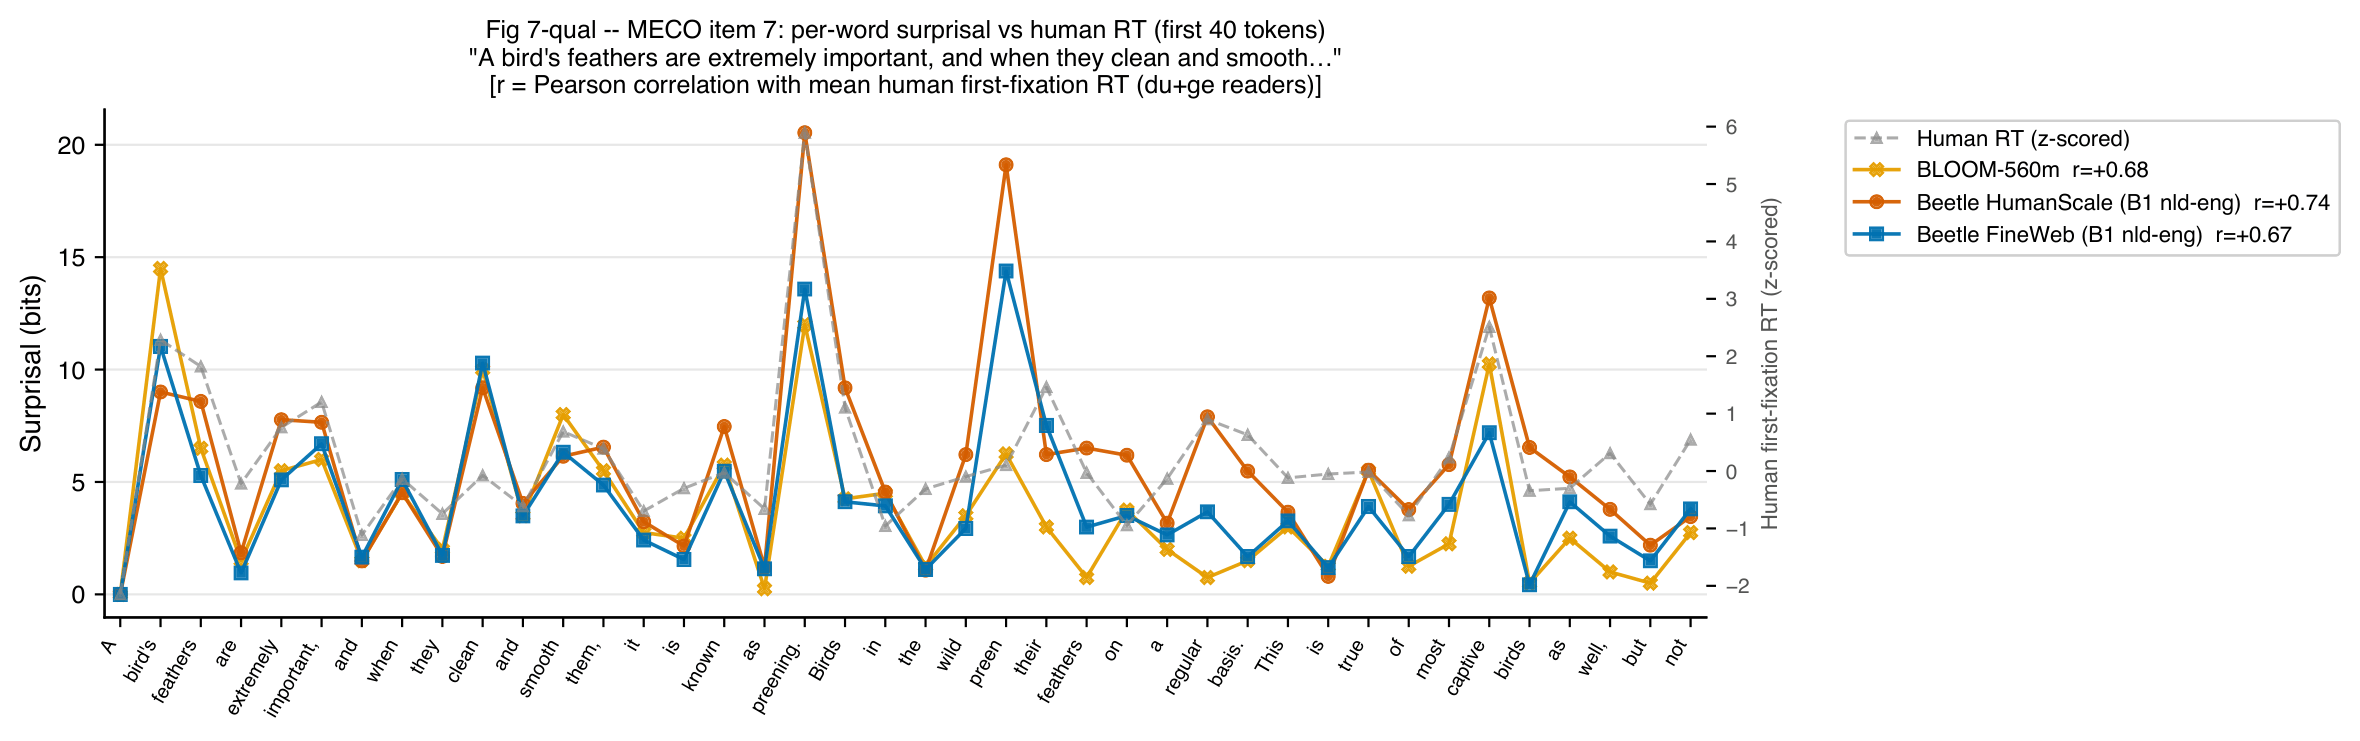
\includegraphics[width=1\linewidth]{fig/fig7_qual_item7_bloom_vs_beetle-1.png}
    \caption{Enter Caption}
    \label{fig:placeholder}
\end{figure}
\newpage 

\begin{figure}[!ht]
    \centering
    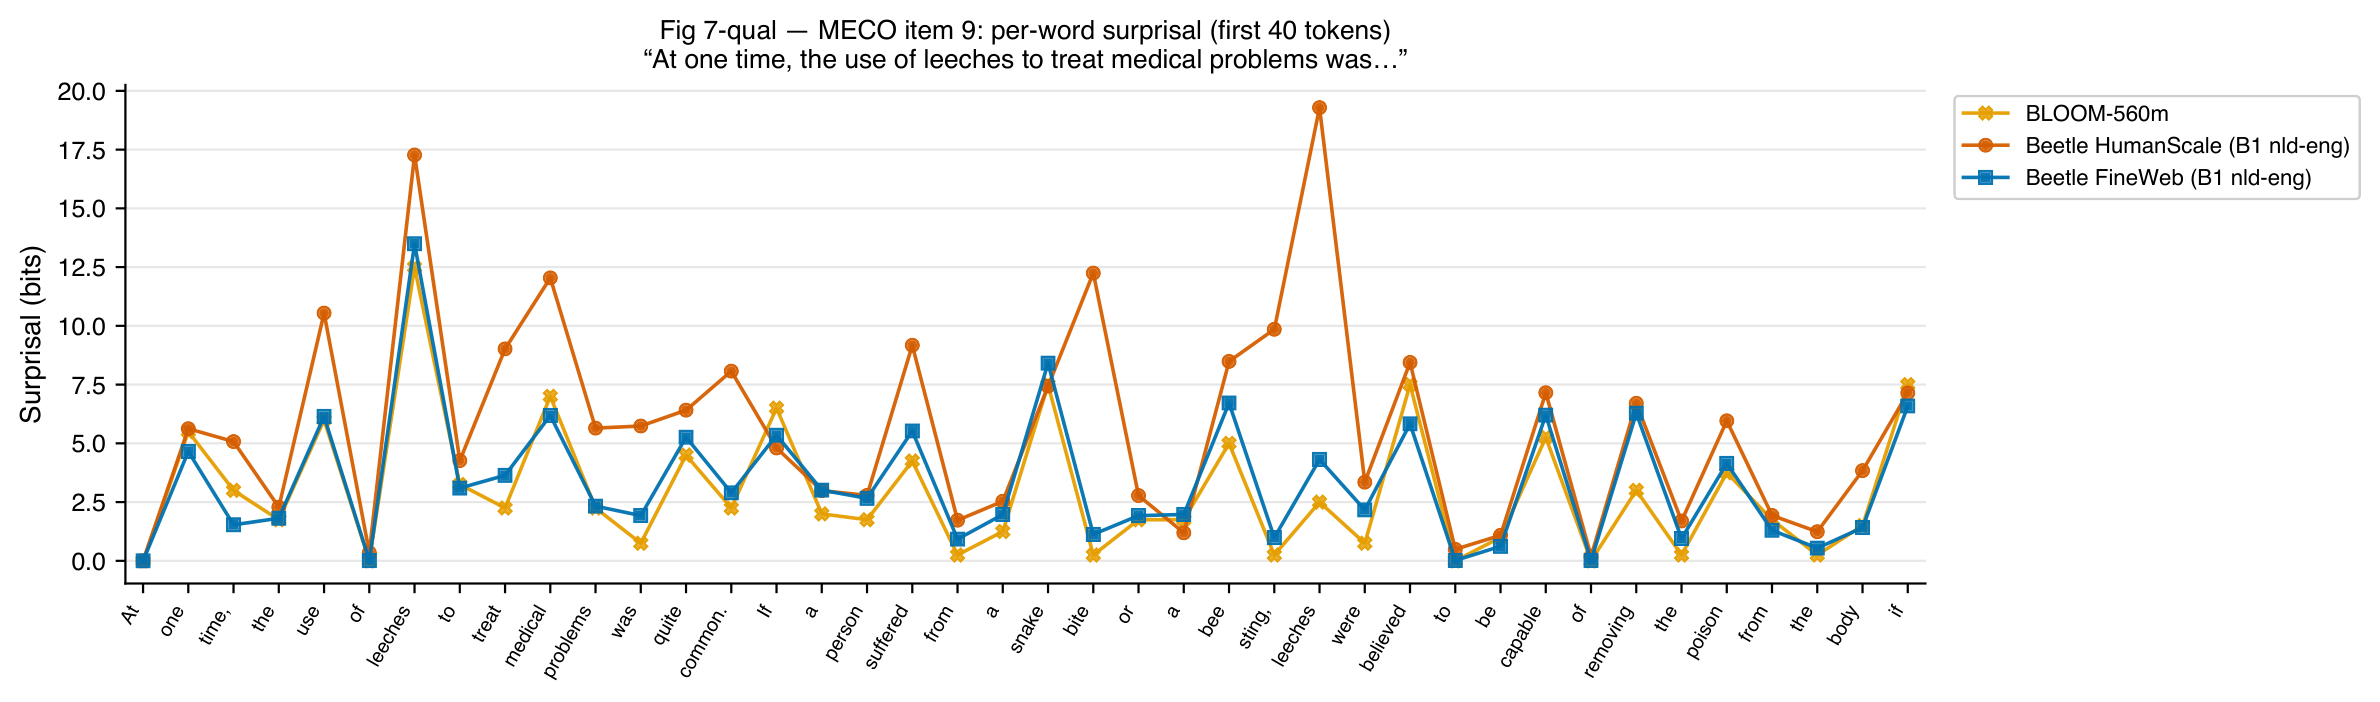
\includegraphics[width=1\linewidth]{fig/fig7_qual_item9_bloom_vs_beetle-1.png}
    \caption{Enter Caption}
    \label{fig:placeholder}
\end{figure}

\newpage 
\begin{figure}[!ht]
    \centering
    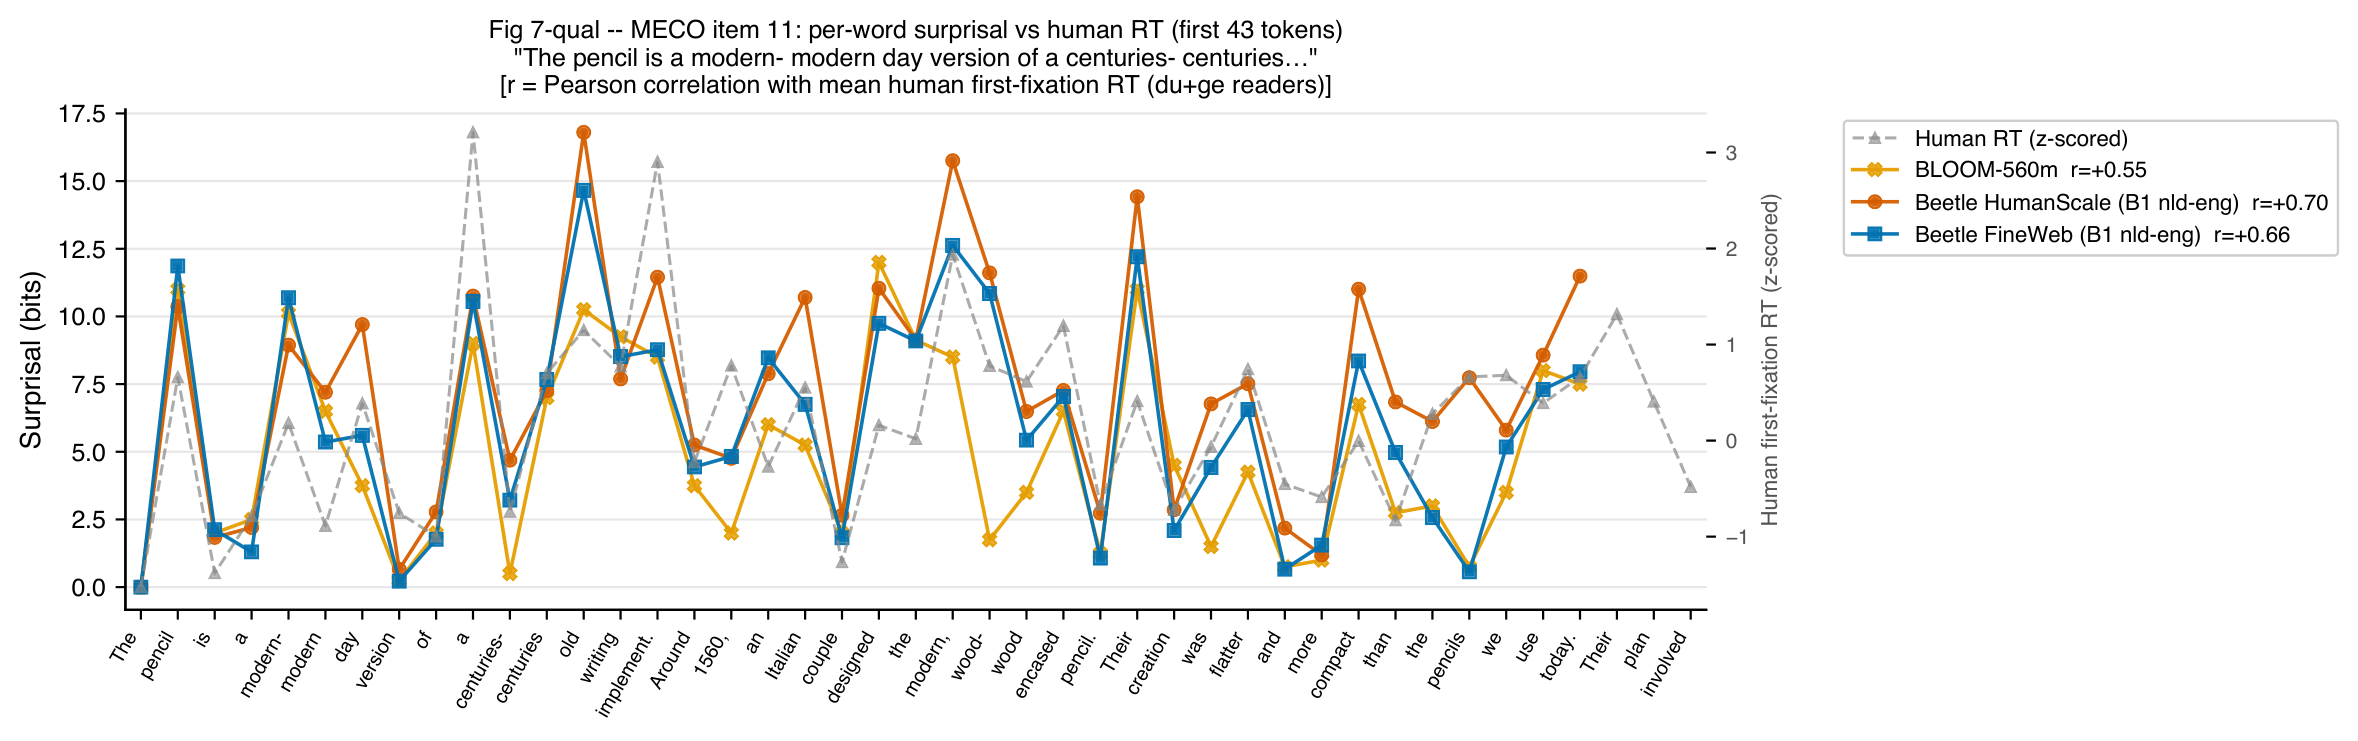
\includegraphics[width=1\linewidth]{fig/fig7_qual_item11_bloom_vs_beetle-1.png}
    \caption{Enter Caption}
    \label{fig:placeholder}
\end{figure}

\newpage 

\begin{figure}[!ht]
    \centering
    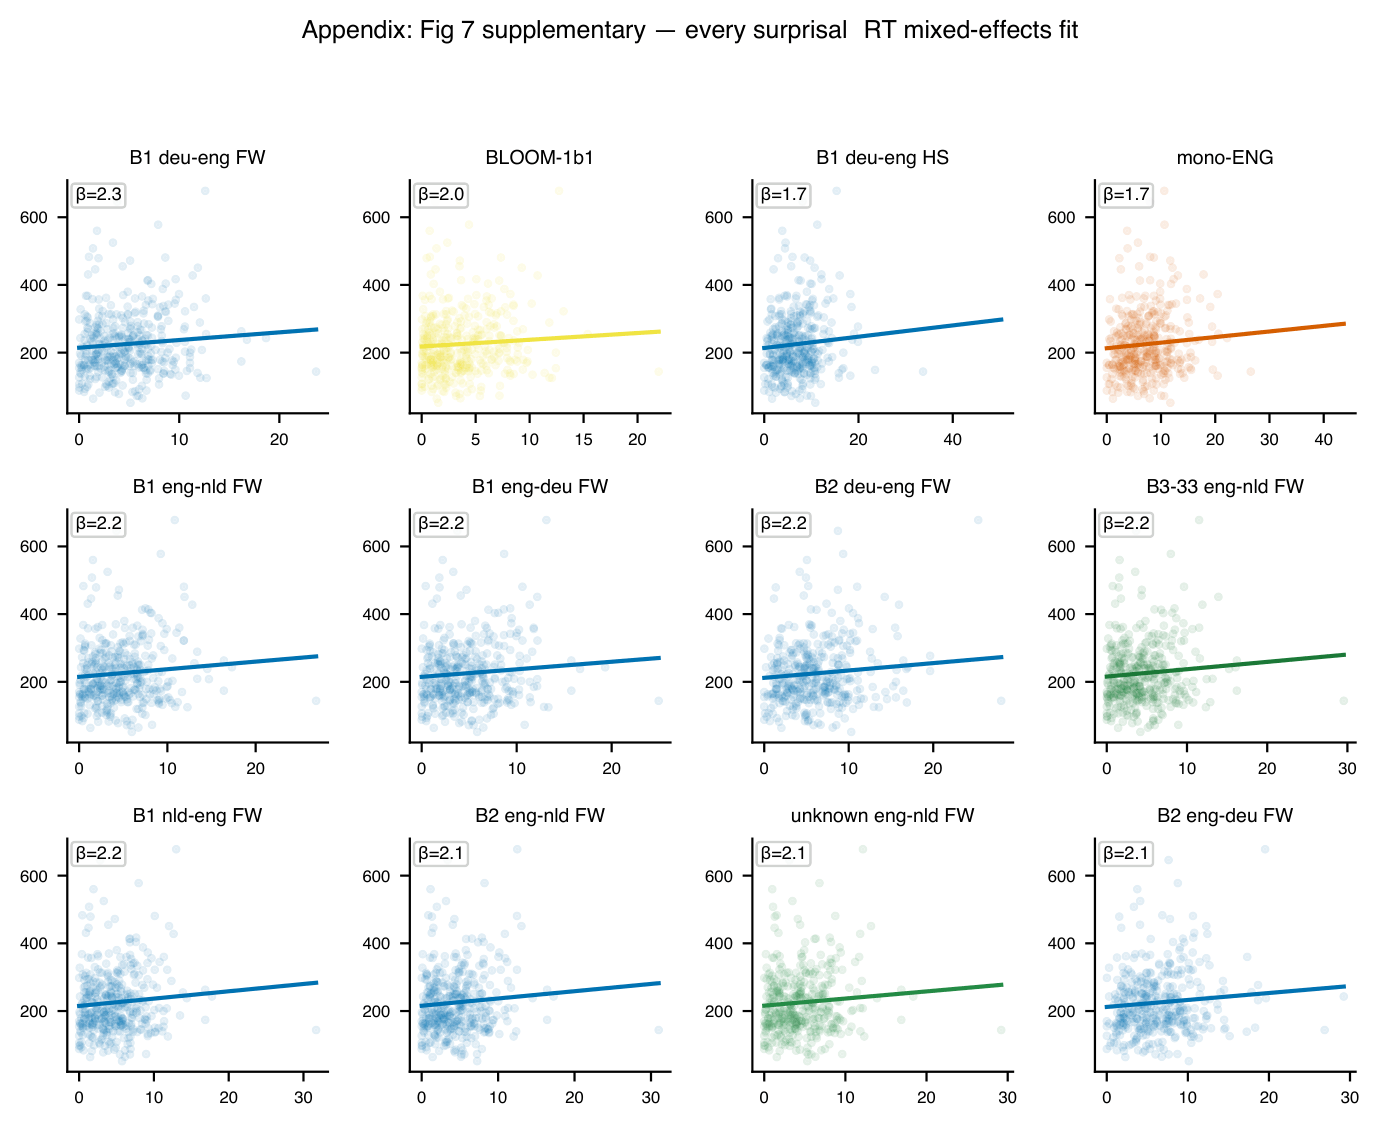
\includegraphics[width=1\linewidth]{fig/fig7_supp_meco_mixed_effects-1.png}
    \caption{Enter Caption}
    \label{fig:placeholder}
\end{figure}

\newpage 
\begin{figure}[!ht]
    \centering
    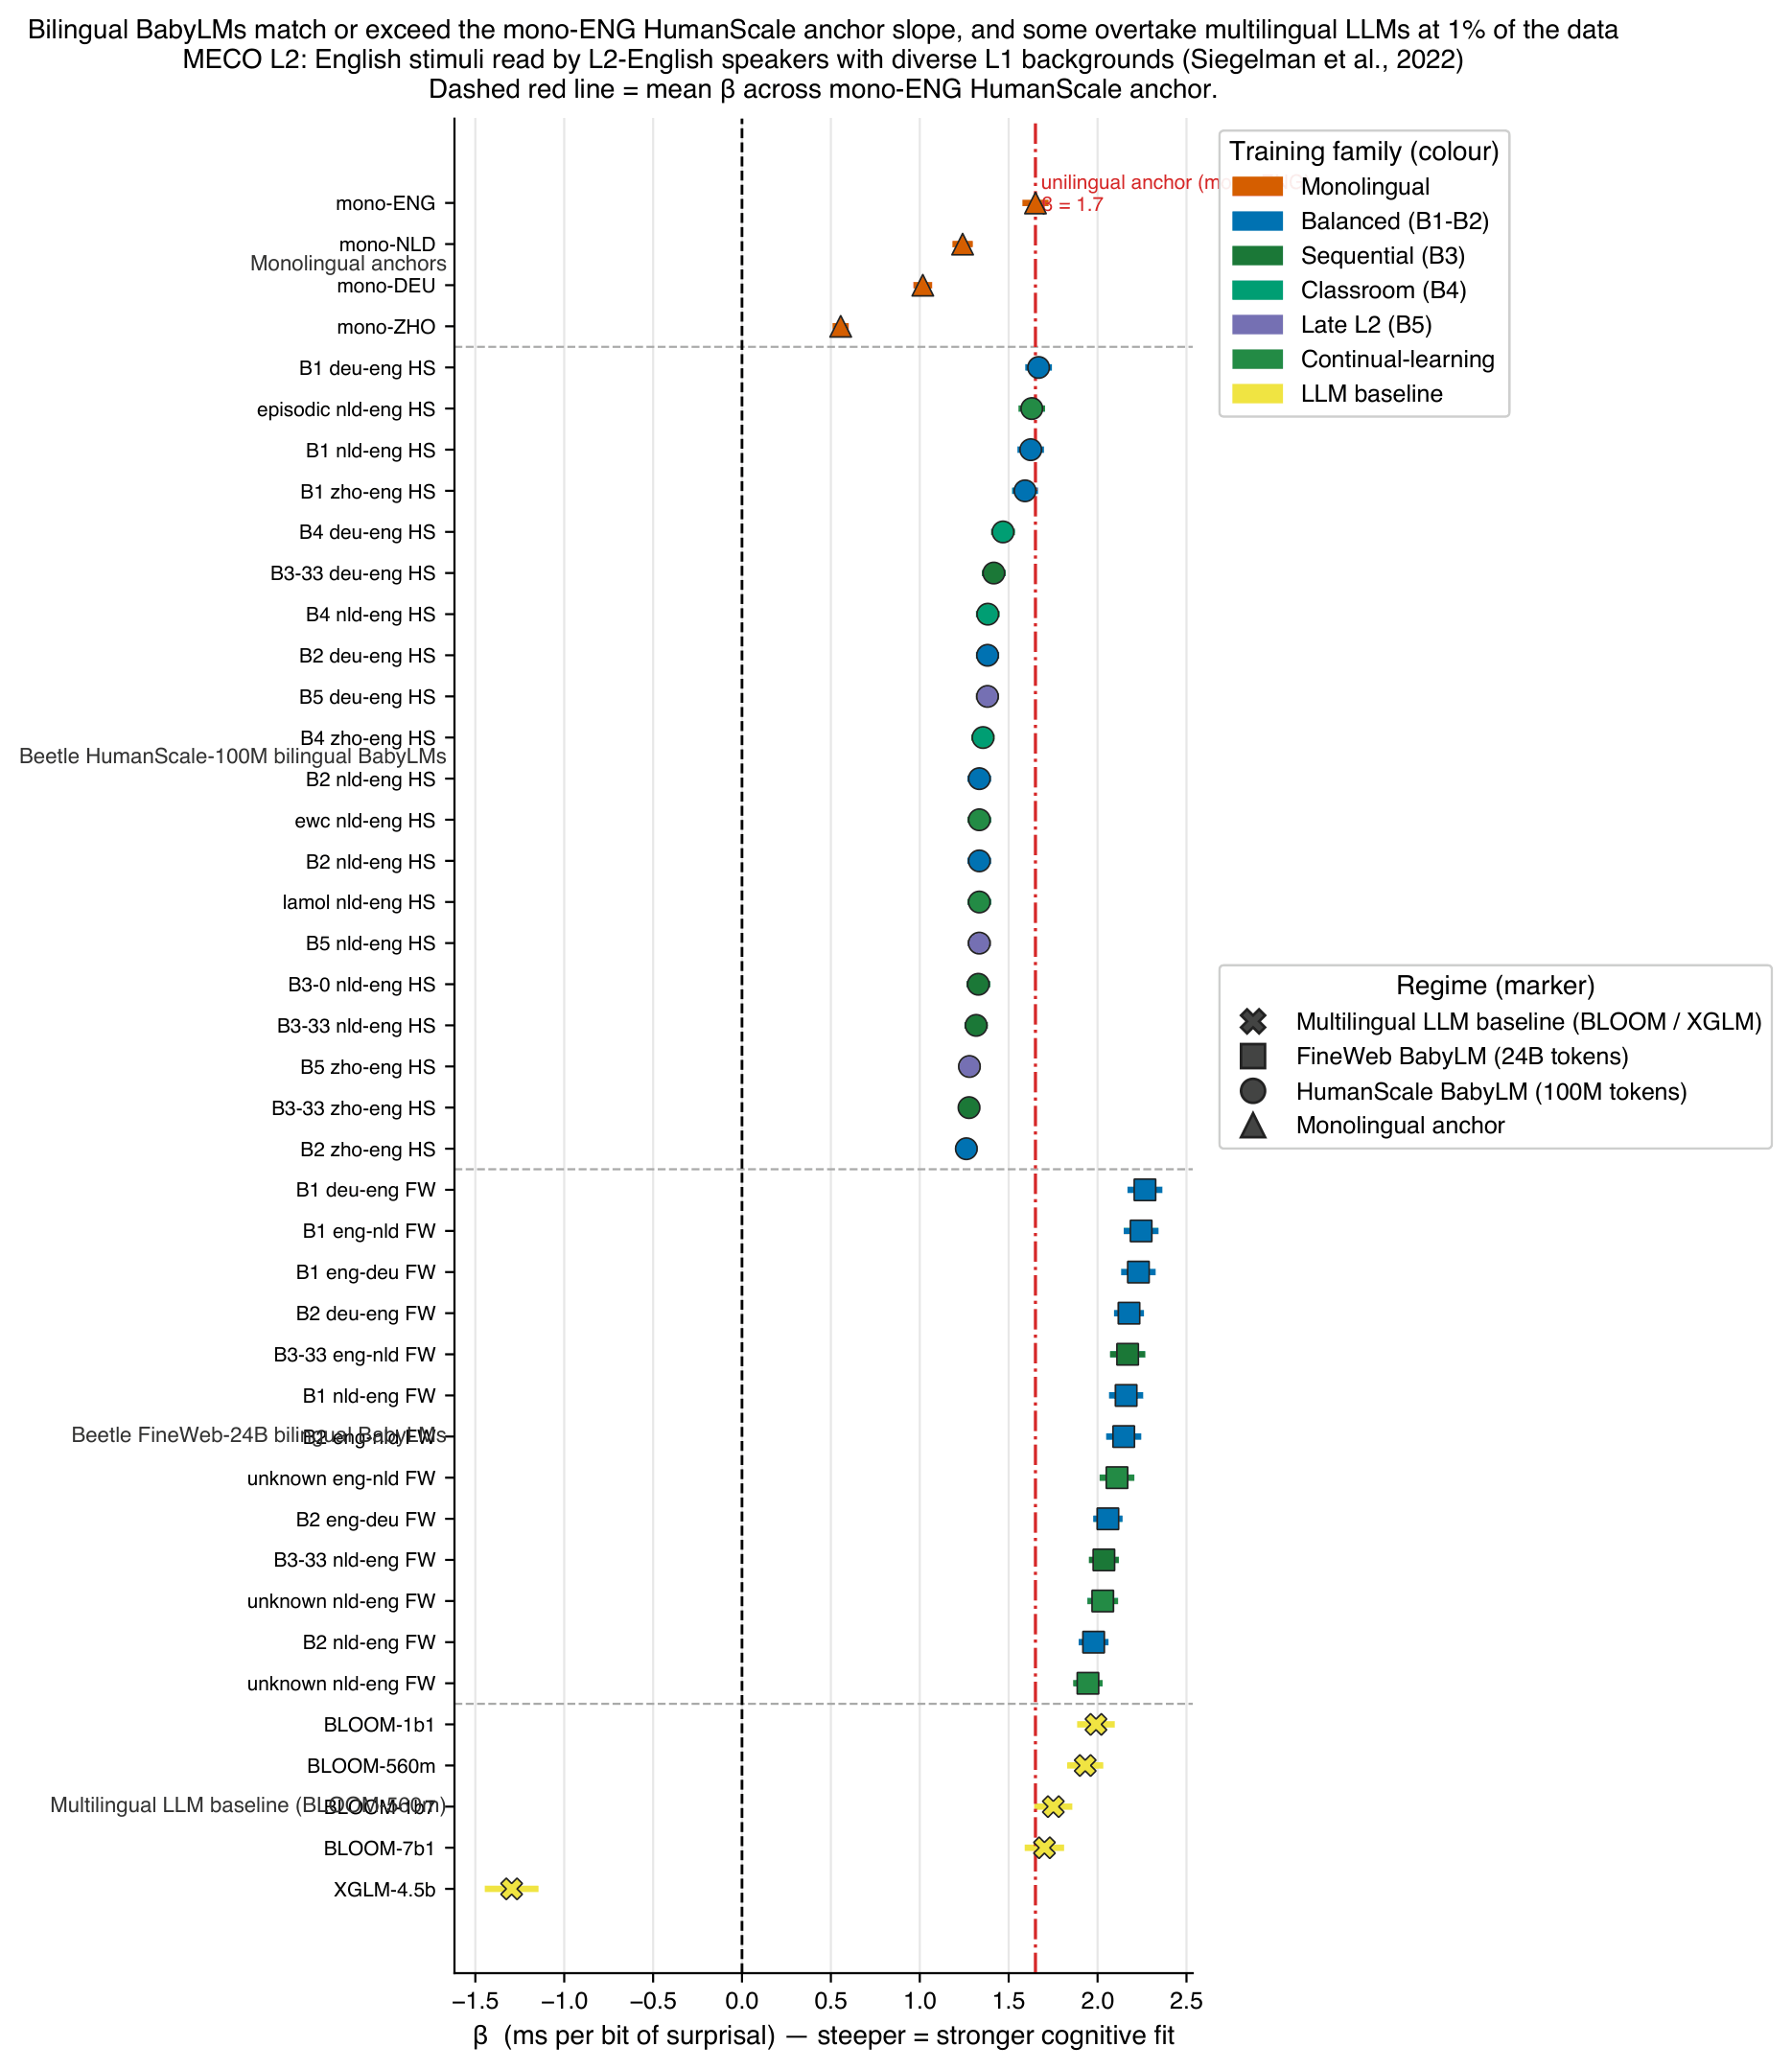
\includegraphics[width=1\linewidth]{fig/fig7b_meco_slope_comparison-1.png}
    \caption{Enter Caption}
    \label{fig:placeholder}
\end{figure}



\newpage 

\newpage 


\section{Literature Review: Comparison between Beetle and other L2LM Training Frameworks} \label{sec:lit-review}

\subsection{Psycholinguistic Tasks}





\suchir{I think our paper is closest to \citet{aoyama2024modeling}, so I want to make comparisons between Beetle and their models much clearer. I don't think the models are available; and also i can't reconstruct the CELER corpus.}



\suchir{Beetle currently implements \textbf{piecewise, phase-based curricula} — a time-structured curriculum that controls exactly which languages (or data sources) a model sees, in what proportions, and at what stages of training. We probably need real exposure shifts gradually, step changes need to be \textit{gradual}. }



\newpage 

\section{\raisebox{-0.3em}{\includegraphics[height=1.2em]{fig/BeetleLM.png}} Training Framework}
\label{sec:train}


In this section, we introduce the training procedure for the Beetle models. 
% We introduce a framework, \raisebox{-0.3em}{\includegraphics[height=1.2em]{fig/BeetleLM.png}}, that formalises multilingual (or polyglot) language acquisition as a complex dynamical system modelled by neural language models under controlled exposure schedules that govern the relative proportion of tokens from two languages throughout training and manipulable control parameters. This formulation treats acquisition as a trajectory in the parameter space, influenced by both input-driven learning and modulating forces. 
We consider multiple curriculum regimes that maintain equal total token budgets across languages but vary the temporal ordering of exposure. This design allows isolation of the effect of exposure timing independent of total data quantity. To enable developmental/longitudinal interpretability analysis, we employ dense training instrumentation using the \textit{pico-train} framework. Models are checkpointed at regular token intervals, storing model parameters, optimisation states and hidden activations. 
\catherine{I think there's been a miscommunication about the checkpointing. I want to do log scale checkpointing like Pythia, not the way that it has been done so far. Regular checkpointing (every 1k steps) doesn't give us sufficient granularity at critical points in the training.}




\begin{table*}[t]
\centering
\small
\setlength{\tabcolsep}{3.5pt}
\begin{tabular}{llll}
\toprule
\textbf{Category} & \textbf{Method} & \textbf{Mechanism} & \textbf{Key Hyperparameters} \\
\midrule

\multicolumn{4}{l}{\textit{Continual Learning \& Replay}} \\

EWC & Elastic Weight Consolidation 
& Quadratic penalty using diagonal Fisher at phase boundary 
& $\lambda$ (0--40), n\_fisher\_samples, trigger \\

MAML / SMLMT & Meta-learning 
& Inner-loop adaptation on support/query splits; outer loss through adaptation 
& hybrid\_ratio (0--0.4), n\_way, k\_shot, inner\_steps \\

LAMOL & Generative replay 
& Pseudo-sample generation from pre-phase model (nucleus sampling) 
& $\lambda_{replay}$ (0--0.5), replay\_ratio, temperature, top\_p \\

Similarity Replay & InsCL-style replay 
& Replay weighted by cross-task similarity (cosine/Wasserstein) 
& similarity\_metric, centroid\_layer, buffer\_size, threshold \\

TILT & Transformer freezing 
& Freeze transformer blocks; train embeddings + LM head only 
& trainable\_modules, reset\_embeddings \\

Exposure LR & Plasticity scheduling 
& Token-exposure-based LR with phase-transition boost 
& plasticity\_boost (1--3), warmup\_tokens, decay\_shape \\

\midrule

\multicolumn{4}{l}{\textit{Curriculum Design}} \\

Curriculum Type & Transition smoothness 
& Sigmoid vs. sharp phase transitions 
& type $\in$ \{smooth, strict\} \\

Phase Schedule & L2/L3 timing 
& Late vs. early vs. episodic introduction 
& B2/B3 (50\%), B5 (80\%), B4/B6 variants \\

Token Split & Data balance 
& Bilingual/trilingual allocation ratios 
& 50:50, 80:20, 33:33:33 \\

Vocab Sharing & Tokenizer structure 
& Shared vs. language-specific vocabularies 
& shared, per\_language \\

Compression & Tokenizer objective 
& Frequency-based or weighted compression 
& equal, proportional, weighted \\

LR Sweep & Optimisation sensitivity 
& Peak learning-rate variation 
& learning rate \\

\midrule

\multicolumn{4}{l}{\textit{Architecture \& Working Memory}} \\

ALiBi Scheduler & Dynamic attention bias 
& Time-varying ALiBi slopes across phases 
& mode, initial/final slope, decay\_rate \\

Pre-pretraining & Formal-language warmup 
& Training on synthetic grammar (Shuffle-Dyck) prior to NL 
& steps, num\_symbols, max\_depth, reset\_optimizer \\

\bottomrule
\end{tabular}
\caption{Beetle training manipulations spanning continual learning, curriculum design, and architectural adaptations. All methods are composable within a unified PICO-based training framework.}
\end{table*}





\subsection{Baseline Architecture}

\catherine{We haven't really talked about messing with learning rate at all. Obviously that has interesting ramifications for the plasticity angle that \citet{constantinescu2025investigating} focus on more. For now I think it would be good to talk about what the learning rate is doing relative to the different exposure phase changes. }

 \raisebox{-0.3em}{\includegraphics[height=1.2em]{fig/BeetleLM.png}} uses a custom Pico decoder \citep{diehl-martinez-etal-2025-pico}, a LLAMA-style \cite{touvron2023llama} stack implemented in plain PyTorch. A sequence of $L=12$ decoder blocks receives 2048 input tokens.  Each block performs RMSNorm \cite{zhang2019rms}, grouped-query self-attention \cite{ainslie2023gqa} with rotary position embeddings \cite{su2024rope}, and a SwiGLU feed-forward network \cite{shazeer2020glu} that expands to $4d$ before projecting back to the model width $d$.  Width is the only scale-dependent hyper-parameter: $d\in\{96,384,768,1536\}$ for the tiny, small, medium and large variants.  All models use 12 heads, 4 key–value heads and causal masking \cite{diehl-martinez-etal-2025-pico}.

\subsection{Training Manipulations}

\begin{table}[t]
\centering
\small
\caption{Full range of training manipulations available in \textsc{BeetleLM}.
All manipulations are toggled via YAML blocks and composed through
\texttt{beetle\_trainer.py}. Continual manipulations (a) are swept on top of
the bilingual/trilingual conditions; curriculum manipulations (b) are set at
the condition-generator level; architectural manipulations (c) are optional
inductive-bias overlays.}
\label{tab:beetle-manipulations}
\begin{tabular}{@{}l l l l@{}}
\toprule
Group & Manipulation & Source & Key parameters \\
\midrule
\multicolumn{4}{l}{\textbf{(a) Continual-learning regularisers \& replay}} \\
& EWC                & Kirkpatrick+ 2017       & \texttt{lambda\_}$\in[0,40]$, Fisher snapshot @ phase change \\
& MAML / SMLMT       & Finn 2017; Bansal 2020  & \texttt{hybrid\_ratio}$\in[0,0.4]$, inner steps, $n$-way / $k$-shot \\
& LAMOL gen.\ replay & Sun+ 2020               & \texttt{lambda\_replay}$\in[0,0.5]$, $T$, top-$p$, replay\_ratio \\
& Similarity replay  & InsCL (Wang+ 2024)      & cosine / Wasserstein centroids, buffer size, threshold \\
& TILT               & Papadimitriou 2020      & freeze backbone, train embed + LM head only \\
& Exposure LR / boost& BeetleLM                & \texttt{plasticity\_boost}$\in[1,3]$, per-phase resets \\
\midrule
\multicolumn{4}{l}{\textbf{(b) Curriculum manipulations}} \\
& Phase schedule     & condition code          & B1--B6 / T1--T4 (see Tables~\ref{tab:bilingual-conditions}, \ref{tab:trilingual-conditions}) \\
& Curriculum type    & curriculum config       & \texttt{smooth} vs \texttt{strict} sigmoid at boundary \\
& Token split        & data\_mix               & 50:50, 80:20 (B4), 90+re-exp (B6), 33/33/33 (T1) \\
& Vocab sharing      & tokenizer config        & \texttt{shared} vs \texttt{per\_language} \\
& Tokenizer compress.& tokenizer config        & \texttt{equal} / \texttt{proportional} / \texttt{weighted} \\
& Peak LR sweep      & optimiser config        & \texttt{training.optimization.lr} \\
\midrule
\multicolumn{4}{l}{\textbf{(c) Architectural / working-memory overlays}} \\
& ALiBi scheduler    & CPLM port               & \texttt{linear} / \texttt{exponential} slope decay over training \\
& Pre-pretraining    & michahu/pre-pretraining & Shuffle-Dyck stage-1 before NL stage-2, optional optimizer reset \\
\bottomrule
\end{tabular}
\end{table}


\subsection{Bilingual Exposure Scheduling}
\begin{table}[t]
\centering
\small
\caption{Human-scale and FineWeb bilingual training conditions. All runs share
the \textsc{pico} backbone (14 layers, $d_{\text{model}}{=}768$, 12 heads, 1 KV head,
seq-len 512, 50K BPE vocab). Human-scale: 10K steps, 50M tokens per language
(100M total). FineWeb: 91{,}552 steps ($\approx$1 epoch over 24B tokens),
effective batch 512. $L_1$ token budgets given for the human-scale setup.}
\label{tab:bilingual-conditions}
\begin{tabular}{@{}l l l l l@{}}
\toprule
Code & Name & Schedule & $L_1{:}L_2$ token split & Repo slug \\
\midrule
\textbf{B1} & Balanced      & 50:50 throughout (from step 0)                             & 50M / 50M & \texttt{balanced-b1} \\
\textbf{B2} & Simultaneous  & 100\% $L_1$ until 50\% of training, sigmoid $\to$ 50:50    & 50M / 50M & \texttt{l2-50-simultaneous-b2} \\
\textbf{B3} & Sequential    & 100\% $L_1$ until 50\% of training, then 33:67 $L_1{:}L_2$ & 50M / 50M & \texttt{l2-50-sequential-33-67-b3} \\
\textbf{B4} & Classroom     & Episodic $L_2$ bursts with EWC, 80:20 token budget         & 80M / 20M & \texttt{l2-50-classroom-20-b4} \\
\textbf{B5} & Late          & $L_2$ introduced at 80\% of training                       & 50M / 50M & \texttt{l2-80-late-b5} \\
\bottomrule
\end{tabular}
\label{tab:curricula}

\end{table}



\begin{table}[t]
\centering
\small
\caption{Trilingual conditions (human-scale \textsc{BabyBabel}: 33M tokens per
language, 99M total; FineWeb: 8B per language, 24B total). Configs live under
\texttt{configs/conditions/trilingual/T\{1\-4\}/train\_\{l1\}\_L1-\{l2\}\_L2-\{l3\}\_L3.yaml}
over 18 orderings drawn from $\{\text{deu, eng, nld, zho}\}$.}
\label{tab:trilingual-conditions}
\begin{tabular}{@{}l l l@{}}
\toprule
Code & Name & Schedule \\
\midrule
\textbf{T1} & Simultaneous Trilingual   & $\approx$33/33/33 mixture, context-clustered batches \\
\textbf{T2} & Sequential Trilingual     & $L_1 \to L_2 \to L_3$ via chained sigmoids           \\
\textbf{T3} & Heritage + $L_3$          & $L_1 \to L_2$ dominance $\to L_3$, with $L_1$ re-exposure \\
\textbf{T4} & Dominant $L_2$ + Late $L_3$ & $L_2$ dominant, $L_1$ weak, $L_3$ introduced late  \\
\bottomrule
\end{tabular}
\end{table}


\begin{table}[t]
\centering
\small
\caption{Minimal B1/B2/B3 ablation sweep on the \texttt{nld-eng} human-scale
pair. Eight variants are trained under three a-priori-fixed seeds
$\{13, 42, 97\}$ to support a paired permutation test + Cohen's $d_z$ +
Holm--Bonferroni on the MECO alignment metric
(\texttt{analyze/significance\_ablation.py}). The full script runs all $8\times3$
cells; the delta script (\texttt{seeds\_13\_97}) assumes seed 42 is already
covered and trains only the remaining $8\times2$. Each variant trains on
8$\times$A100 for $\sim$1h. LAMOL variants use $\lambda_{\text{replay}}=0.2$.}
\label{tab:ablation-sweep}
\begin{tabular}{@{}l l l l@{}}
\toprule
Family & Variant & Manipulation (vs.\ base condition)                     & Repo-slug suffix \\
\midrule
B1 & \textbf{B1}        & Base balanced (50:50 throughout)                     & \texttt{balanced-b1} \\
B1 & \textbf{B1b}       & Balanced with delayed $L_2$ onset variant            & \texttt{balanced-b1-delayed} \\
\midrule
B2 & \textbf{B2}        & Base simultaneous (sigmoid ramp from 50\%)           & \texttt{simultaneous-b2} \\
B2 & \textbf{B2\_ewc}   & + EWC regulariser at phase change                    & \texttt{simultaneous-b2-ewc-l\{$\lambda$\}} \\
B2 & \textbf{B2\_lamol} & + LAMOL generative replay ($\lambda=0.2$)            & \texttt{simultaneous-b2-lamol-l20} \\
B2 & \textbf{B2\_lr}    & + LR plasticity boost at $L_2$ onset                 & \texttt{simultaneous-b2-lr-b\{$k$\}} \\
\midrule
B3 & \textbf{B3}        & Base sequential (33:67 after phase transition)       & \texttt{sequential-33-67-b3} \\
B3 & \textbf{B3\_full}  & Sequential with full EWC + MAML + LR stack           & \texttt{sequential-33-67-b3-ewc-\ldots-maml-\ldots-lr-\ldots} \\
\bottomrule
\end{tabular}

\vspace{0.5em}
\begin{tabular}{@{}l l l l l@{}}
\toprule
Script & Seeds trained & Runs & Wall-clock & Manifest \\
\midrule
\texttt{ablation\_minimal\_nld\_eng.sh}           & 13, 42, 97 & $8\times 3 = 24$ & $\sim$24h & \texttt{variants\_manifest.csv} \\
\texttt{ablation\_minimal\_nld\_eng\_seeds\_13\_97.sh} & 13, 97     & $8\times 2 = 16$ & $\sim$16h & \texttt{variants\_manifest\_seeds\_13\_97.csv} \\
\bottomrule
\end{tabular}
\end{table}

\suchir{not sure if the formalisation is helpful; perhaps it is better to lead with a more qualitative description of the curricula? and, probably more of a comparison with the BGPT models to show the difference between Beetle and BGPT + conceptual motivation?}
\catherine{Yes, I think the point is to explain what each curriculum consists of in terms of exposure and how it compares to common language exposure patterns for bilingual people. I don't think this formalization really helps anything. I also don't think we need to explain EWC or meta learning that much, since these are not methods we're proposing. We basically just need a few sentences to explain what they are and then we compare to them. }

We train bilingual causal language models under controlled exposure schedules g. Let \( L_1 \) and \( L_2 \) denote the two training languages. We define an exposure schedule \( \alpha(t) \in [0,1] \), representing the probability that a training example at training step \( t \) is sampled from language \( L_2 \). The complementary probability \( 1-\alpha(t) \) determines sampling from \( L_1 \).


 

Let $\mathcal{L}_1$ and $\mathcal{L}_2$ denote two languages with vocabularies $\mathcal{V}_1$ and $\mathcal{V}_2$ and corpora $\mathcal{D}_1$ and $\mathcal{D}_2$. A \textbf{bilingual language model (BiLM)} parameterized by $\theta$ defines a joint probabilistic model over sequences drawn from either language:
\[
P_\theta(x) =
\begin{cases}
P_\theta(x \mid L_1), & x \in \mathcal{V}_1^* \\
P_\theta(x \mid L_2), & x \in \mathcal{V}_2^*
\end{cases}
\]
The LM is trained under a\textbf{ time-dependent mixture of languages}. Training proceeds over a time-dependent mixture of language data governed by an exposure function $\alpha(t)$, where $t \in [0,T]$ indexes training steps:
\[
\mathcal{D}_{\text{mix}}(t) = \alpha(t)\,\mathcal{D}_1 \cup (1-\alpha(t))\,\mathcal{D}_2.
\]

The objective maximizes log-likelihood over the evolving training distribution:
\[
\theta^* = \arg\max_\theta \sum_{t=1}^{T} \sum_{x \in \mathcal{D}_{\text{mix}}(t)} \log P_\theta(x).
\]
where $\alpha(t) \in [0,1]$ controls L1 exposure at step $t$.

% \paragraph{Configuration via YAML.}
% \raisebox{-0.3em}{\includegraphics[height=1.2em]{fig/BeetleLM.png}} exposure scheduling data curricula are specified declaratively through YAML configuration files. This declares distinct training phases for polyglot language modelling based on a ratio of steps. Within each phase, a custom data mixture can be specified. An example \raisebox{-0.3em}{\includegraphics[height=1.2em]{fig/BeetleLM.png}}  YAML configuration can be found in \autoref{}


\subsection{Polyglot Language Exposure Curricula}


We can generalise our formulation to treat multilingual or polyglot acquisition as a controlled variation in training distribution over time. To model multilingual acquisition scenarios during training, we represent language exposure as a time-varying distribution over languages. 
Let $N$ denote the number of languages and $t \in [0,T]$ the training progress. 
We define a \textit{language exposure vector}

\[
\boldsymbol{\alpha}(t) = (\alpha_1(t), \alpha_2(t), \dots, \alpha_N(t)),
\]

where $\alpha_i(t)$ denotes the proportion of training tokens drawn from language $L_i$ at time $t$. 
The exposure vector forms a probability distribution over languages:

\[
\sum_{i=1}^{N} \alpha_i(t) = 1.
\]

During training, batches are sampled according to the exposure vector $\boldsymbol{\alpha}(t)$, allowing the language mixture to vary dynamically as training progresses. This formulation generalizes bilingual curricula to trilingual and polyglot settings, enabling controlled experiments over multilingual acquisition schedules.

The model parameters $\theta$ are trained to maximise the likelihood of sequences drawn from this evolving distribution:

\[
\theta^* = \arg\max_\theta 
\sum_{t=1}^{T} 
\sum_{x \sim \mathcal{D}_{\text{mix}}(t)}
\log P_\theta(x).
\]


\subsection{Control Parameters}

Sequential multilingual training exposes models to a well-documented failure mode: as the model acquires a new language, gradient updates systematically overwrite the weight configurations that supported the previously learned language, a phenomenon known as catastrophic forgetting \citep{mccloskey1989catastrophic,kirkpatrick2017overcoming}. This problem is particularly acute under the \texttt{sequential} curriculum, where L1, L2, and L3 phases are presented in strict succession with no interleaving, maximising the distributional shift experienced at each phase boundary.  We  define \textbf{control parameters}, $\mathbf{F}_t$, The parameter update at each training step of the polyglot language model defines the system's dynamics:
\begin{equation}
\theta_{t+1} = \theta_t - \eta \, \mathnormal{\nabla}_{\theta} \mathcal{L}_t(\theta_t; \mathcal{D}_{\mathrm{mix}}(t)) + \mathbf{F}_t
\end{equation}
where $\eta$ is the learning rate, $\mathcal{L}_t$ is the training loss on the mixed data.

\subsubsection{Elastic Weight Consolidation}

Elastic Weight Consolidation (EWC) is a parameter-regularization approach to continual learning that mitigates forgetting by discouraging large changes to parameters that are important for previously learned tasks \citep{kirkpatrick2017overcoming}.  In a sequential bilingual learning setting, suppose $\theta^*$ denotes parameters learned after training on $\mathcal{D}_1$. When subsequently training on $\mathcal{D}_2$, EWC modifies the loss function:

\[
\mathcal{L}_{\text{EWC}}(\theta)
= \mathcal{L}_{2}(\theta)
+ \lambda \sum_{i} F_i (\theta_i - \theta_i^*)^2,
\]

where $F_i$ denotes the Fisher information matrix estimated via Monte Carlo on $K\!=\!10$ held-out L1 batches:
\begin{equation}
    \hat{F}_i
    = \frac{1}{K}\sum_{k=1}^{K}
      \left(\frac{\partial\log p(x_k\mid\theta)}{\partial\theta_i}\right)^{\!2}.
    \label{eq:fisher}
\end{equation}
The snapshot of $\theta^*$ and the Fisher computation are triggered
automatically at curriculum phase boundaries. The Fisher information matrix measures the importance of parameter $\theta_i$ to the first task and $\lambda$ controls the strength of regularization. The additional penalty constrains parameter updates during L2 training, preserving performance on L1.  \citet{constantinescu2025investigating} use EWC to address catastrophic forgetting by introducing an explicit stability constraint in parameter space, rather than modifying the training distribution.

\subsubsection{Meta-Learning for Cross-Lingual Adaptation}
While exposure schedules $\alpha(t)$ control the \emph{distributional trajectory} of multilingual input, they do not directly shape the \emph{adaptation dynamics} of the model, often resulting in a \textit{stability--plasticity} dilemma where standard gradient descent fails to reconcile rapid language shifts (e.g., L1 $\rightarrow$ L2) with the retention of previously acquired structures. To mitigate this, meta-learning serves as a complementary control mechanism $\mathbf{F}_t$ that operates on the learning process itself, biasing the parameter trajectory toward initializations $\theta$ that support rapid task adaptation and minimize expected loss after minimal updates. Within the \raisebox{-0.3em}{\includegraphics[height=1.2em]{fig/BeetleLM.png}} framework, this approach reshapes the loss landscape to promote representations that are both reusable and rapidly reconfigurable, specifically through an optional (First-Order) Model-Agnostic Meta-Learning (MAML) configuration integrated into pretraining. Following the Subset-Mask Language Modelling (SMLMT) paradigm \cite{bansal-etal-2020-self, africa-etal-2025-learning, africa-etal-2025-meta}, the model interleaves autoregressive updates with meta-episodes where disjoint support and query positions are sampled to construct $N$-way classification tasks; during these episodes, a lightweight classifier head is adapted via inner-loop SGD steps while the backbone remains frozen, after which an outer loss is computed on the query set to allow gradients to flow through the backbone and optimize for rapid adaptation. By tuning task entropy through $N$-way, $K$-shot episodes and controlling the frequency of meta-updates via a hybrid ratio, this method systematically exposes the model to structured few-shot generalization, ensuring robust performance across the evolving exposure regimes and constrained data budgets typical of polyglot acquisition.

\subsection{Dense Checkpointing and Instrumentation}

\raisebox{-0.3em}{\includegraphics[height=1.2em]{fig/BeetleLM.png}} builds on the \textbf{Pico} training and learning dynamics framework \citep{diehl-martinez-etal-2025-pico}, 

%We store at regular token intervals:
%\begin{itemize}
%    \item Model parameters and optimizer states.
%    \item Hidden activations on evaluation datasets.
%    \item Gradient statistics and training metadata.
%\end{itemize}
%This enables analysis of representational formation, neuron specialization, and parameter reuse over time.

\paragraph{Checkpointing}  \raisebox{-0.3em}{\includegraphics[height=1.2em]{fig/BeetleLM.png}} implements a curriculum-aware checkpointing framework for bilingual language model training. Curricula are defined along two independent axes: the point at which a new language – the second language (L2) –  is introduced and its relative proportion within each phase.  Checkpoints are automatically triggered both at fixed intervals and immediately upon phase transitions, ensuring particularly dense checkpointing at the introduction of a new language in pretraining, enabling fine-grained analysis of bilingual acquisition dynamics. Each checkpoint records the model parameters, optimizer and scheduler states, pipeline state, evaluation results, and optionally learning dynamics, supporting reproducibility and phase-aware comparisons across curricula.
\catherine{Is this what's happening though because on the models on HF, I see checkpointing every 1k steps?}


\subsection{Tokenization}

\raisebox{-0.3em}{\includegraphics[height=1.2em]{fig/BeetleLM.png}} contains modular logic for tokenization logic, allowing investigation of 
% the benefits of vocabulary overlap \citep{kallini-etal-2025-false} and 
different tokenization schemes (e.g., SentencePiece, UnigramLM, SuperBPE, BPE).  In our training framework, tokenizers are trained on a proportional data mix with equal compression, so the model see the amount of information for each language in each sequence. All reported experiments utilise BPE tokenization. \textbf{Monolingual tokenizers} are trained from scratch on 2M tokens
drawn uniformly from the target language, matching the total corpus budget used
by bilingual tokenizers (1\,M L1 + 1\,M L2). \textbf{Bilingual tokenizers} are trained jointly on one language pair and shared across both L1$\to$L2 and L2$\to$L1 orderings. \textbf{Trilingual} experiments reuse a single pre-trained trilingual tokenizer to avoid vocabulary confounds in the catastrophic forgetting analyses. Vocabulary sizes are set to \textbf{32{,}000} for monolingual models and
\textbf{32{,}768} for bilingual and trilingual models, the additional capacity
accommodating the larger type inventory of multi-language vocabularies.
\catherine{1) how much data is the tokenizer trained on 2) how did we choose vocab size/same vocab size for mono/bi-/trilingual?}






\subsection{Default \raisebox{-0.3em}{\includegraphics[height=1.2em]{fig/BeetleLM.png}} Training Configurations}

All models use the \textbf{PicoDecoder} architecture---a decoder-only causal
Transformer with Grouped-Query Attention (GQA)~\citep{ainslie2023gqa}.
Architecture hyperparameters are shared across all experimental conditions and
listed in Table~\ref{tab:default_configs}.

\begin{table*}[h!]
\centering
\small % Slightly smaller font to ensure fit
\renewcommand{\arraystretch}{1.3}
\begin{tabular}{@{} l l l @{}}
\toprule
\textbf{Category} & \textbf{Parameter} & \textbf{Default Value} \\
\midrule
\multirow{9}{*}{\textbf{Model}}
 & Model Type & \texttt{pico\_decoder} \\
 & Hidden Dimension ($d_{\text{model}}$) & 768 \\
 & Number of Layers ($n_{\text{layers}}$) & 12 \\
 & Vocabulary Size & 50,304 \\
 & Sequence Length & 2,048 \\
 & Attention Heads & 12 \\
 & Key/Value Heads & 4 \\
 & Normalization Epsilon & $1 \times 10^{-6}$ \\
 & Positional Embedding Theta & 10,000.0 \\
\midrule
\multirow{7}{*}{\textbf{Training}}
 & Optimizer & AdamW \\
 & Learning Rate & $3 \times 10^{-4}$ \\
 & LR Scheduler & Linear w/ Warmup \\
 & Warmup Steps & 2,500 \\
 & Gradient Accumulation Steps & 128 \\
 & Max Training Steps & 200,000 \\
 & Precision & BF16 Mixed \\
\midrule
\multirow{4}{*}{\textbf{Checkpointing}}
 & Auto Resume & True \\
 & Save Every N Steps & 1,000 \\
 & Learning Dynamics Layers & \makecell[l]{\texttt{attention.v\_proj}, \texttt{attention.o\_proj}, \\ \texttt{swiglu.w\_2}} \\
 & Learning Dynamics Eval Data & \texttt{pico-lm/paloma-tiny} \\
\midrule
\multirow{2}{*}{\textbf{Monitoring}}
 & Logging Level & INFO \\
 & Log Every N Steps & 100 \\
\bottomrule
\end{tabular}
\caption{Default configuration settings used in \texttt{beetle-train}.}
\label{tab:default_configs}
\end{table*}

\paragraph{Checkpointing.}
A three-tier checkpoint schedule is used:
(i)~\emph{dense} checkpointing within a radius of
$\min(1{,}000,\;0.05\!\times\!T_{\max})$ steps around curriculum phase
boundaries;
(ii)~\emph{sparse} checkpointing every $T_{\max}/50$ steps; and
(iii)~\emph{ultra-sparse} checkpointing every $T_{\max}/10$ steps for remote
storage.


\section{\raisebox{-0.3em}{\includegraphics[height=1.2em]{fig/BeetleLM.png}} Curricula}\label{sec:beetle-curricula}



\textbf{Proposed upgrade:} move toward \textbf{continuous, structured, and adaptive curricula}, including:
\begin{itemize}
    \item \textbf{Gradual transitions:} replace sharp phase boundaries with smooth interpolation (e.g., sigmoid schedules)
    \item \textbf{Intra-phase variance:} introduce stochasticity within phases (bursts, oscillations)
    \item \textbf{Episodic structure:} sample sequences in context clusters rather than IID tokens
    \item \textbf{Performance-adaptive progression:} gate exposure based on model competence
\end{itemize}




\begin{figure}[!ht]
    \centering
    \includegraphics[width=\linewidth]{fig/bilingual_curricula_L1_L2_smooth.png}
        \caption{Bilingual language acquisition exposure schedules for \textbf{first language (L1) and second language (L2) across six bilingual and second language exposure schedules}. \textbf{Top:} L2 exposure proportion ($1 - \alpha(t)$) over training progress, illustrating balanced, simultaneous, heritage, sequential, part-time sequential, and late/delayed L2 learning trajectories. \textbf{Bottom:} L1 exposure proportion ($\alpha(t)$) over training progress, showing complementary L1 dynamics for the same scenarios. Smooth sigmoid curves capture gradual introduction or increase of L2 input, while constant lines represent stable exposure levels.}

        \suchir{this needs to be remade – not immediately obvious what's going on here.}

    \label{fig:alphat}
\end{figure}




\subsection{Bilingual Conditions}

\begin{itemize}
    \item \textbf{B1 – Simultaneous Balanced Bilingual (BFLA):} Near-balanced exposure throughout ($\sim$50:50, slight early L1 bias), with episodic, context-clustered input (e.g., home vs.\ school).
    \begin{itemize}
        \item \textit{Mechanisms:} Light MAML (adaptation), stable LR, no EWC
        \item \textit{Cognitive properties:} gradual, high flexibility, minimal interference
    \end{itemize}

    \item \textbf{B2 – Sequential L2 Learner:} Strongly L1-dominant early exposure, followed by a \textbf{gradual (sigmoidal)} increase in L2, with increasing L2 episodic bursts.
    \begin{itemize}
        \item \textit{Mechanisms:} EWC (protect L1), LR spike at L2 onset, no MAML
        \item \textit{Cognitive properties:} competence-dependent progression, interference + transfer asymmetry
    \end{itemize}

    \item \textbf{B3 – Heritage Speaker (Attrition + Re-exposure):} Early L1 dominance ($\sim$90\%), followed by L2 takeover, with L1 reduced ($\sim$25\%) but periodically reintroduced via bursts.
    \begin{itemize}
        \item \textit{Mechanisms:} EWC (retain L1 traces), MAML (relearning), cyclical LR
        \item \textit{Cognitive properties:} attrition and recovery, non-monotonic exposure
    \end{itemize}

    \item \textbf{B4 – L2 Learner (e.g., Classroom-Constrained):} L1 remains dominant throughout, with L2 introduced in \textbf{low-frequency, periodic episodes} (e.g., school-like bursts) without becoming dominant.
    \begin{itemize}
        \item \textit{Mechanisms:} Strong EWC (stabilise L1), periodic LR boosts during L2 episodes, no MAML
        \item \textit{Cognitive properties:} limited exposure, slow accumulation, strong L1 interference, context-dependent competence
    \end{itemize}

    \item \textbf{B5 – Late Low-Exposure L2 Learner:} Extended monolingual L1 phase followed by \textbf{late introduction} of sparse L2 input, with gradual but capped growth (L2 never dominates).
    \begin{itemize}
        \item \textit{Mechanisms:} Strong EWC (entrenched L1), high LR at L2 onset, minimal or no MAML
        \item \textit{Cognitive properties:} reduced plasticity, strong transfer from L1, persistent non-native representations
    \end{itemize}
\end{itemize}

\subsection{Trilingual Conditions}


\begin{itemize}
    \item \textbf{T1 – Simultaneous Trilingual:} Continuous $\sim$33/33/33 exposure with strong context clustering across languages.
    \begin{itemize}
        \item \textit{Mechanisms:} MAML, stable LR, no EWC
        \item \textit{Cognitive properties:} shared representations, high flexibility
    \end{itemize}

    \item \textbf{T2 – Sequential L1 $\rightarrow$ L2 $\rightarrow$ L3:} Smooth, staged introduction of languages with continuous transitions (no hard phases).
    \begin{itemize}
        \item \textit{Mechanisms:} EWC, LR spikes at L2/L3 onset, no MAML
        \item \textit{Cognitive properties:} cumulative interference, competence-dependent progression
    \end{itemize}

    \item \textbf{T3 – Heritage + L3 Learner:} L1 early, L2 dominance, later L3 introduction, with L1 reintroduced episodically.
    \begin{itemize}
        \item \textit{Mechanisms:} EWC + MAML, cyclical LR
        \item \textit{Cognitive properties:} competition, recovery, multi-language interaction
    \end{itemize}

    \item \textbf{T4 – Dominant L2 + Weak L1 + Late L3:} L2 becomes dominant, L1 persists weakly, L3 introduced later.
    \begin{itemize}
        \item \textit{Mechanisms:} weak EWC, LR boost at L3, no MAML
        \item \textit{Cognitive properties:} asymmetric transfer, non-native base learning
    \end{itemize}

\end{itemize} 


This example corresponds to a sequential bilingual curriculum in which English is presented exclusively during the first half of training and French is introduced later. 

\begin{verbatim}
data_mix:
  phases:
    - from: 0.0
      until: 0.5
      lang_weights:
        eng: 1.0
    - from: 0.5
      until: 1.0
      lang_weights:
        eng: 0.5
        fra: 0.5
\end{verbatim}


The same configuration mechanism naturally extends to polyglot settings by adding additional languages.


\subsection{Reported Bilingual and Polyglot Curricula}


Different bilingual acquisition scenarios correspond to different schedules $\alpha(t)$:

\begin{itemize}
    \item \textbf{Balanced:} $\alpha(t)=0.5$ for all $t$, modeling equal exposure to both languages.
    \item \textbf{Simultaneous:} $\alpha(t)\approx0.75$ L1 / $0.25$ L2 throughout training, modeling concurrent acquisition with dominant L1.
    \item \textbf{Sequential:} $\alpha(t)=1$ for $t<T/2$, then $\alpha(t)=0.5$ for $t\ge T/2$, modeling L2 introduction after initial L1 training.
    \item \textbf{Heritage:} $\alpha(t)\approx0.75$ $L_{soc}$ / $0.25$ $L_{heritage}$  for all $t$, which models heritage language exposure where the societal language dominates input while the heritage language is maintained primarily in the home.
    \item \textbf{Part-time Sequential:} $\alpha(t)=1$ for $t<T/2$, then $\alpha(t)\approx0.9$ L1 / $0.1$ L2, modeling limited later L2 exposure.
    \item \textbf{Late / Delayed:} $\alpha(t)=1$ for $t<0.8T$, followed by $\alpha(t)\approx0.9$ L1 / $0.1$ L2, modeling late-stage L2 acquisition.
\end{itemize}

In practice, $\boldsymbol{\alpha}(t)$ determines the sampling probability of each language dataset when constructing each training batch. 

\paragraph{Balanced Polyglot.}
All languages receive equal exposure throughout training:

\[
\alpha_i(t) = \frac{1}{N} \quad \forall i,t.
\]

For example, with three languages the exposure distribution is $(0.33, 0.33, 0.33)$. 
This models fully balanced multilingual environments, which are uncommon in natural acquisition but frequently used in multilingual training setups.

\paragraph{Dominant-L1 Simultaneous Polyglot.}
All languages are present from the beginning, but with a dominant primary language:

\[
\boldsymbol{\alpha}(t) = (0.7, 0.2, 0.1).
\]

This corresponds to environments where a primary language dominates exposure while additional languages are present concurrently.

\paragraph{Sequential Trilingual Acquisition.}
Languages are introduced gradually during training:

\[
\boldsymbol{\alpha}(t) =
\begin{cases}
(1,0,0) & t < T/3 \\
(0.7,0.3,0) & T/3 \le t < 2T/3 \\
(0.6,0.25,0.15) & t \ge 2T/3
\end{cases}
\]

This schedule models progressive multilingual acquisition, where an initial language is consolidated before introducing additional languages.

\paragraph{Dominant-L2 Schooling (Heritage-like Scenario).}
The home language is initially dominant but becomes less prevalent as societal language exposure increases:

\[
\boldsymbol{\alpha}(t) =
\begin{cases}
(0.7,0.3,0) & t < T/2 \\
(0.4,0.5,0.1) & t \ge T/2
\end{cases}
\]

This approximates heritage language environments where schooling and social interaction increase exposure to a dominant societal language.

\paragraph{Part-Time Foreign Language Learning.}
Additional languages receive limited exposure throughout training:

\[
\boldsymbol{\alpha}(t) = (0.9,0.08,0.02).
\]

This models settings such as classroom foreign language instruction, where most input remains in the primary language.

\paragraph{Late Trilingual Acquisition.}
Additional languages are introduced only in later training stages:

\[
\boldsymbol{\alpha}(t) =
\begin{cases}
(1,0,0) & t < 0.7T \\
(0.85,0.15,0) & 0.7T \le t < 0.9T \\
(0.75,0.15,0.10) & t \ge 0.9T
\end{cases}
\]

This schedule approximates late language learning scenarios such as adolescent or adult acquisition.

\paragraph{Rotating Exposure Curriculum.}
Languages are presented in alternating blocks:

\[
\boldsymbol{\alpha}(t) =
\begin{cases}
(1,0,0) & t \in B_1 \\
(0,1,0) & t \in B_2 \\
(0,0,1) & t \in B_3
\end{cases}
\]

This setup allows investigation of language switching and interference effects during training.

\paragraph{Gradual Multilingual Expansion.}
Languages are introduced progressively using a smooth interpolation function $\beta(t)$:

\[
\alpha_1(t) = 1 - \beta(t), \quad
\alpha_2(t) = 0.7\beta(t), \quad
\alpha_3(t) = 0.3\beta(t),
\]

where $\beta(t)$ increases monotonically over training. 

Each schedule defines a \texttt{DataMix} object mapping a training step and a
normalised progress value $p\!\in\![0,1]$ to a per-language sampling weight.
Phase boundaries are discrete events recorded in \texttt{DataPipelineState}
and used to trigger EWC snapshots in continual-learning runs.


\paragraph{Phase-Based Curricula.}
Rather than specifying $\boldsymbol{\alpha}(t)$ as an arbitrary continuous function, we represent curricula as a sequence of discrete phases. 
Each phase defines a fixed exposure distribution over languages that applies over a specified fraction of training progress. 
Formally, a curriculum is a sequence of phases

\[
\mathcal{C} = \{(\tau_k^{\text{start}}, \tau_k^{\text{end}}, \mathbf{w}_k)\}_{k=1}^{K},
\]

where $\mathbf{w}_k \in \mathbb{R}^N$ is a vector of language weights satisfying $\sum_i w_{k,i}=1$. 
For training progress $t$ such that $\tau_k^{\text{start}} \le t/T < \tau_k^{\text{end}}$, we set

\[
\boldsymbol{\alpha}(t) = \mathbf{w}_k.
\]
This representation allows exposure schedules to be expressed compactly while supporting arbitrary multilingual mixtures.

\newpage 

\section{\raisebox{-0.3em}{\includegraphics[height=1.2em]{fig/BeetleLM.png}} Control Parameters}\label{sec:beetle-control-parameters}

\paragraph{Exposure Schedules} For bilingual and trilingual experiments, language mixing is governed by one of six \emph{curriculum schedules} that modulate the per-step proportion of L1, L2, and (for trilingual runs) L3 tokens. The schedules – \textbf{balanced}, \textbf{late}, \textbf{sequential}, \textbf{heritage}, \textbf{part\_time}, and \textbf{simultaneous} – summarised in \textit{Table} \ref{tab:curricula} attempt to the space from fully interleaved exposure (modelling balanced bilingual/trilingual acquisition) to sequential exposure (modelling a more extreme acquisition scenario where learners receive no L1 input upon the acquisition of L2 in a bilingual setting; or not L1 and L2 input upon the acquisition of L3).

\subsection{Control Parameters}

All continual-learning experiments fix the language order to English~$\to$~Dutch~$\to$~Chinese under a uniform trilingual \texttt{sequential} exposure schedule, using the same PicoDecoder architecture and training budget as the main sweep ($T_{\max}\!=\!30{,}578$ steps). For EWC, we vary the regularisation strength $\lambda\!\in\!\{5,\,20,\,50,\,150\}$; the values $\lambda\!=\!20$ and $\lambda\!=\!150$ replicate settings reported in \citep{constantinescu2025investigating}.  The Fisher diagonal $\hat{F}$ is estimated on $K\!=\!10$ held-out L1 batches at the L1$\to$L2 phase boundary, and the anchor parameters~$\theta^*$ are snapshotted at the same moment; the penalty is then active for the remainder of training. For MAML, we vary the hybrid ratio $r\!\in\!\{0.25,\,0.50,\,0.75,\,1.00\}$, which controls the fraction of training steps executed as $N$-way, $K$-shot meta episodes ($N\!=\!5$, $K\!=\!1$, 3 inner SGD steps at $\alpha\!=\!0.1$) versus standard autoregressive steps. We have a combined condition that combines all four EWC strengths with all four hybrid ratios, yielding a $4\!\times\!4$ factorial design, which we compare against a trilingual baseline, producing 25 experimental conditions, each trained and evaluated identically to the baseline trilingual run.

%\paragraph{Multilingual Data Quality} We use FineWeb2 \citep{penedo2025fineweb2} for 2B tokens of bilingual model pretraining for the following languages: English, Japanese, Chinese, French, German, (Italian), Basque, Turkish, Indonesian. We do data decontamination.  \textit{ignore for potential CDL submission}


\subsection{Meta-Learning}

\raisebox{-0.3em}{\includegraphics[height=1.2em]{fig/BeetleLM.png}}  uses the \texttt{pico-maml} implementation of MAML used in \citet{africa-etal-2025-learning} and \citet{africa-etal-2025-meta}. 


\begin{algorithm}\small \caption{Distributed SMLMT Loop}\label{alg:dist-maml} \begin{algorithmic} \State Initialize model $f_\theta$, head $h_\phi$, outer optimizer, and inner SGD on $h_\phi$ \State step $\leftarrow 0$ \For{each sub-batch $B$ from dataloader} \State $X \leftarrow \text{AllGather}(B\ \text{inputs})$ \Comment{across devices} \State $r \leftarrow \text{Broadcast}(\text{Uniform}(0,1))$ \If{$r < \rho$} \State $(S,Q,y_S,y_Q) \leftarrow \text{MaskTokens}(X)$ \State $\phi_{\text{snap}} \leftarrow \phi$ \Comment{save head params} \For{$t = 1$ to $T_{\text{inner}}$} \State $\ell_S \leftarrow \text{CE}\big(h_\phi(f_\theta(S)),,y_S\big)$ \State $\phi \leftarrow \phi - \alpha,\nabla_\phi \ell_S$ \EndFor \State $\ell \leftarrow \text{CE}\big(h_\phi(f_\theta(Q)),,y_Q\big)$ \State $\phi \leftarrow \phi_{\text{snap}}$ \Comment{restore head} \Else \State $X_{\text{in}} \leftarrow X$ without last token; $Y \leftarrow X$ without first token \State $\ell \leftarrow \text{CE}\big(f_\theta(X_{\text{in}}),,Y\big)$ \EndIf \State Backward$\big(\ell ,/, \text{accum\_steps}\big)$ \If{$( \text{step} + 1 ) \bmod \text{accum\_steps} = 0$} \State OptimizerStep(); SchedulerStep(); ZeroGrad() \State AggregateMetrics($\ell$); Barrier() \EndIf \State step $\leftarrow$ step $+ 1$ \EndFor \end{algorithmic} \end{algorithm}

\begin{algorithm}\small \caption{Distributed AR Loop}\label{alg:dist-ar} \begin{algorithmic} \State Initialize configs, Fabric/strategy, tokenizer, model $f_\theta$, optimizer \State Prepare dataloader and distribute it \State step $\leftarrow 0$; ZeroGrad() \For{each sub-batch $B$ from dataloader} \State $X \leftarrow \text{AllGather}(B\ \text{inputs})$ \Comment{across devices} \State $X_{\text{in}} \leftarrow X$ without last token; $Y \leftarrow X$ without first token \State $\ell \leftarrow \text{CE}\big(f_\theta(X_{\text{in}}),,Y\big)$ \State Backward$\big(\ell ,/, \text{accum\_steps}\big)$ \If{$( \text{step} + 1 ) \bmod \text{accum\_steps} = 0$} \State OptimizerStep(); SchedulerStep(); ZeroGrad() \State Barrier() \Comment{optional} \EndIf \State step $\leftarrow$ step $+ 1$ \EndFor \end{algorithmic} \end{algorithm}


\newpage 

\section{Beetle Data}\label{sec:beetle-data}

\subsubsection{Human-Scale Data}
\paragraph{Training Data}  We use the \textsc{Tier 1} languages: Chinese (\textsc{zho}), Persian (\textsc{fas}), English (\textsc{eng}), Dutch (\textsc{nld}), Bulgarian (\textsc{bul}), French (\textsc{fra}), Indonesian (\textsc{ind}), German (\textsc{deu}), and Ukrainian (\textsc{ukr}) from  the \textsc{BabyBabelLM} training corpus \citep{jumelet2025babybabellmmultilingualbenchmarkdevelopmentally} for bilingual and trilingual training experiments. Each bilingual model is trained on 200M tokens and each trilingual model is trained on 300M tokens. 



\newpage


\section{Reported Experiments}\label{sec:beetle-experiments}

We consider five core curriculum conditions (B1--B5),
each corresponding to a distinct developmental trajectory
of L2 exposure. These conditions differ along multiple axes,
including timing, exposure ratio, and structural properties
of the training stream.

\begin{table*}[t]
\centering
\begin{tabular}{lccccc}
\hline
\textbf{Factor} & \textbf{B1} & \textbf{B2} & \textbf{B3} & \textbf{B4} & \textbf{B5} \\
\hline
L2 onset & early & mid & mid & mid & late \\
Final L2 ratio & 50\% & 50\% & 67\% & 20\% & 50\% \\
Transition & -- & sharp & sharp & gradual & sharp \\
Burst exposure & ✗ & ✗ & ✗ & ✓ & ✗ \\
Episodic clustering & ✗ & ✗ & ✗ & ✓ & ✗ \\
Continual learning & none & none & none & EWC & LR boost \\
\hline
\end{tabular}
\caption{Controlled curriculum factors across bilingual conditions.
Each condition varies a subset of factors while keeping others fixed.}
\label{tab:taxonomy}
\end{table*}

\subsection{Ablation Design}

We construct targeted ablations to isolate the causal effect
of each factor via paired comparisons.

\paragraph{L2 onset timing}
We compare early vs.\ delayed L2 introduction
(e.g., B1 vs.\ B1a; B2 vs.\ B5), testing whether later exposure
increases interference and forgetting.

\paragraph{L2 exposure ratio}
We vary the final proportion of L2 data (B3 variants),
testing whether increased L2 exposure improves transfer
at the cost of L1 retention.

\paragraph{Transition sharpness}
We compare sharp vs.\ gradual transitions (B2 vs.\ B2\_smooth),
testing whether smoother curricula reduce instability.

\paragraph{Burst exposure}
We introduce concentrated L2 bursts (B2 vs.\ B2\_burst),
testing whether temporally clustered input accelerates adaptation.

\paragraph{Episodic clustering}
We group training data into structured contexts
(e.g., B1 vs.\ B1b; B4 vs.\ B4a),
testing whether contextual coherence improves learning efficiency.

\paragraph{Continual-learning mechanisms}
We evaluate three mechanisms:
EWC (parameter regularisation), LAMOL (generative replay),
and learning-rate plasticity.

\subsection{Mechanism Comparisons}

We directly compare EWC and LAMOL under matched settings
to assess their effectiveness under different interference regimes.

\begin{table}[h]
\centering
\begin{tabular}{lcc}
\hline
\textbf{Pair} & \textbf{Setting} & \textbf{Goal} \\
\hline
B2\_ewc vs B2\_lamol & balanced & moderate interference \\
B4 vs B4b\_lamol & imbalanced & strong interference \\
B5\_ewc vs B5\_lamol & late L2 & maximal forgetting \\
\hline
\end{tabular}
\caption{Direct comparisons between EWC and LAMOL under
different learning regimes.}
\label{tab:mechanisms}
\end{table}

\subsection{Experimental Sweep}

We construct a minimal set of 14 runs that jointly cover
all factors and mechanisms.

\begin{table*}[t]
\centering
\begin{tabular}{lccc}
\hline
\textbf{Variant} & \textbf{LAMOL} & \textbf{EWC} & \textbf{Factor varied} \\
\hline
B1 & -- & -- & baseline \\
B1b & -- & -- & + episodic clustering \\
B2 & -- & -- & + delayed L2 onset \\
B2\_ewc & -- & $\lambda=20$ & + EWC \\
B2\_lamol & 0.2 & -- & + LAMOL \\
B2\_lr & -- & -- & + LR plasticity \\
B3 & -- & -- & + L2 dominance \\
B3\_full & -- & -- & + full immersion \\
B4 & -- & $\lambda=30$ & multi-factor (classroom) \\
B4b & -- & -- & - EWC \\
B4b\_lamol & 0.2 & -- & replace EWC with LAMOL \\
B5 & -- & -- & + late L2 onset \\
B5\_ewc & -- & $\lambda=40$ & late + EWC \\
B5\_lamol & 0.2 & -- & late + LAMOL \\
\hline
\end{tabular}
\caption{Minimal ablation sweep covering all factors and mechanisms.}
\label{tab:sweep}
\end{table*}



\newpage 
\section{Beetle Analyze}\label{sec:beetle-analyze}

\section{Detailed Age of Acquisition Results}\label{sec:aoa-results}

\subsection{AoA Datasets}

\catherine{We could do a Tyler-style AoA study with datasets like this: \url{https://pmc.ncbi.nlm.nih.gov/articles/PMC10700429/}. Something like this \url{https://direct.mit.edu/tacl/article/doi/10.1162/tacl_a_00444/109271/Word-Acquisition-in-Neural-Language-Models}. }

\suchir{Great Idea! Adding some references for some languages:} 

\begin{itemize}
    \item Cross-Lingual AOA: \url{https://link.springer.com/article/10.3758/s13428-015-0636-6} and \url{https://journals.plos.org/plosone/article?id=10.1371/journal.pone.0220611}
    \item German: \url{https://link.springer.com/article/10.3758/s13428-016-0718-0}
    \item Turkish: \url{https://link.springer.com/article/10.3758/s13428-016-0817-y}
    \item Chinese (simplified): \url{https://link.springer.com/article/10.3758/s13428-020-01455-8}
    \item Portuguese: \url{https://link.springer.com/article/10.3758/BRM.42.2.474}
    \item French: \url{https://www.tandfonline.com/doi/abs/10.1080/09541440244000076}
    \item Dutch: \url{https://link.springer.com/article/10.3758/s13428-012-0243-8}
    \item Spanish: \url{https://link.springer.com/article/10.3758/s13428-014-0454-2}
    \item Russian: \url{https://link.springer.com/article/10.3758/s13428-013-0319-0}
\end{itemize}




\paragraph{Negative Contexts} Word Learning requires knowledge of when \(w_i\) is \textit{appropriate} and \textit{inappropriate} in context.




\citet{ficarra-etal-2025-distributional} highlight 

\section{Detailed MECO Alignment Results}\label{sec:meco-results}

\begin{table}[htbp]
\centering
\caption{Model log-likelihood results by language}
\label{tab:loglik}
\renewcommand{\arraystretch}{1.15}
\begin{tabular}{llrrrc}
\toprule
\textbf{Lang.} & \textbf{Model} & \textbf{$\log\mathcal{L}$} & \textbf{Baseline $\log\mathcal{L}$} & \textbf{$\Delta\log\mathcal{L}$} & \textbf{Class} \\
\midrule
\multirow{7}{*}{\texttt{nld}}
  & \texttt{xglm\_4.5b}                     & $-198549.68$ & $-198555.46$ & $55.78$  & XGLM     \\
  & \texttt{eurollm\_1.7b}                  & $-198537.48$ & $-198555.46$ & $17.98$  & EuroLLM  \\
  & \texttt{aya\_tiny}                      & $-198516.81$ & $-198555.46$ & $38.66$  & Aya      \\
  & \texttt{apertus\_8b}                    & $-198538.69$ & $-198555.46$ & $16.77$  & Apertus  \\
  & \texttt{\raisebox{-0.3em}{\includegraphics[height=1.2em]{fig/BeetleLM.png}}\_eng\_mono}            & $-198471.20$ & $-198555.46$ & $84.26$  & mono     \\
  & \texttt{\raisebox{-0.3em}{\includegraphics[height=1.2em]{fig/BeetleLM.png}}\_nld\_L1\_eng\_L2\_bal}  & $-198444.80$ & $-198555.46$ & $110.67$ & L2 bal.  \\
  & \texttt{\raisebox{-0.3em}{\includegraphics[height=1.2em]{fig/BeetleLM.png}}\_nld\_L1\_eng\_L2\_sim}  & $-198467.03$ & $-198555.46$ & $88.43$  & L2 sim.  \\
\midrule
\multirow{7}{*}{\texttt{zho}}
  & \texttt{xglm\_4.5b}                     & $-238917.15$ & $-238941.03$ & $23.87$  & XGLM     \\
  & \texttt{eurollm\_1.7b}                  & $-238845.69$ & $-238941.03$ & $95.34$  & EuroLLM  \\
  & \texttt{aya\_tiny}                      & $-238907.93$ & $-238941.03$ & $33.09$  & Aya      \\
  & \texttt{apertus\_8b}                    & $-238868.07$ & $-238941.03$ & $72.96$  & Apertus  \\
  & \texttt{\raisebox{-0.3em}{\includegraphics[height=1.2em]{fig/BeetleLM.png}}\_eng\_mono}            & $-238846.21$ & $-238941.03$ & $94.82$  & mono     \\
  & \texttt{\raisebox{-0.3em}{\includegraphics[height=1.2em]{fig/BeetleLM.png}}\_zho\_L1\_eng\_L2\_bal}  & $-238828.71$ & $-238941.03$ & $112.32$ & L2 bal.  \\
  & \texttt{\raisebox{-0.3em}{\includegraphics[height=1.2em]{fig/BeetleLM.png}}\_zho\_L1\_eng\_L2\_sim}  & $-238800.62$ & $-238941.03$ & $140.40$ & L2 sim.  \\
\midrule
\multirow{7}{*}{\texttt{deu}}
  & \texttt{xglm\_4.5b}                     & $-281375.91$ & $-281393.51$ & $17.60$  & XGLM     \\
  & \texttt{eurollm\_1.7b}                  & $-281287.91$ & $-281393.51$ & $105.60$ & EuroLLM  \\
  & \texttt{aya\_tiny}                      & $-281211.26$ & $-281393.51$ & $182.25$ & Aya      \\
  & \texttt{apertus\_8b}                    & $-281279.07$ & $-281393.51$ & $114.44$ & Apertus  \\
  & \texttt{\raisebox{-0.3em}{\includegraphics[height=1.2em]{fig/BeetleLM.png}}\_eng\_mono}            & $-281152.96$ & $-281393.51$ & $240.55$ & mono     \\
  & \texttt{\raisebox{-0.3em}{\includegraphics[height=1.2em]{fig/BeetleLM.png}}\_deu\_L1\_eng\_L2\_bal}  & $-281195.66$ & $-281393.51$ & $197.86$ & L2 bal.  \\
  & \texttt{\raisebox{-0.3em}{\includegraphics[height=1.2em]{fig/BeetleLM.png}}\_deu\_L1\_eng\_L2\_sim}  & $-281092.84$ & $-281393.51$ & $300.67$ & L2 sim.  \\
\bottomrule
\end{tabular}
\end{table}



\newpage 
\section{Downstream Evaluation} \label{sec:downstream}

\subsection{BLiMPs}


% Table 1: BLiMP L1/L2/ZhoBLiMP accuracy
% Requires \usepackage{booktabs} in preamble
\begin{table}[t]
  \centering
  \small
  \caption{BLiMP English (\textsc{blimp-eng}), Dutch (\textsc{blimp-nl}),
           and Chinese (\textsc{ZhoBLiMP}) accuracy for Beetle models and baselines.
           Bold marks the best per-column result among Beetle (non-baseline) models.
           Accuracy in \%.}
  \label{tab:blimp_main}
  \begin{tabular}{lllrrr}
    \toprule
    Condition & Lang.\,Pair & Training & BLiMP-ENG & BLiMP-NL & ZhoBLiMP \\
    \midrule
    mono-ENG & --- & HumanScale & 64.7 & 49.2 & 21.3 \\
    mono-NLD & --- & HumanScale & 52.5 & 79.0 & 16.7 \\
    mono-DEU & --- & HumanScale & 51.2 & 48.0 & 20.9 \\
    mono-ZHO & --- & HumanScale & 51.5 & 47.9 & \textbf{74.6} \\
    B1 & nld-eng & HumanScale & 69.1 & 76.8 & 20.7 \\
    B1 & nld-eng & FineWeb & 72.8 & 78.3 & 48.8 \\
    B1 & eng-nld & FineWeb & 72.2 & 79.1 & 47.4 \\
    B1 & deu-eng & HumanScale & 65.5 & 47.2 & 22.8 \\
    B1 & eng-deu & FineWeb & 71.6 & 51.6 & 50.1 \\
    B2 & nld-eng & HumanScale & 57.3 & 79.1 & 21.6 \\
    lr-b2 & nld-eng & HumanScale & 57.3 & 79.1 & 21.6 \\
    B2 & nld-eng & FineWeb & 65.8 & \textbf{81.6} & 51.9 \\
    B2 & eng-nld & FineWeb & \textbf{74.2} & 65.0 & 49.4 \\
    B2 & deu-eng & HumanScale & 56.1 & 48.8 & 23.5 \\
    B3-33 & nld-eng & HumanScale & 58.3 & 78.3 & 20.6 \\
    B3-33 & deu-eng & HumanScale & 57.4 & 47.4 & 24.6 \\
    B3-0 & nld-eng & HumanScale & 57.2 & 79.8 & 20.5 \\
    B4 & nld-eng & HumanScale & 58.4 & 78.7 & 21.7 \\
    B4 & deu-eng & HumanScale & 57.0 & 48.0 & 26.0 \\
    B5 & nld-eng & HumanScale & 56.6 & 79.5 & 21.9 \\
    B5 & deu-eng & HumanScale & 55.8 & 46.7 & 25.6 \\
    episodic & nld-eng & HumanScale & 66.2 & 77.6 & 21.6 \\
    ewc & nld-eng & HumanScale & 57.3 & 79.1 & 21.6 \\
    lamol & nld-eng & HumanScale & 57.3 & 79.1 & 21.6 \\
    BLOOM-1b1 & --- & --- & 77.0 & 49.3 & 83.9 \\
    BLOOM-1b7 & --- & --- & 76.8 & 48.9 & 84.6 \\
    BLOOM-3b & --- & --- & 74.6 & 52.0 & 83.8 \\
    BLOOM-560m & --- & --- & 67.2 & 52.4 & 72.8 \\
    BLOOM-7b1 & --- & --- & 77.9 & 56.2 & 84.1 \\
    XGLM-4.5b & --- & --- & 80.9 & 83.6 & 84.6 \\
    \bottomrule
  \end{tabular}
\end{table}


\newpage 
\subsection{MultiBLIMP}


\begin{table}[t]
  \centering
  \small
  \caption{\textsc{MultiBLiMP} accuracy (\%) across five languages for
           nld-eng HumanScale Beetle models and baselines.
           Bold marks the best per-column result.}
  \label{tab:multiblimp}
  \begin{tabular}{lrrrrr}
    \toprule
    Condition & Dutch & German & French & Persian & Bulgarian \\
    \midrule
    mono-ENG & 53.0 & 60.3 & 60.8 & 52.9 & 63.5 \\
    mono-NLD & 88.9 & 67.4 & 58.9 & 40.4 & 62.4 \\
    B1 & 87.6 & 67.6 & 61.5 & 53.4 & 62.5 \\
    B2 & 88.8 & 73.3 & 63.3 & 49.5 & 62.4 \\
    B2 & 88.8 & 73.3 & 63.3 & 49.5 & 62.4 \\
    B3-33 & \textbf{90.3} & 72.9 & 62.0 & 51.4 & 62.3 \\
    B3-0 & 89.7 & 70.9 & 61.8 & 51.3 & 62.6 \\
    B4 & 89.8 & 72.3 & 61.5 & 51.6 & 62.3 \\
    B5 & 88.5 & 72.1 & 62.2 & 51.2 & 62.0 \\
    episodic & 86.4 & 70.7 & 61.7 & 54.7 & 61.2 \\
    ewc & 88.8 & 73.3 & 63.3 & 49.5 & 62.4 \\
    lamol & 88.8 & 73.3 & 63.3 & 49.5 & 62.4 \\
    BLOOM & 59.1 & 65.8 & 81.4 & 55.5 & 58.8 \\
    BLOOM & 62.8 & 76.5 & 94.0 & 55.6 & 64.3 \\
    BLOOM & 65.9 & 75.8 & 93.1 & 57.9 & 64.7 \\
    BLOOM & 65.6 & 80.6 & \textbf{97.9} & 59.9 & 63.9 \\
    BLOOM & 64.6 & \textbf{82.7} & 95.3 & \textbf{60.1} & \textbf{67.2} \\
    \bottomrule
  \end{tabular}
\end{table}


\subsection{FLORES}


% Table 3: FLORES perplexity and delta-NLL
% Requires \usepackage{booktabs} in preamble
\begin{table}[t]
  \centering
  \tiny
  \caption{FLORES per-sentence perplexity (PPL, lower is better) and
           $\Delta$-NLL relative to the best monolingual baseline per language
           (negative = lower perplexity than monolingual).
           Bold marks minimum PPL / $\Delta$-NLL closest to zero per language.}
  \label{tab:flores_ppl}
  \begin{tabular}{lrrrrrrrr}
    \toprule
    & \multicolumn{2}{c}{NLD} & \multicolumn{2}{c}{ENG} & \multicolumn{2}{c}{DEU} & \multicolumn{2}{c}{ZHO} \\
    \cmidrule(lr){2-3} \cmidrule(lr){4-5} \cmidrule(lr){6-7} \cmidrule(lr){8-9}
    Condition & PPL & $\Delta$-NLL & PPL & $\Delta$-NLL & PPL & $\Delta$-NLL & PPL & $\Delta$-NLL \\
    \midrule
    mono-ENG & --- & --- & 781 & \textbf{+0.00} & --- & --- & --- & --- \\
    mono-NLD & 324 & \textbf{+0.00} & --- & --- & --- & --- & --- & --- \\
    mono-DEU & --- & --- & --- & --- & 400 & \textbf{+0.00} & --- & --- \\
    mono-ZHO & --- & --- & --- & --- & --- & --- & \textbf{3839} & \textbf{+0.00} \\
    B1 deu-eng HS & --- & --- & 422 & -0.55 & 414 & +0.03 & --- & --- \\
    B1 nld-eng HS & 318 & +0.02 & 412 & -0.57 & --- & --- & --- & --- \\
    B1 eng-deu FW & --- & --- & 104 & -1.87 & \textbf{81} & -1.44 & --- & --- \\
    B1 eng-nld FW & 82 & -1.27 & 108 & -1.85 & --- & --- & --- & --- \\
    B1 nld-eng FW & 81 & -1.28 & 109 & -1.84 & --- & --- & --- & --- \\
    B2 deu-eng HS & --- & --- & 1063 & +0.34 & 359 & -0.24 & --- & --- \\
    B2 nld-eng HS & 274 & -0.22 & 1129 & +0.23 & --- & --- & --- & --- \\
    lr-b2 nld-eng HS & 274 & -0.22 & 1129 & +0.23 & --- & --- & --- & --- \\
    B2 zho-eng HS & --- & --- & 1309 & +0.51 & --- & --- & 7551 & +0.39 \\
    B2 eng-nld FW & 273 & -0.08 & \textbf{94} & -2.01 & --- & --- & --- & --- \\
    B2 nld-eng FW & \textbf{75} & -1.40 & 303 & -0.87 & --- & --- & --- & --- \\
    B3-33 deu-eng HS & --- & --- & 1053 & +0.33 & 355 & -0.24 & --- & --- \\
    B3-33 nld-eng HS & 268 & -0.22 & 1033 & +0.24 & --- & --- & --- & --- \\
    B3-33 zho-eng HS & --- & --- & 1277 & +0.50 & --- & --- & 7223 & +0.36 \\
    B3-0 nld-eng HS & 267 & -0.23 & 998 & +0.23 & --- & --- & --- & --- \\
    B4 deu-eng HS & --- & --- & 855 & +0.12 & 352 & -0.23 & --- & --- \\
    B4 nld-eng HS & 275 & -0.21 & 806 & +0.02 & --- & --- & --- & --- \\
    B5 deu-eng HS & --- & --- & 1076 & +0.34 & 354 & -0.24 & --- & --- \\
    B5 nld-eng HS & 268 & -0.23 & 987 & +0.22 & --- & --- & --- & --- \\
    B5 zho-eng HS & --- & --- & 1252 & +0.50 & --- & --- & 7729 & +0.42 \\
    episodic nld-eng HS & 340 & +0.08 & 439 & -0.51 & --- & --- & --- & --- \\
    ewc nld-eng HS & 274 & -0.22 & 1129 & +0.23 & --- & --- & --- & --- \\
    lamol nld-eng HS & 274 & -0.22 & 1129 & +0.23 & --- & --- & --- & --- \\
    BLOOM-1b1 & 402 & +0.23 & 122 & -1.78 & --- & --- & --- & --- \\
    BLOOM-560m & 7888 & +2.43 & 7625 & +0.33 & --- & --- & --- & --- \\
    \bottomrule
  \end{tabular}
\end{table}
\begin{figure}[!ht]
    \centering
    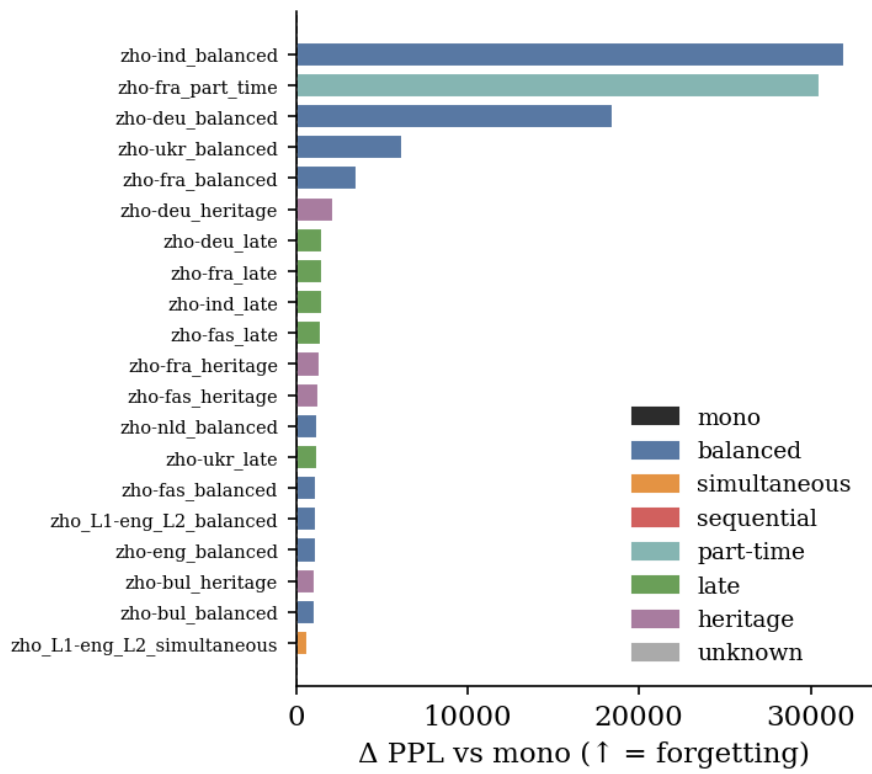
\includegraphics[width=\linewidth]{fig/zho_catastrophic_forgetting.png}
    \caption{Chinese Bilingual Models FLORES PPL compared to Chinese Monolingual FLORES PPL across different bilingual training conditions. \catherine{I'd like to discuss what we think we learn from this kind of analysis/figure. Not sure I totally get it!}}
    \label{fig:zho-ppl-catastrophic}
\end{figure}

\begin{figure}[!ht]
    \centering
    \includegraphics[width=\linewidth]{fig/03_barplot_by_type_zhoblimp.png}
    \caption{Average ZhoBLiMP performance on Bilingual Chinese \textsc{BabyBabelLM} models across different exposure schedules \texttt{balanced (bal), simultaneous, part-time, late, heritage} compared to monolingual BabybabelLM performance. The figure reports averages across non-Chinese L2.}
    \label{fig:zho-curricula-average}
\end{figure}



\paragraph{Effect of Data Quantity and Ordering} \autoref{fig:trilingual} show that the proportion of the training data (which is even in \texttt{balanced} compared to \texttt{heritage}) leads to more uniform monolingual BLiMP accuracies. 

\begin{figure}[!ht]
    \centering
    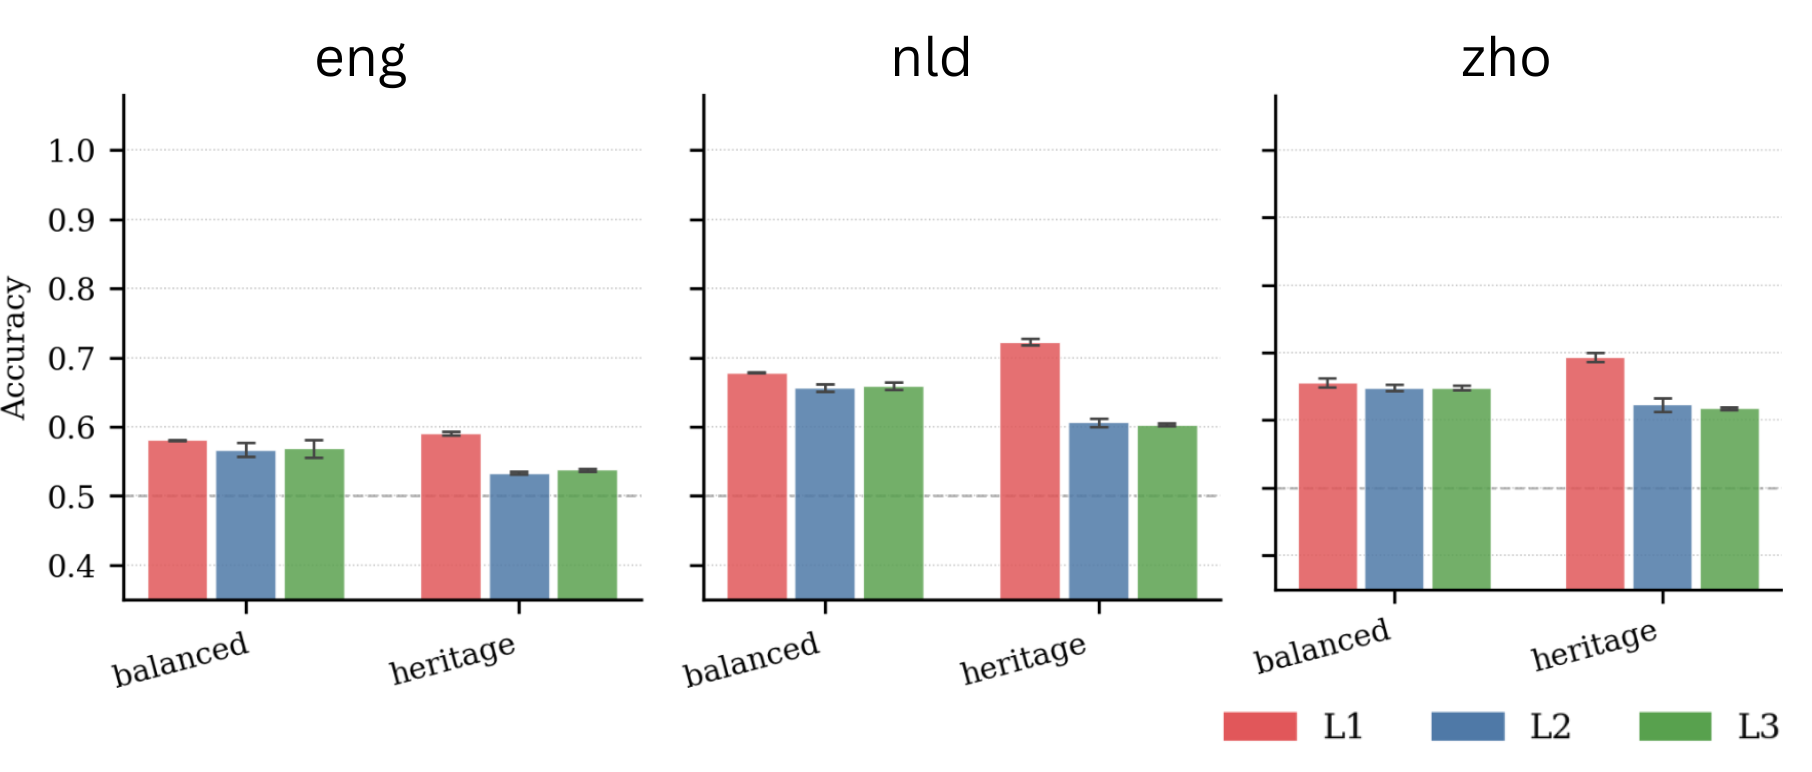
\includegraphics[width=\linewidth]{fig/trilingual-accuracy.png}
    \caption{\textbf{Effect of Data Ordering:} Accuracy of Trilingual \raisebox{-0.3em}{\includegraphics[height=1.2em]{fig/BeetleLM.png}} models on mono-BLiMP (\texttt{eng}:BLiMP; \texttt{nld}:BLiMP-NL and \texttt{zho}:Zho-BLiMP) accuracy across \texttt{balanced} and \texttt{heritage} exposure schedules. \catherine{This is super cool}}
    \label{fig:trilingual}
\end{figure}




\paragraph{Effect of EWC and MAML} \autoref{fig:ewc-maml} shows the effect of EWC and first-order MAML control parameters on BLiMP-NL and ZhoBLiMP accuracy across a trilingual sweep that jointly varies EWC strength $\lambda \in \{5,20,50,150\}$ and MAML adaptation horizon $h \in \{25,50,75,100\}$. Results show strong EWC $\lambda$ cause a reduction in ZhoBLiMP and BLiMP-NL accuracy, while higher MAML inner-loop adaptation horizons ($h = \{75, 100\})$ lead to marginally higher accuracy. The control parameter setting with EWC $\lambda=150$ + MAML $h=100$ achieves the highest accuracy on both Chinese and Dutch benchmarks.

\begin{figure}[!ht]
    \centering
    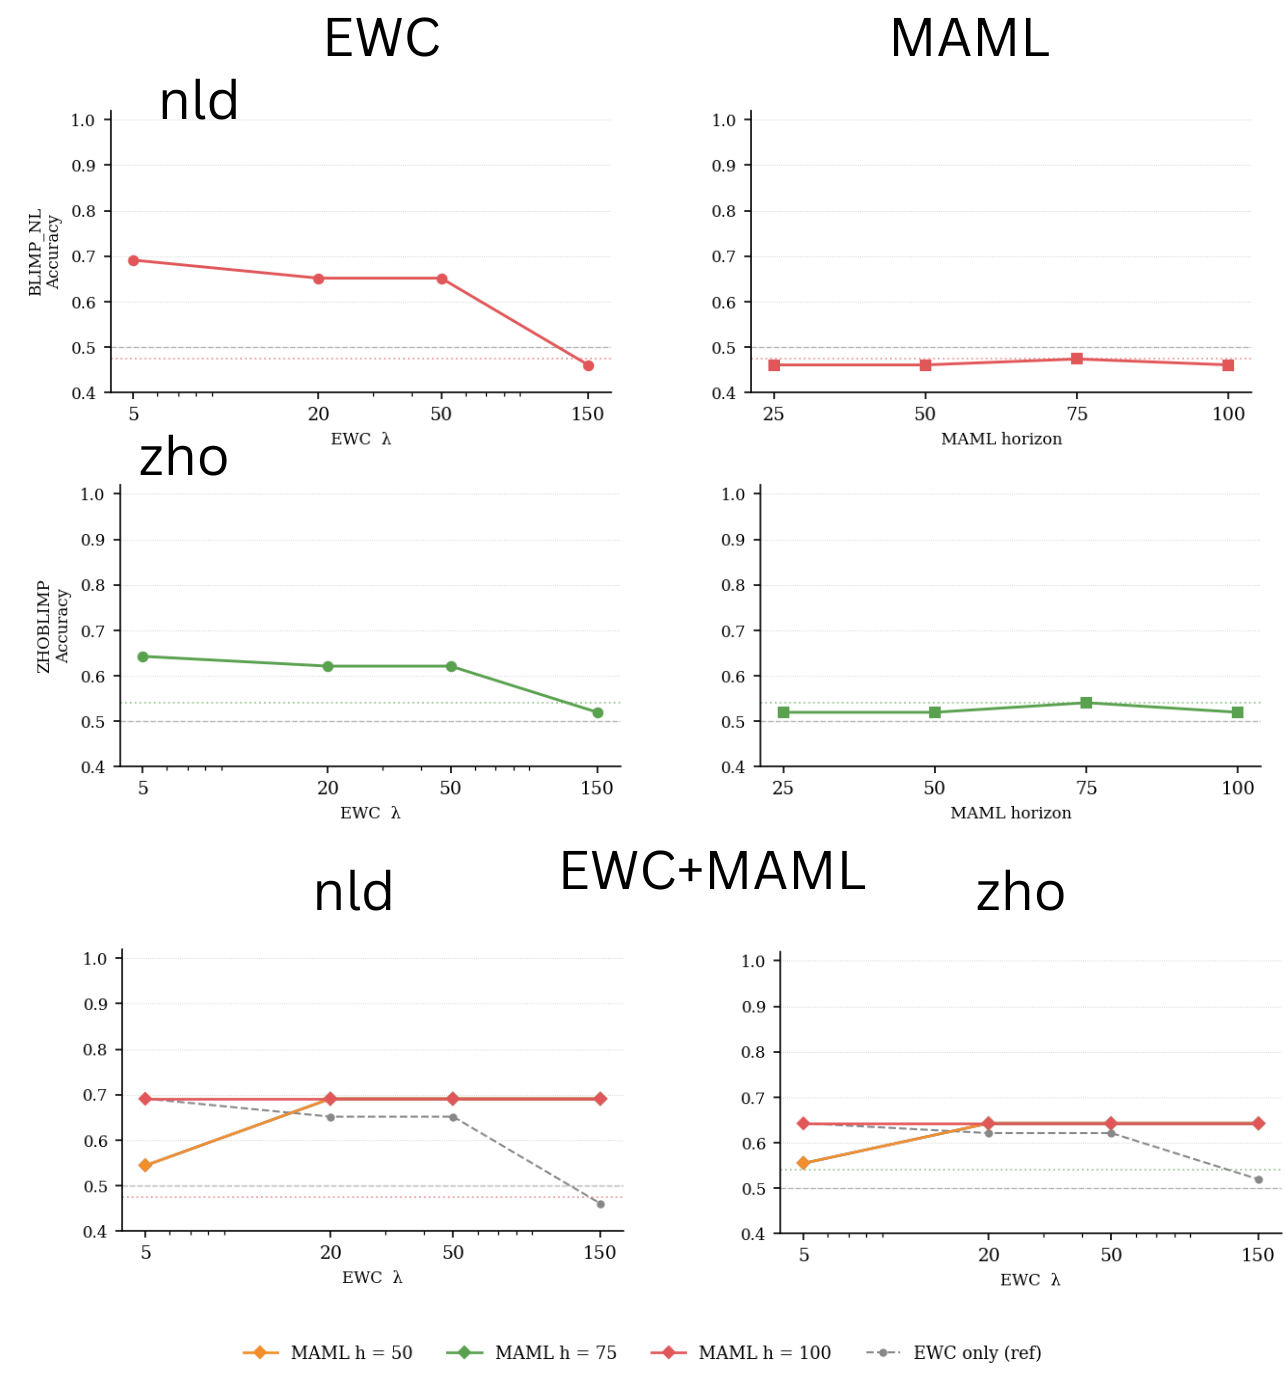
\includegraphics[width=\linewidth]{fig/ewc-maml.png}
    \caption{Effect of EWC and MAML on trilingual sequential regime \texttt{eng-nld-zho}. \catherine{We should be able to compare the beetles with comparable EWC, MAML, and EC+MAML conditions in one plot per language pair. This probably makes more sense for the psychometric fit analysis}}
    \label{fig:ewc-maml}
\end{figure}


\subsection{Catastrophic Forgetting}


% Table 5: Catastrophic forgetting by bilingual schedule
% Requires \usepackage{booktabs} in preamble
\begin{table}[t]
  \centering
  \small
  \caption{Catastrophic forgetting aggregated by acquisition schedule and language,
           sorted by \% sentences worse ascending.
           Mean $\Delta$-PPL: mean increase in per-sentence perplexity over the
           monolingual baseline;
           CF Log-Ratio: mean log perplexity ratio (positive = worse).
           Bold marks least forgetting per column.}
  \label{tab:forgetting}
  \begin{tabular}{llrrrl}
    \toprule
    Language & Schedule & Mean $\Delta$-PPL & CF Log-Ratio & \% Worse & $N$ \\
    \midrule
    German & Balanced & \textbf{157} & \textbf{+0.14} & \textbf{57} & 2 \\
    German & Sequential & 286 & +0.34 & 59 & 2 \\
    German & Part-time & 396 & +0.48 & 66 & 3 \\
    German & Heritage & 2418 & +0.76 & 67 & 6 \\
    German & Simultaneous & 1111 & +0.61 & 68 & 4 \\
    German & Late L2 & 118823 & +3.14 & 93 & 4 \\
    \midrule
    Chinese & Simultaneous & 676 & +2.90 & 100 & 1 \\
    \midrule
    Dutch & Heritage & 371 & +2.48 & 100 & 2 \\
    Dutch & Simultaneous & 774 & +3.17 & 100 & 3 \\
    Dutch & Balanced & 1048 & +3.24 & 100 & 8 \\
    \midrule
    Chinese & Late L2 & 1445 & +3.63 & 100 & 5 \\
    Chinese & Heritage & 1498 & +3.63 & 100 & 4 \\
    Chinese & Balanced & 7350 & +4.42 & 100 & 9 \\
    \midrule
    Dutch & Late L2 & 35979 & +4.86 & 100 & 2 \\
    Dutch & Part-time & 36071 & +5.14 & 100 & 2 \\
    \midrule
    Chinese & Part-time & 30567 & +6.65 & 100 & 1 \\
    \midrule
    Dutch & Sequential & 71758 & +7.66 & 100 & 1 \\
    \bottomrule
  \end{tabular}
\end{table}


\subsection{Bilingual Exposure Curricula}


\begin{figure*}[!ht]
    \centering
    \includegraphics[width=\linewidth]{fig/02_benchmark_by_language.png}
    \caption{Summary of Downstream peformance on Human-Scale Beetle Bilingual Models}
    \label{fig:placeholder}
\end{figure*}

\newpage 

\begin{figure}[!ht]
    \centering
    \includegraphics[width=0.8\linewidth]{fig/03_barplot_by_type_blimp_nl.png}
    %\caption{Caption}
    \label{fig:placeholder}
\end{figure}




\begin{figure}[!ht]
    \centering
    \includegraphics[width=0.8\linewidth]{fig/03_barplot_by_type_multiblimp.png}
    \caption{Comparison of Benchmark Performance by L1 and Exposure Schedule}
    \label{fig:placeholder}
\end{figure}


\newpage 


\subsection{Bilingual Learning Dynamics}


\begin{figure}[!ht]
    \centering
    \includegraphics[width=0.8\linewidth]{fig/01_learning_curves_blimp_nl.png}
    \caption{BLiMP-NL learning dynamics by checkpoint for bilingual language models by L1, categorised by exposure schedule}
    \label{fig:placeholder}
\end{figure}



\begin{figure}[!ht]
    \centering
    \includegraphics[width=0.8\linewidth]{fig/01_learning_curves_zhoblimp.png}
    \caption{ZhoBLiMP learning dynamics by checkpoint for bilingual language models by L1, categorised by exposure schedule}
    \label{fig:placeholder}
\end{figure}


\newpage 
\begin{figure}[!ht]
    \centering
    \includegraphics[width=\linewidth]{fig/01_learning_curves_multiblimp.png}
    \caption{MultiBLiMP learning dynamics by checkpoint for bilingual language models by L1, categorised by exposure schedule}
    \label{fig:placeholder}
  \end{figure}




\newpage 

\subsection{Trilingual Learning Dynamics}


\begin{figure}[!ht]
    \centering
    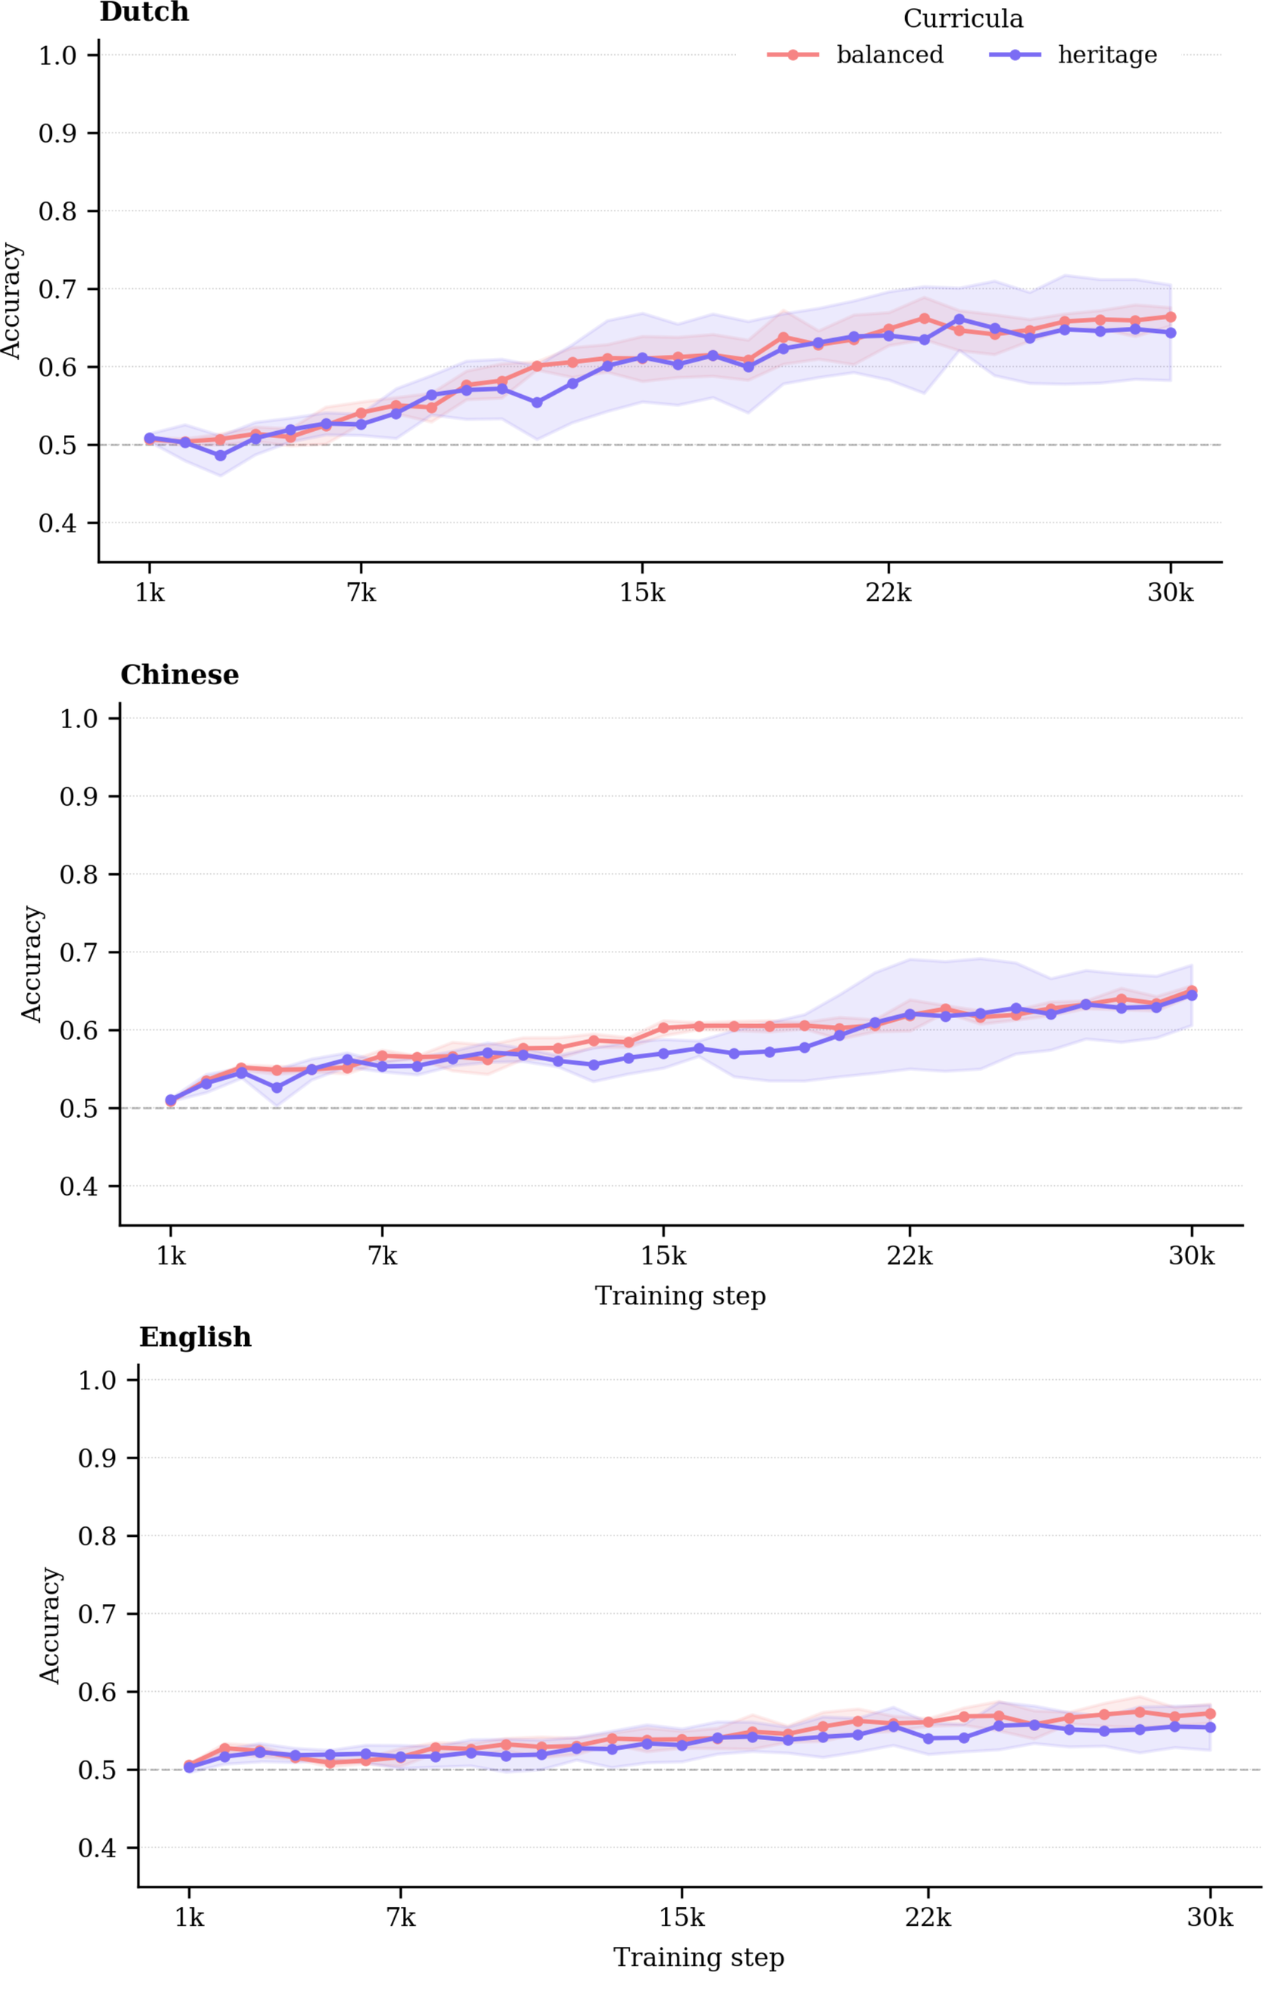
\includegraphics[width=0.8\linewidth]{fig/trilingual-learning-dynamics.png}
    \caption{Trilingual Language-Specific BLiMP learning dynamics}
    \label{fig:placeholder}
\end{figure}


\newpage 

\section{Bilingual Perplexity Results} \label{apdx-PPL}


\begin{figure}[!ht]
    \centering
    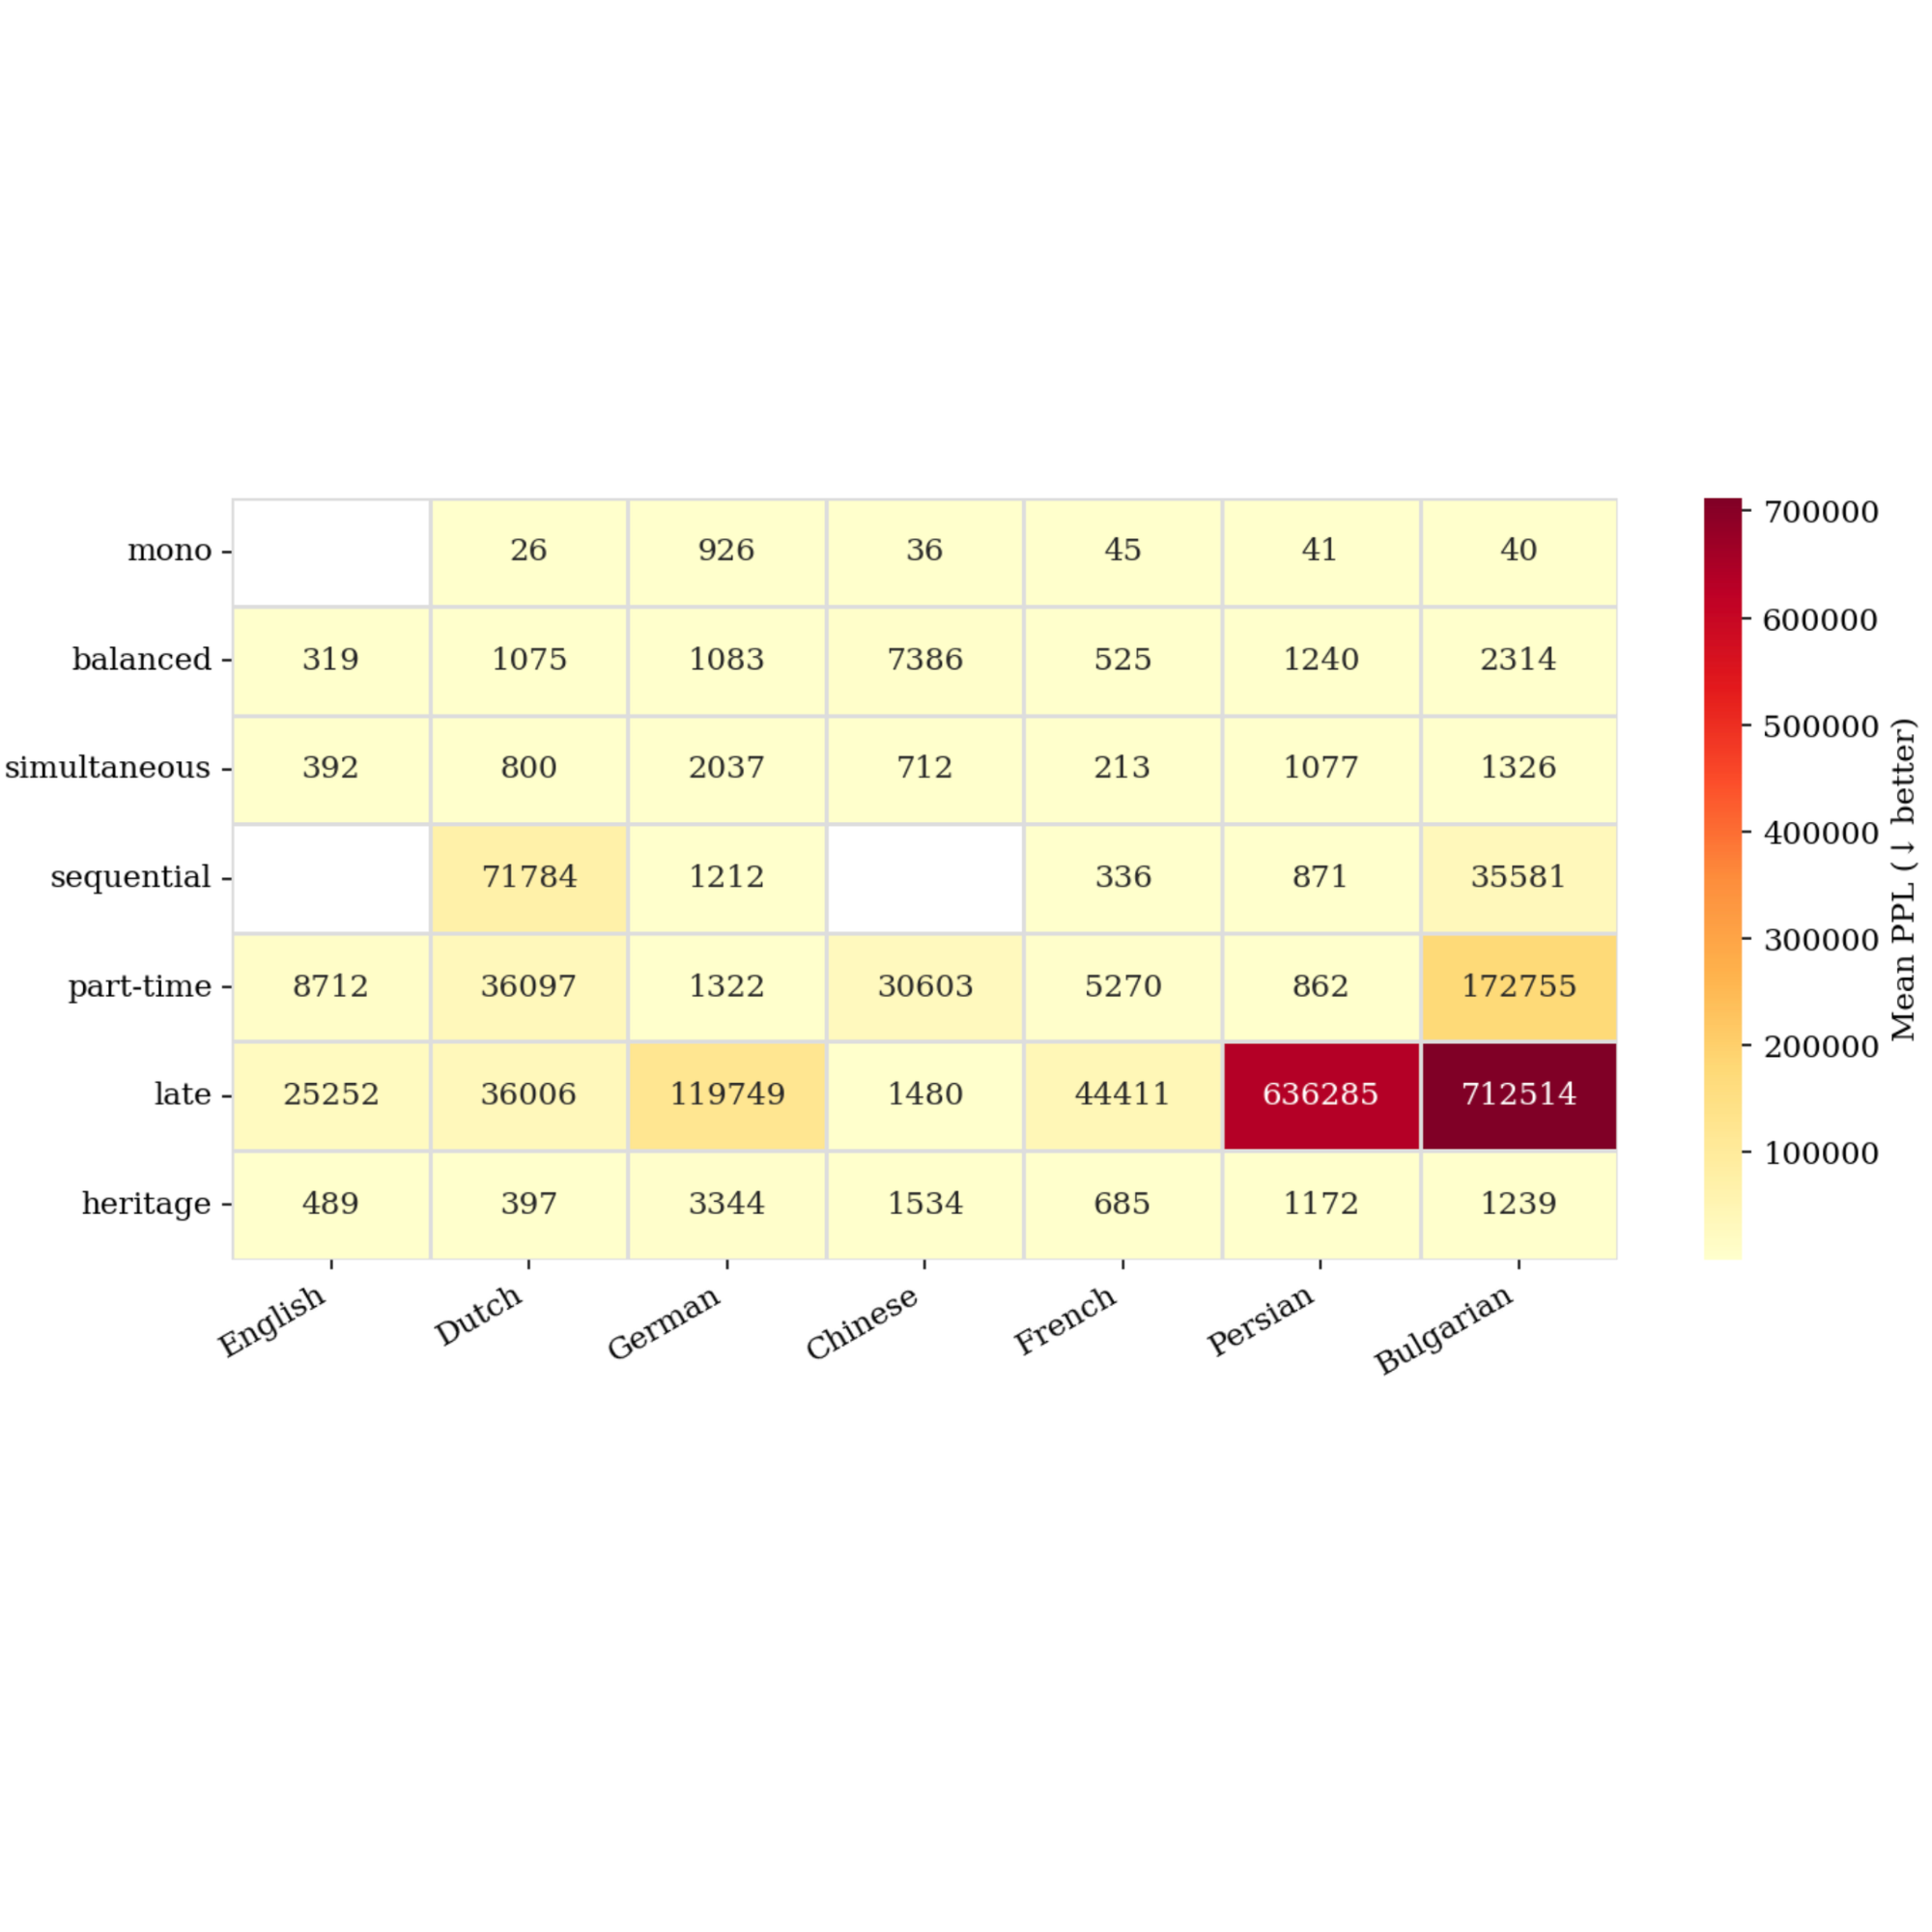
\includegraphics[width=\linewidth]{fig/mean_ppl.png}
    \caption{Final FLORES PPL for bilingual models by L1 and exposure schedule}
    \label{fig:placeholder}
\end{figure}



\newpage 


\begin{figure}[!ht]
    \centering
    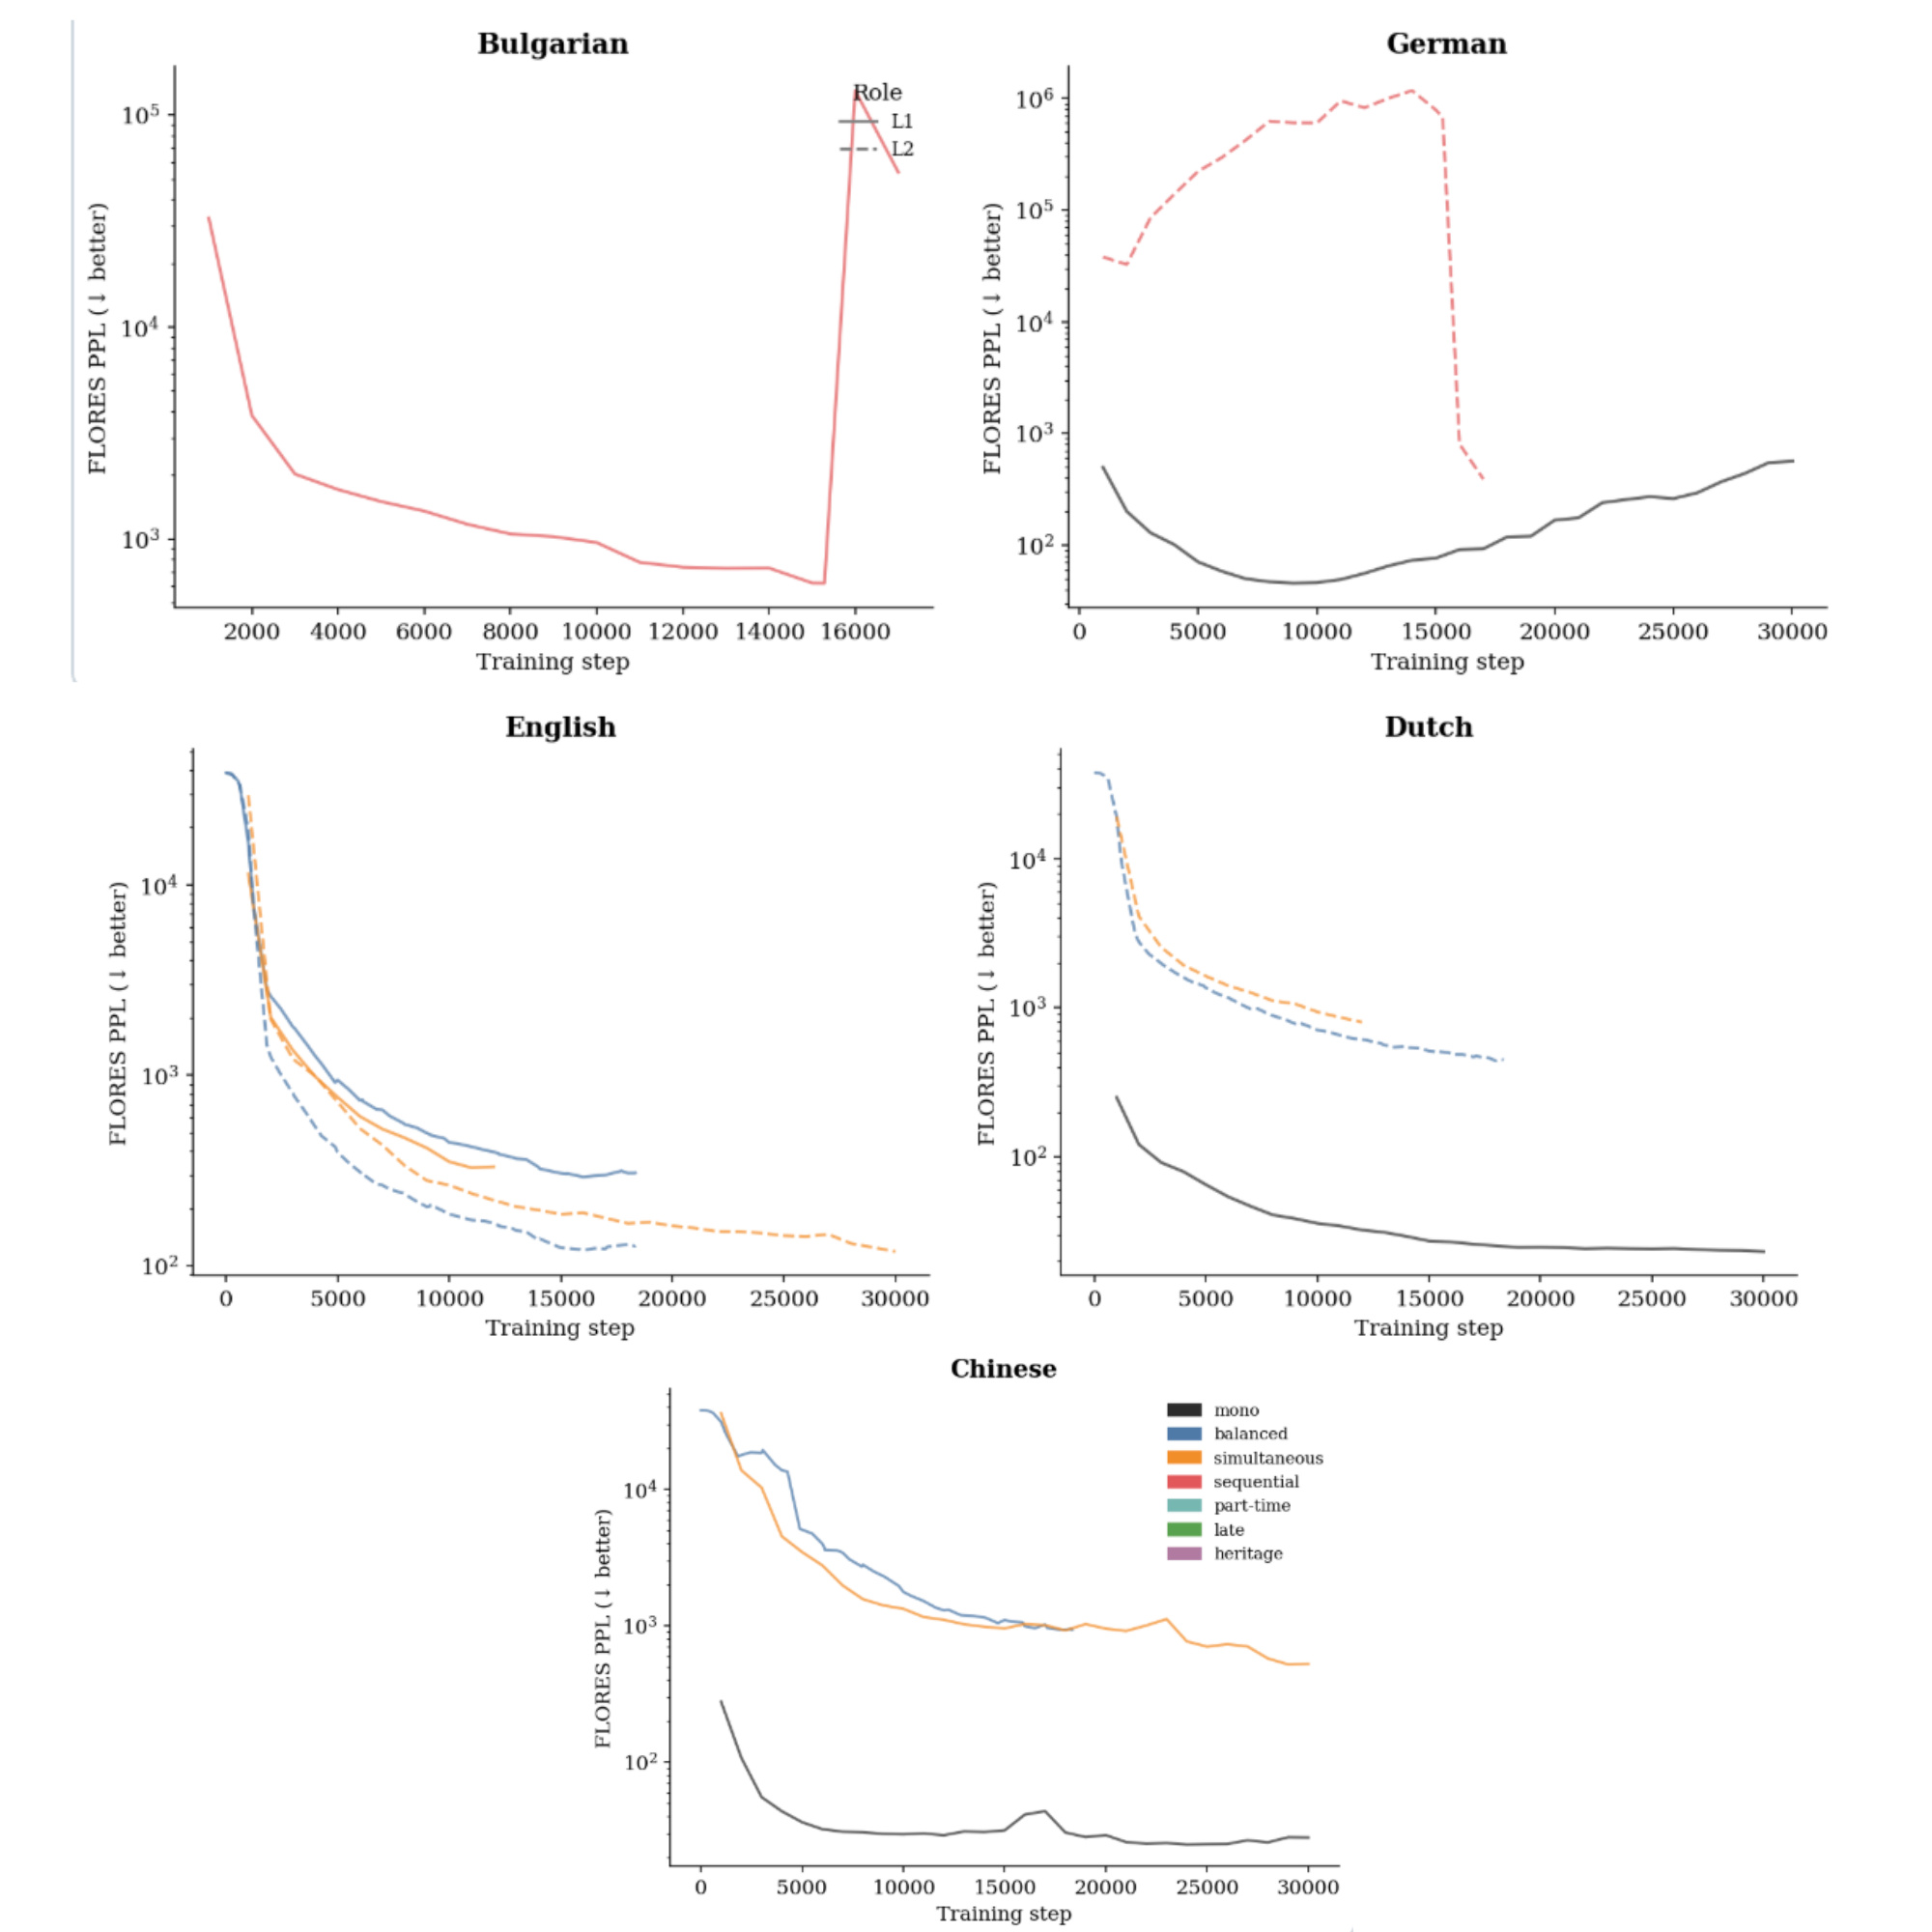
\includegraphics[width=\linewidth]{fig/PPL_learning_curves.png}
    \caption{Language-Specific FLORES PPL across bilingual training runs by exposure curricula}
    \label{fig:placeholder}
\end{figure}


\newpage 

\section{Additional Learning Conditions}

\subsection{Bilingual}
\begin{itemize}
    \item \textbf{B4 – Immersion Bilingual:} Initially monolingual L1, followed by a rapid but \textbf{smoothed} transition to L2-dominant exposure, with sparse L1 episodes.
    \begin{itemize}
        \item \textit{Mechanisms:} weak EWC, LR spike at immersion, no MAML
        \item \textit{Cognitive properties:} rapid restructuring under pressure, partial retention
    \end{itemize}

    \item \textbf{B5 – Code-Switching / Mixed Context:} Globally balanced exposure, but with short episodes, high switching frequency, and domain-conditioned usage (e.g., L1=home, L2=peers).
    \begin{itemize}
        \item \textit{Mechanisms:} strong MAML, no EWC, slight LR noise
        \item \textit{Cognitive properties:} context-sensitive switching, clustered input
    \end{itemize}
\end{itemize} 

\subsection{L2}



\section{Rough – Figure Ideas}

\suchir{Tatsuya's L2LM paper and thesis – PPL, BLiMP typology, reading time + per-sentence examples.}

\suchir{BLiSS v BLiMP}

\suchir{MECO v CELER? – but don't think CELER is available}


